%*************************************************************************
% A Classic Thesis Style
% An Homage to The Elements of Typographic Style
%
% Copyright (C) 2017 André Miede and Ivo Pletikosić
%
% If you like the style then I would appreciate a postcard. My address
% can be found in the file ClassicThesis.pdf. A collection of the
% postcards I received so far is available online at
% http://postcards.miede.de
%
% License:
% This program is free software; you can redistribute it and/or modify
% it under the terms of the GNU General Public License as published by
% the Free Software Foundation; either version 2 of the License, or
% (at your option) any later version.
%
% This program is distributed in the hope that it will be useful,
% but WITHOUT ANY WARRANTY; without even the implied warranty of
% MERCHANTABILITY or FITNESS FOR A PARTICULAR PURPOSE.  See the
% GNU General Public License for more details.
%
% You should have received a copy of the GNU General Public License
% along with this program; see the file COPYING.  If not, write to
% the Free Software Foundation, Inc., 59 Temple Place - Suite 330,
% Boston, MA 02111-1307, USA.
%
% PLEASE SEE ALSO THE AUTHORS' NOTE REGARDING THIS LICENSE
% IN THE DOCUMENTATION (ClassicThesis.pdf --> Chapter 1 / Chapter01.tex)
%*************************************************************************
\RequirePackage{silence} % :-\
    \WarningFilter{scrreprt}{Usage of package `titlesec'}
    %\WarningFilter{scrreprt}{Activating an ugly workaround}
    \WarningFilter{titlesec}{Non standard sectioning command detected}
\documentclass[ titlepage,numbers=noenddot,headinclude,twoside, openright, %1headlines,% letterpaper a4paper
                footinclude=true,cleardoublepage=empty,abstractoff, % <--- obsolete, remove (todo)
                BCOR=5mm,paper=a4,fontsize=11pt,%11pt,a4paper,%
                ngerman,american,% openright
                ]{scrreprt}

%*************************************************************************
% Note: Make all your adjustments in here
%*************************************************************************
% ****************************************************************************************************
% hdathesis-config.tex 
% Use it at the beginning of your thesis.tex, or as a LaTeX Preamble 
% in your thesis.{tex,lyx} with % ****************************************************************************************************
% hdathesis-config.tex 
% Use it at the beginning of your thesis.tex, or as a LaTeX Preamble 
% in your thesis.{tex,lyx} with % ****************************************************************************************************
% hdathesis-config.tex 
% Use it at the beginning of your thesis.tex, or as a LaTeX Preamble 
% in your thesis.{tex,lyx} with \input{hdathesis-config}
% ****************************************************************************************************

% ****************************************************************************************************
% 1. Personal data and user ad-hoc commands
% ****************************************************************************************************
\newcommand{\myTitle}{Vergleich von Isolationsframeworks für den Containerbetrieb\xspace}
%\newcommand{\mySubtitle}{An Homage to The Elements of Typographic Style\xspace}
\newcommand{\myDegree}{Bachelor of Science (B.Sc.)\xspace} 
%\newcommand{\myDegree}{Bachelor of Arts (B.A.)\xspace}
%\newcommand{\myDegree}{Master of Science (M.Sc.)\xspace}
%\newcommand{\myDegree}{Master of Arts (M.A.)\xspace}
\newcommand{\myName}{Tim Stoffel\xspace}
\newcommand{\myId}{750116\xspace}
\newcommand{\myProf}{Prof. Dr.-Ing. Michael von Rüden\xspace}
\newcommand{\myOtherProf}{Dominik Sauer\xspace}
\newcommand{\myFaculty}{Fachbereich Informatik\xspace}
\newcommand{\myUni}{Hochschule Darmstadt\xspace}
\newcommand{\myLocation}{Darmstadt\xspace}
\newcommand{\myTime}{06. März 2020\xspace}
\newcommand{\myVersion}{version 1.0\xspace}

% ****************************************************************************************************
% 2. Is it a master thesis?
% ****************************************************************************************************
%\PassOptionsToPackage{master}{hdahesis} % uncomment if this is a master thesis 

% ****************************************************************************************************
% 3. Does the thesis have a lock flag?
% ****************************************************************************************************
%\PassOptionsToPackage{lockflag}{hdathesis} % uncomment if this thesis has a lock flag 

% ****************************************************************************************************
% 4. Loading some handy packages
% ****************************************************************************************************
% ****************************************************************************************************
% Packages with options that might require adjustments
% ****************************************************************************************************

%\PassOptionsToPackage{ngerman,american}{babel}   % change this to your language(s)
% Spanish languages need extra options in order to work with this template
%\PassOptionsToPackage{spanish,es-lcroman}{babel}
\usepackage{babel}


% ****************************************************************************************************

% ****************************************************************************************************
% 1. Personal data and user ad-hoc commands
% ****************************************************************************************************
\newcommand{\myTitle}{Vergleich von Isolationsframeworks für den Containerbetrieb\xspace}
%\newcommand{\mySubtitle}{An Homage to The Elements of Typographic Style\xspace}
\newcommand{\myDegree}{Bachelor of Science (B.Sc.)\xspace} 
%\newcommand{\myDegree}{Bachelor of Arts (B.A.)\xspace}
%\newcommand{\myDegree}{Master of Science (M.Sc.)\xspace}
%\newcommand{\myDegree}{Master of Arts (M.A.)\xspace}
\newcommand{\myName}{Tim Stoffel\xspace}
\newcommand{\myId}{750116\xspace}
\newcommand{\myProf}{Prof. Dr.-Ing. Michael von Rüden\xspace}
\newcommand{\myOtherProf}{Dominik Sauer\xspace}
\newcommand{\myFaculty}{Fachbereich Informatik\xspace}
\newcommand{\myUni}{Hochschule Darmstadt\xspace}
\newcommand{\myLocation}{Darmstadt\xspace}
\newcommand{\myTime}{06. März 2020\xspace}
\newcommand{\myVersion}{version 1.0\xspace}

% ****************************************************************************************************
% 2. Is it a master thesis?
% ****************************************************************************************************
%\PassOptionsToPackage{master}{hdahesis} % uncomment if this is a master thesis 

% ****************************************************************************************************
% 3. Does the thesis have a lock flag?
% ****************************************************************************************************
%\PassOptionsToPackage{lockflag}{hdathesis} % uncomment if this thesis has a lock flag 

% ****************************************************************************************************
% 4. Loading some handy packages
% ****************************************************************************************************
% ****************************************************************************************************
% Packages with options that might require adjustments
% ****************************************************************************************************

%\PassOptionsToPackage{ngerman,american}{babel}   % change this to your language(s)
% Spanish languages need extra options in order to work with this template
%\PassOptionsToPackage{spanish,es-lcroman}{babel}
\usepackage{babel}


% ****************************************************************************************************

% ****************************************************************************************************
% 1. Personal data and user ad-hoc commands
% ****************************************************************************************************
\newcommand{\myTitle}{Vergleich von Isolationsframeworks für den Containerbetrieb\xspace}
%\newcommand{\mySubtitle}{An Homage to The Elements of Typographic Style\xspace}
\newcommand{\myDegree}{Bachelor of Science (B.Sc.)\xspace} 
%\newcommand{\myDegree}{Bachelor of Arts (B.A.)\xspace}
%\newcommand{\myDegree}{Master of Science (M.Sc.)\xspace}
%\newcommand{\myDegree}{Master of Arts (M.A.)\xspace}
\newcommand{\myName}{Tim Stoffel\xspace}
\newcommand{\myId}{750116\xspace}
\newcommand{\myProf}{Prof. Dr.-Ing. Michael von Rüden\xspace}
\newcommand{\myOtherProf}{Dominik Sauer\xspace}
\newcommand{\myFaculty}{Fachbereich Informatik\xspace}
\newcommand{\myUni}{Hochschule Darmstadt\xspace}
\newcommand{\myLocation}{Darmstadt\xspace}
\newcommand{\myTime}{06. März 2020\xspace}
\newcommand{\myVersion}{version 1.0\xspace}

% ****************************************************************************************************
% 2. Is it a master thesis?
% ****************************************************************************************************
%\PassOptionsToPackage{master}{hdahesis} % uncomment if this is a master thesis 

% ****************************************************************************************************
% 3. Does the thesis have a lock flag?
% ****************************************************************************************************
%\PassOptionsToPackage{lockflag}{hdathesis} % uncomment if this thesis has a lock flag 

% ****************************************************************************************************
% 4. Loading some handy packages
% ****************************************************************************************************
% ****************************************************************************************************
% Packages with options that might require adjustments
% ****************************************************************************************************

%\PassOptionsToPackage{ngerman,american}{babel}   % change this to your language(s)
% Spanish languages need extra options in order to work with this template
%\PassOptionsToPackage{spanish,es-lcroman}{babel}
\usepackage{babel}


% ****************************************************************************************************
% classicthesis-config.tex
% formerly known as loadpackages.sty, classicthesis-ldpkg.sty, and classicthesis-preamble.sty
% Use it at the beginning of your ClassicThesis.tex, or as a LaTeX Preamble
% in your ClassicThesis.{tex,lyx} with % ****************************************************************************************************
% classicthesis-config.tex
% formerly known as loadpackages.sty, classicthesis-ldpkg.sty, and classicthesis-preamble.sty
% Use it at the beginning of your ClassicThesis.tex, or as a LaTeX Preamble
% in your ClassicThesis.{tex,lyx} with % ****************************************************************************************************
% classicthesis-config.tex
% formerly known as loadpackages.sty, classicthesis-ldpkg.sty, and classicthesis-preamble.sty
% Use it at the beginning of your ClassicThesis.tex, or as a LaTeX Preamble
% in your ClassicThesis.{tex,lyx} with \input{classicthesis-config}
% ****************************************************************************************************
% If you like the classicthesis, then I would appreciate a postcard.
% My address can be found in the file ClassicThesis.pdf. A collection
% of the postcards I received so far is available online at
% http://postcards.miede.de
% ****************************************************************************************************


% ****************************************************************************************************
% 0. Set the encoding of your files. UTF-8 is the only sensible encoding nowadays. If you can't read
% äöüßáéçèê∂åëæƒÏ€ then change the encoding setting in your editor, not the line below. If your editor
% does not support utf8 use another editor!
% ****************************************************************************************************
\PassOptionsToPackage{utf8}{inputenc}
  \usepackage{inputenc}

% ****************************************************************************************************
% 1. Configure classicthesis for your needs here, e.g., remove "drafting" below
% in order to deactivate the time-stamp on the pages
% (see ClassicThesis.pdf for more information):
% ****************************************************************************************************
\PassOptionsToPackage{
  drafting=false,   % print version information on the bottom of the pages
  tocaligned=false, % the left column of the toc will be aligned (no indentation)
  dottedtoc=true,   % page numbers in ToC flushed right
  parts=true,       % use part division
  eulerchapternumbers=true, % use AMS Euler for chapter font (otherwise Palatino)
  linedheaders=false,       % chaper headers will have line above and beneath
  floatperchapter=true,     % numbering per chapter for all floats (i.e., Figure 1.1)
  listings=true,    % load listings package and setup LoL
  subfig=true,      % setup for preloaded subfig package
  eulermath=true,  % use awesome Euler fonts for mathematical formulae (only with pdfLaTeX)
  beramono=true,    % toggle a nice monospaced font (w/ bold)
  minionpro=false   % setup for minion pro font; use minion pro small caps as well (only with pdfLaTeX)
}{classicthesis}


% ****************************************************************************************************
% 2. Personal data and user ad-hoc commands
% ****************************************************************************************************
%\newcommand{\myTitle}{A Classic Thesis Style\xspace}
%\newcommand{\mySubtitle}{An Homage to The Elements of Typographic Style\xspace}
%\newcommand{\myDegree}{Doktor-Ingenieur (Dr.-Ing.)\xspace}
%\newcommand{\myName}{André Miede\xspace}
%\newcommand{\myProf}{Put name here\xspace}
%\newcommand{\myOtherProf}{Put name here\xspace}
%\newcommand{\mySupervisor}{Put name here\xspace}
%\newcommand{\myFaculty}{Put data here\xspace}
%\newcommand{\myDepartment}{Put data here\xspace}
%\newcommand{\myUni}{Put data here\xspace}
%\newcommand{\myLocation}{Saarbrücken\xspace}
%\newcommand{\myTime}{October 2017\xspace}
%\newcommand{\myVersion}{version 4.4}

% ********************************************************************
% Setup, finetuning, and useful commands
% ********************************************************************
\newcounter{dummy} % necessary for correct hyperlinks (to index, bib, etc.)
\newlength{\abcd} % for ab..z string length calculation
\providecommand{\mLyX}{L\kern-.1667em\lower.25em\hbox{Y}\kern-.125emX\@}
\newcommand{\ie}{i.\,e.}
\newcommand{\Ie}{I.\,e.}
\newcommand{\eg}{e.\,g.}
\newcommand{\Eg}{E.\,g.}
% ****************************************************************************************************


% ****************************************************************************************************
% 3. Loading some handy packages
% ****************************************************************************************************
% ********************************************************************
% Packages with options that might require adjustments
% ********************************************************************
\PassOptionsToPackage{american, ngerman}{babel}   % change this to your language(s), main language last
% Spanish languages need extra options in order to work with this template
%\PassOptionsToPackage{spanish,es-lcroman}{babel}
\usepackage{babel}

\usepackage{csquotes}

\PassOptionsToPackage{%
  %backend=biber,bibencoding=utf8, %instead of bibtex
  backend=bibtex8,bibencoding=ascii,%
  language=auto,%
  style=numeric-comp,%
  %style=alphabetic,%
  %style=authoryear-comp, % Author 1999, 2010
  %bibstyle=authoryear,dashed=false, % dashed: substitute rep. author with ---
  sorting=nyt, % name, year, title
  maxbibnames=10, % default: 3, et al.
  backref=false,%
  natbib=true % natbib compatibility mode (\citep and \citet still work)
}{biblatex}
  \usepackage{biblatex}

\PassOptionsToPackage{fleqn}{amsmath}       % math environments and more by the AMS
  \usepackage{amsmath}

\PassOptionsToPackage{doublespacing}{hdathesis}  % options: abbrev exam big wiwi english master
  \usepackage{hdathesis}

% ********************************************************************
% General useful packages
% ********************************************************************
\PassOptionsToPackage{T1}{fontenc} % T2A for cyrillics
  \usepackage{fontenc}
\usepackage{textcomp} % fix warning with missing font shapes
\usepackage{scrhack} % fix warnings when using KOMA with listings package
\usepackage{xspace} % to get the spacing after macros right
\usepackage{mparhack} % get marginpar right
%\usepackage{fixltx2e} % fixes some LaTeX stuff --> since 2015 in the LaTeX kernel (see below)
% \usepackage[latest]{latexrelease} % emulate newer kernel version if older is detected
\PassOptionsToPackage{printonlyused,smaller}{acronym}
  \usepackage{acronym} % nice macros for handling all acronyms in the thesis
  %\renewcommand{\bflabel}[1]{{#1}\hfill} % fix the list of acronyms --> no longer working
  %\renewcommand*{\acsfont}[1]{\textsc{#1}}
  %\renewcommand*{\aclabelfont}[1]{\acsfont{#1}}
  %\def\bflabel#1{{#1\hfill}}
  \def\bflabel#1{{\acsfont{#1}\hfill}}
  \def\aclabelfont#1{\acsfont{#1}}
% ****************************************************************************************************
%\usepackage{pgfplots} % External TikZ/PGF support (thanks to Andreas Nautsch)
%\usetikzlibrary{external}
%\tikzexternalize[mode=list and make, prefix=ext-tikz/]
% ****************************************************************************************************


% ****************************************************************************************************
% 4. Setup floats: tables, (sub)figures, and captions
% ****************************************************************************************************
\usepackage{tabularx} % better tables
  \setlength{\extrarowheight}{3pt} % increase table row height
\newcommand{\tableheadline}[1]{\multicolumn{1}{c}{\spacedlowsmallcaps{#1}}}
\newcommand{\myfloatalign}{\centering} % to be used with each float for alignment
\usepackage{caption}
% Thanks to cgnieder and Claus Lahiri
% http://tex.stackexchange.com/questions/69349/spacedlowsmallcaps-in-caption-label
% [REMOVED DUE TO OTHER PROBLEMS, SEE ISSUE #82]
%\DeclareCaptionLabelFormat{smallcaps}{\bothIfFirst{#1}{~}\MakeTextLowercase{\textsc{#2}}}
%\captionsetup{font=small,labelformat=smallcaps} % format=hang,
\captionsetup{font=small} % format=hang,
\usepackage{subfig}
% ****************************************************************************************************


% ****************************************************************************************************
% 5. Setup code listings
% ****************************************************************************************************
\usepackage{listings}
%\lstset{emph={trueIndex,root},emphstyle=\color{BlueViolet}}%\underbar} % for special keywords
\lstset{language=[LaTeX]Tex,%C++,
  morekeywords={PassOptionsToPackage,selectlanguage},
  keywordstyle=\color{RoyalBlue},%\bfseries,
  basicstyle=\small\ttfamily,
  %identifierstyle=\color{NavyBlue},
  commentstyle=\color{Green}\ttfamily,
  stringstyle=\rmfamily,
  numbers=none,%left,%
  numberstyle=\scriptsize,%\tiny
  stepnumber=5,
  numbersep=8pt,
  showstringspaces=false,
  breaklines=true,
  %frameround=ftff,
  %frame=single,
  belowcaptionskip=.75\baselineskip
  %frame=L
}
% ****************************************************************************************************


% ****************************************************************************************************
% 6. PDFLaTeX, hyperreferences, and citation backreferences
% ****************************************************************************************************
% ********************************************************************
% Using PDFLaTeX
% ********************************************************************
\PassOptionsToPackage{hyperfootnotes=false,pdfpagelabels}{hyperref}
  \usepackage{hyperref}  % backref linktocpage pagebackref
%\ifpdf
%\pdfcompresslevel=9
%\pdfadjustspacing=1
%\fi
%\PassOptionsToPackage{pdftex}{graphicx} %%%IVO: driver will be chosen automatically
  \usepackage{graphicx}


% ********************************************************************
% Hyperreferences
% ********************************************************************
\hypersetup{%
  %draft, % hyperref's draft mode, for printing see below
  colorlinks=true, linktocpage=true, pdfstartpage=3, pdfstartview=FitV,%
  % uncomment the following line if you want to have black links (e.g., for printing)
  %colorlinks=false, linktocpage=false, pdfstartpage=3, pdfstartview=FitV, pdfborder={0 0 0},%
  breaklinks=true, pdfpagemode=UseNone, pageanchor=true, pdfpagemode=UseOutlines,%
  plainpages=false, bookmarksnumbered, bookmarksopen=true, bookmarksopenlevel=1,%
  hypertexnames=true, pdfhighlight=/O,%nesting=true,%frenchlinks,%
  urlcolor=webbrown, linkcolor=RoyalBlue, citecolor=webgreen, %pagecolor=RoyalBlue,%
  %urlcolor=Black, linkcolor=Black, citecolor=Black, %pagecolor=Black,%
  pdftitle={\myTitle},%
  pdfauthor={\textcopyright\ \myName, \myUni, \myFaculty},%
  pdfsubject={},%
  pdfkeywords={},%
  pdfcreator={pdfLaTeX},%
  pdfproducer={LaTeX with hyperref and classicthesis}%
}

% ********************************************************************
% Setup autoreferences
% ********************************************************************
% There are some issues regarding autorefnames
% http://www.ureader.de/msg/136221647.aspx
% http://www.tex.ac.uk/cgi-bin/texfaq2html?label=latexwords
% you have to redefine the makros for the
% language you use, e.g., american, ngerman
% (as chosen when loading babel/AtBeginDocument)
% ********************************************************************
\makeatletter
\@ifpackageloaded{babel}%
  {%
    \addto\extrasamerican{%
      \renewcommand*{\figureautorefname}{Figure}%
      \renewcommand*{\tableautorefname}{Table}%
      \renewcommand*{\partautorefname}{Part}%
      \renewcommand*{\chapterautorefname}{Chapter}%
      \renewcommand*{\sectionautorefname}{Section}%
      \renewcommand*{\subsectionautorefname}{Section}%
      \renewcommand*{\subsubsectionautorefname}{Section}%
    }%
    \addto\extrasngerman{%
      \renewcommand*{\paragraphautorefname}{Absatz}%
      \renewcommand*{\subparagraphautorefname}{Unterabsatz}%
      \renewcommand*{\footnoteautorefname}{Fu\"snote}%
      \renewcommand*{\FancyVerbLineautorefname}{Zeile}%
      \renewcommand*{\theoremautorefname}{Theorem}%
      \renewcommand*{\appendixautorefname}{Anhang}%
      \renewcommand*{\equationautorefname}{Gleichung}%
      \renewcommand*{\itemautorefname}{Punkt}%
    }%
      % Fix to getting autorefs for subfigures right (thanks to Belinda Vogt for changing the definition)
      \providecommand{\subfigureautorefname}{\figureautorefname}%
    }{\relax}
\makeatother


% ****************************************************************************************************
% 7. Last calls before the bar closes
% ****************************************************************************************************
% ********************************************************************
% Development Stuff
% ********************************************************************
\listfiles
%\PassOptionsToPackage{l2tabu,orthodox,abort}{nag}
%  \usepackage{nag}
%\PassOptionsToPackage{warning, all}{onlyamsmath}
%  \usepackage{onlyamsmath}

% ********************************************************************
% Last, but not least...
% ********************************************************************
\usepackage{classicthesis}
% ****************************************************************************************************


% ****************************************************************************************************
% 8. Further adjustments (experimental)
% ****************************************************************************************************
% ********************************************************************
% Changing the text area
% ********************************************************************
%\areaset[current]{312pt}{761pt} % 686 (factor 2.2) + 33 head + 42 head \the\footskip
%\setlength{\marginparwidth}{7em}%
%\setlength{\marginparsep}{2em}%

% ********************************************************************
% Using different fonts
% ********************************************************************
%\usepackage[oldstylenums]{kpfonts} % oldstyle notextcomp
%\usepackage[osf]{libertine}
%\usepackage[light,condensed,math]{iwona}
%\renewcommand{\sfdefault}{iwona}
%\usepackage{lmodern} % <-- no osf support :-(
%\usepackage{cfr-lm} %
%\usepackage[urw-garamond]{mathdesign} <-- no osf support :-(
%\usepackage[default,osfigures]{opensans} % scale=0.95
%\usepackage[sfdefault]{FiraSans}
% ********************************************************************
% \usepackage[largesc,osf]{newpxtext}
% Used to fix these:
% https://bitbucket.org/amiede/classicthesis/issues/139/italics-in-pallatino-capitals-chapter
% https://bitbucket.org/amiede/classicthesis/issues/45/problema-testatine-su-classicthesis-style
% ********************************************************************
%\linespread{1.05} % a bit more for Palatino
% ****************************************************************************************************

% ****************************************************************************************************
% If you like the classicthesis, then I would appreciate a postcard.
% My address can be found in the file ClassicThesis.pdf. A collection
% of the postcards I received so far is available online at
% http://postcards.miede.de
% ****************************************************************************************************


% ****************************************************************************************************
% 0. Set the encoding of your files. UTF-8 is the only sensible encoding nowadays. If you can't read
% äöüßáéçèê∂åëæƒÏ€ then change the encoding setting in your editor, not the line below. If your editor
% does not support utf8 use another editor!
% ****************************************************************************************************
\PassOptionsToPackage{utf8}{inputenc}
  \usepackage{inputenc}

% ****************************************************************************************************
% 1. Configure classicthesis for your needs here, e.g., remove "drafting" below
% in order to deactivate the time-stamp on the pages
% (see ClassicThesis.pdf for more information):
% ****************************************************************************************************
\PassOptionsToPackage{
  drafting=false,   % print version information on the bottom of the pages
  tocaligned=false, % the left column of the toc will be aligned (no indentation)
  dottedtoc=true,   % page numbers in ToC flushed right
  parts=true,       % use part division
  eulerchapternumbers=true, % use AMS Euler for chapter font (otherwise Palatino)
  linedheaders=false,       % chaper headers will have line above and beneath
  floatperchapter=true,     % numbering per chapter for all floats (i.e., Figure 1.1)
  listings=true,    % load listings package and setup LoL
  subfig=true,      % setup for preloaded subfig package
  eulermath=true,  % use awesome Euler fonts for mathematical formulae (only with pdfLaTeX)
  beramono=true,    % toggle a nice monospaced font (w/ bold)
  minionpro=false   % setup for minion pro font; use minion pro small caps as well (only with pdfLaTeX)
}{classicthesis}


% ****************************************************************************************************
% 2. Personal data and user ad-hoc commands
% ****************************************************************************************************
%\newcommand{\myTitle}{A Classic Thesis Style\xspace}
%\newcommand{\mySubtitle}{An Homage to The Elements of Typographic Style\xspace}
%\newcommand{\myDegree}{Doktor-Ingenieur (Dr.-Ing.)\xspace}
%\newcommand{\myName}{André Miede\xspace}
%\newcommand{\myProf}{Put name here\xspace}
%\newcommand{\myOtherProf}{Put name here\xspace}
%\newcommand{\mySupervisor}{Put name here\xspace}
%\newcommand{\myFaculty}{Put data here\xspace}
%\newcommand{\myDepartment}{Put data here\xspace}
%\newcommand{\myUni}{Put data here\xspace}
%\newcommand{\myLocation}{Saarbrücken\xspace}
%\newcommand{\myTime}{October 2017\xspace}
%\newcommand{\myVersion}{version 4.4}

% ********************************************************************
% Setup, finetuning, and useful commands
% ********************************************************************
\newcounter{dummy} % necessary for correct hyperlinks (to index, bib, etc.)
\newlength{\abcd} % for ab..z string length calculation
\providecommand{\mLyX}{L\kern-.1667em\lower.25em\hbox{Y}\kern-.125emX\@}
\newcommand{\ie}{i.\,e.}
\newcommand{\Ie}{I.\,e.}
\newcommand{\eg}{e.\,g.}
\newcommand{\Eg}{E.\,g.}
% ****************************************************************************************************


% ****************************************************************************************************
% 3. Loading some handy packages
% ****************************************************************************************************
% ********************************************************************
% Packages with options that might require adjustments
% ********************************************************************
\PassOptionsToPackage{american, ngerman}{babel}   % change this to your language(s), main language last
% Spanish languages need extra options in order to work with this template
%\PassOptionsToPackage{spanish,es-lcroman}{babel}
\usepackage{babel}

\usepackage{csquotes}

\PassOptionsToPackage{%
  %backend=biber,bibencoding=utf8, %instead of bibtex
  backend=bibtex8,bibencoding=ascii,%
  language=auto,%
  style=numeric-comp,%
  %style=alphabetic,%
  %style=authoryear-comp, % Author 1999, 2010
  %bibstyle=authoryear,dashed=false, % dashed: substitute rep. author with ---
  sorting=nyt, % name, year, title
  maxbibnames=10, % default: 3, et al.
  backref=false,%
  natbib=true % natbib compatibility mode (\citep and \citet still work)
}{biblatex}
  \usepackage{biblatex}

\PassOptionsToPackage{fleqn}{amsmath}       % math environments and more by the AMS
  \usepackage{amsmath}

\PassOptionsToPackage{doublespacing}{hdathesis}  % options: abbrev exam big wiwi english master
  \usepackage{hdathesis}

% ********************************************************************
% General useful packages
% ********************************************************************
\PassOptionsToPackage{T1}{fontenc} % T2A for cyrillics
  \usepackage{fontenc}
\usepackage{textcomp} % fix warning with missing font shapes
\usepackage{scrhack} % fix warnings when using KOMA with listings package
\usepackage{xspace} % to get the spacing after macros right
\usepackage{mparhack} % get marginpar right
%\usepackage{fixltx2e} % fixes some LaTeX stuff --> since 2015 in the LaTeX kernel (see below)
% \usepackage[latest]{latexrelease} % emulate newer kernel version if older is detected
\PassOptionsToPackage{printonlyused,smaller}{acronym}
  \usepackage{acronym} % nice macros for handling all acronyms in the thesis
  %\renewcommand{\bflabel}[1]{{#1}\hfill} % fix the list of acronyms --> no longer working
  %\renewcommand*{\acsfont}[1]{\textsc{#1}}
  %\renewcommand*{\aclabelfont}[1]{\acsfont{#1}}
  %\def\bflabel#1{{#1\hfill}}
  \def\bflabel#1{{\acsfont{#1}\hfill}}
  \def\aclabelfont#1{\acsfont{#1}}
% ****************************************************************************************************
%\usepackage{pgfplots} % External TikZ/PGF support (thanks to Andreas Nautsch)
%\usetikzlibrary{external}
%\tikzexternalize[mode=list and make, prefix=ext-tikz/]
% ****************************************************************************************************


% ****************************************************************************************************
% 4. Setup floats: tables, (sub)figures, and captions
% ****************************************************************************************************
\usepackage{tabularx} % better tables
  \setlength{\extrarowheight}{3pt} % increase table row height
\newcommand{\tableheadline}[1]{\multicolumn{1}{c}{\spacedlowsmallcaps{#1}}}
\newcommand{\myfloatalign}{\centering} % to be used with each float for alignment
\usepackage{caption}
% Thanks to cgnieder and Claus Lahiri
% http://tex.stackexchange.com/questions/69349/spacedlowsmallcaps-in-caption-label
% [REMOVED DUE TO OTHER PROBLEMS, SEE ISSUE #82]
%\DeclareCaptionLabelFormat{smallcaps}{\bothIfFirst{#1}{~}\MakeTextLowercase{\textsc{#2}}}
%\captionsetup{font=small,labelformat=smallcaps} % format=hang,
\captionsetup{font=small} % format=hang,
\usepackage{subfig}
% ****************************************************************************************************


% ****************************************************************************************************
% 5. Setup code listings
% ****************************************************************************************************
\usepackage{listings}
%\lstset{emph={trueIndex,root},emphstyle=\color{BlueViolet}}%\underbar} % for special keywords
\lstset{language=[LaTeX]Tex,%C++,
  morekeywords={PassOptionsToPackage,selectlanguage},
  keywordstyle=\color{RoyalBlue},%\bfseries,
  basicstyle=\small\ttfamily,
  %identifierstyle=\color{NavyBlue},
  commentstyle=\color{Green}\ttfamily,
  stringstyle=\rmfamily,
  numbers=none,%left,%
  numberstyle=\scriptsize,%\tiny
  stepnumber=5,
  numbersep=8pt,
  showstringspaces=false,
  breaklines=true,
  %frameround=ftff,
  %frame=single,
  belowcaptionskip=.75\baselineskip
  %frame=L
}
% ****************************************************************************************************


% ****************************************************************************************************
% 6. PDFLaTeX, hyperreferences, and citation backreferences
% ****************************************************************************************************
% ********************************************************************
% Using PDFLaTeX
% ********************************************************************
\PassOptionsToPackage{hyperfootnotes=false,pdfpagelabels}{hyperref}
  \usepackage{hyperref}  % backref linktocpage pagebackref
%\ifpdf
%\pdfcompresslevel=9
%\pdfadjustspacing=1
%\fi
%\PassOptionsToPackage{pdftex}{graphicx} %%%IVO: driver will be chosen automatically
  \usepackage{graphicx}


% ********************************************************************
% Hyperreferences
% ********************************************************************
\hypersetup{%
  %draft, % hyperref's draft mode, for printing see below
  colorlinks=true, linktocpage=true, pdfstartpage=3, pdfstartview=FitV,%
  % uncomment the following line if you want to have black links (e.g., for printing)
  %colorlinks=false, linktocpage=false, pdfstartpage=3, pdfstartview=FitV, pdfborder={0 0 0},%
  breaklinks=true, pdfpagemode=UseNone, pageanchor=true, pdfpagemode=UseOutlines,%
  plainpages=false, bookmarksnumbered, bookmarksopen=true, bookmarksopenlevel=1,%
  hypertexnames=true, pdfhighlight=/O,%nesting=true,%frenchlinks,%
  urlcolor=webbrown, linkcolor=RoyalBlue, citecolor=webgreen, %pagecolor=RoyalBlue,%
  %urlcolor=Black, linkcolor=Black, citecolor=Black, %pagecolor=Black,%
  pdftitle={\myTitle},%
  pdfauthor={\textcopyright\ \myName, \myUni, \myFaculty},%
  pdfsubject={},%
  pdfkeywords={},%
  pdfcreator={pdfLaTeX},%
  pdfproducer={LaTeX with hyperref and classicthesis}%
}

% ********************************************************************
% Setup autoreferences
% ********************************************************************
% There are some issues regarding autorefnames
% http://www.ureader.de/msg/136221647.aspx
% http://www.tex.ac.uk/cgi-bin/texfaq2html?label=latexwords
% you have to redefine the makros for the
% language you use, e.g., american, ngerman
% (as chosen when loading babel/AtBeginDocument)
% ********************************************************************
\makeatletter
\@ifpackageloaded{babel}%
  {%
    \addto\extrasamerican{%
      \renewcommand*{\figureautorefname}{Figure}%
      \renewcommand*{\tableautorefname}{Table}%
      \renewcommand*{\partautorefname}{Part}%
      \renewcommand*{\chapterautorefname}{Chapter}%
      \renewcommand*{\sectionautorefname}{Section}%
      \renewcommand*{\subsectionautorefname}{Section}%
      \renewcommand*{\subsubsectionautorefname}{Section}%
    }%
    \addto\extrasngerman{%
      \renewcommand*{\paragraphautorefname}{Absatz}%
      \renewcommand*{\subparagraphautorefname}{Unterabsatz}%
      \renewcommand*{\footnoteautorefname}{Fu\"snote}%
      \renewcommand*{\FancyVerbLineautorefname}{Zeile}%
      \renewcommand*{\theoremautorefname}{Theorem}%
      \renewcommand*{\appendixautorefname}{Anhang}%
      \renewcommand*{\equationautorefname}{Gleichung}%
      \renewcommand*{\itemautorefname}{Punkt}%
    }%
      % Fix to getting autorefs for subfigures right (thanks to Belinda Vogt for changing the definition)
      \providecommand{\subfigureautorefname}{\figureautorefname}%
    }{\relax}
\makeatother


% ****************************************************************************************************
% 7. Last calls before the bar closes
% ****************************************************************************************************
% ********************************************************************
% Development Stuff
% ********************************************************************
\listfiles
%\PassOptionsToPackage{l2tabu,orthodox,abort}{nag}
%  \usepackage{nag}
%\PassOptionsToPackage{warning, all}{onlyamsmath}
%  \usepackage{onlyamsmath}

% ********************************************************************
% Last, but not least...
% ********************************************************************
\usepackage{classicthesis}
% ****************************************************************************************************


% ****************************************************************************************************
% 8. Further adjustments (experimental)
% ****************************************************************************************************
% ********************************************************************
% Changing the text area
% ********************************************************************
%\areaset[current]{312pt}{761pt} % 686 (factor 2.2) + 33 head + 42 head \the\footskip
%\setlength{\marginparwidth}{7em}%
%\setlength{\marginparsep}{2em}%

% ********************************************************************
% Using different fonts
% ********************************************************************
%\usepackage[oldstylenums]{kpfonts} % oldstyle notextcomp
%\usepackage[osf]{libertine}
%\usepackage[light,condensed,math]{iwona}
%\renewcommand{\sfdefault}{iwona}
%\usepackage{lmodern} % <-- no osf support :-(
%\usepackage{cfr-lm} %
%\usepackage[urw-garamond]{mathdesign} <-- no osf support :-(
%\usepackage[default,osfigures]{opensans} % scale=0.95
%\usepackage[sfdefault]{FiraSans}
% ********************************************************************
% \usepackage[largesc,osf]{newpxtext}
% Used to fix these:
% https://bitbucket.org/amiede/classicthesis/issues/139/italics-in-pallatino-capitals-chapter
% https://bitbucket.org/amiede/classicthesis/issues/45/problema-testatine-su-classicthesis-style
% ********************************************************************
%\linespread{1.05} % a bit more for Palatino
% ****************************************************************************************************

% ****************************************************************************************************
% If you like the classicthesis, then I would appreciate a postcard.
% My address can be found in the file ClassicThesis.pdf. A collection
% of the postcards I received so far is available online at
% http://postcards.miede.de
% ****************************************************************************************************


% ****************************************************************************************************
% 0. Set the encoding of your files. UTF-8 is the only sensible encoding nowadays. If you can't read
% äöüßáéçèê∂åëæƒÏ€ then change the encoding setting in your editor, not the line below. If your editor
% does not support utf8 use another editor!
% ****************************************************************************************************
\PassOptionsToPackage{utf8}{inputenc}
  \usepackage{inputenc}

% ****************************************************************************************************
% 1. Configure classicthesis for your needs here, e.g., remove "drafting" below
% in order to deactivate the time-stamp on the pages
% (see ClassicThesis.pdf for more information):
% ****************************************************************************************************
\PassOptionsToPackage{
  drafting=false,   % print version information on the bottom of the pages
  tocaligned=false, % the left column of the toc will be aligned (no indentation)
  dottedtoc=true,   % page numbers in ToC flushed right
  parts=true,       % use part division
  eulerchapternumbers=true, % use AMS Euler for chapter font (otherwise Palatino)
  linedheaders=false,       % chaper headers will have line above and beneath
  floatperchapter=true,     % numbering per chapter for all floats (i.e., Figure 1.1)
  listings=true,    % load listings package and setup LoL
  subfig=true,      % setup for preloaded subfig package
  eulermath=true,  % use awesome Euler fonts for mathematical formulae (only with pdfLaTeX)
  beramono=true,    % toggle a nice monospaced font (w/ bold)
  minionpro=false   % setup for minion pro font; use minion pro small caps as well (only with pdfLaTeX)
}{classicthesis}


% ****************************************************************************************************
% 2. Personal data and user ad-hoc commands
% ****************************************************************************************************
%\newcommand{\myTitle}{A Classic Thesis Style\xspace}
%\newcommand{\mySubtitle}{An Homage to The Elements of Typographic Style\xspace}
%\newcommand{\myDegree}{Doktor-Ingenieur (Dr.-Ing.)\xspace}
%\newcommand{\myName}{André Miede\xspace}
%\newcommand{\myProf}{Put name here\xspace}
%\newcommand{\myOtherProf}{Put name here\xspace}
%\newcommand{\mySupervisor}{Put name here\xspace}
%\newcommand{\myFaculty}{Put data here\xspace}
%\newcommand{\myDepartment}{Put data here\xspace}
%\newcommand{\myUni}{Put data here\xspace}
%\newcommand{\myLocation}{Saarbrücken\xspace}
%\newcommand{\myTime}{October 2017\xspace}
%\newcommand{\myVersion}{version 4.4}

% ********************************************************************
% Setup, finetuning, and useful commands
% ********************************************************************
\newcounter{dummy} % necessary for correct hyperlinks (to index, bib, etc.)
\newlength{\abcd} % for ab..z string length calculation
\providecommand{\mLyX}{L\kern-.1667em\lower.25em\hbox{Y}\kern-.125emX\@}
\newcommand{\ie}{i.\,e.}
\newcommand{\Ie}{I.\,e.}
\newcommand{\eg}{e.\,g.}
\newcommand{\Eg}{E.\,g.}
% ****************************************************************************************************


% ****************************************************************************************************
% 3. Loading some handy packages
% ****************************************************************************************************
% ********************************************************************
% Packages with options that might require adjustments
% ********************************************************************
\PassOptionsToPackage{american, ngerman}{babel}   % change this to your language(s), main language last
% Spanish languages need extra options in order to work with this template
%\PassOptionsToPackage{spanish,es-lcroman}{babel}
\usepackage{babel}

\usepackage{csquotes}

\PassOptionsToPackage{%
  %backend=biber,bibencoding=utf8, %instead of bibtex
  backend=bibtex8,bibencoding=ascii,%
  language=auto,%
  style=numeric-comp,%
  %style=alphabetic,%
  %style=authoryear-comp, % Author 1999, 2010
  %bibstyle=authoryear,dashed=false, % dashed: substitute rep. author with ---
  sorting=nyt, % name, year, title
  maxbibnames=10, % default: 3, et al.
  backref=false,%
  natbib=true % natbib compatibility mode (\citep and \citet still work)
}{biblatex}
  \usepackage{biblatex}

\PassOptionsToPackage{fleqn}{amsmath}       % math environments and more by the AMS
  \usepackage{amsmath}

\PassOptionsToPackage{doublespacing}{hdathesis}  % options: abbrev exam big wiwi english master
  \usepackage{hdathesis}

% ********************************************************************
% General useful packages
% ********************************************************************
\PassOptionsToPackage{T1}{fontenc} % T2A for cyrillics
  \usepackage{fontenc}
\usepackage{textcomp} % fix warning with missing font shapes
\usepackage{scrhack} % fix warnings when using KOMA with listings package
\usepackage{xspace} % to get the spacing after macros right
\usepackage{mparhack} % get marginpar right
%\usepackage{fixltx2e} % fixes some LaTeX stuff --> since 2015 in the LaTeX kernel (see below)
% \usepackage[latest]{latexrelease} % emulate newer kernel version if older is detected
\PassOptionsToPackage{printonlyused,smaller}{acronym}
  \usepackage{acronym} % nice macros for handling all acronyms in the thesis
  %\renewcommand{\bflabel}[1]{{#1}\hfill} % fix the list of acronyms --> no longer working
  %\renewcommand*{\acsfont}[1]{\textsc{#1}}
  %\renewcommand*{\aclabelfont}[1]{\acsfont{#1}}
  %\def\bflabel#1{{#1\hfill}}
  \def\bflabel#1{{\acsfont{#1}\hfill}}
  \def\aclabelfont#1{\acsfont{#1}}
% ****************************************************************************************************
%\usepackage{pgfplots} % External TikZ/PGF support (thanks to Andreas Nautsch)
%\usetikzlibrary{external}
%\tikzexternalize[mode=list and make, prefix=ext-tikz/]
% ****************************************************************************************************


% ****************************************************************************************************
% 4. Setup floats: tables, (sub)figures, and captions
% ****************************************************************************************************
\usepackage{tabularx} % better tables
  \setlength{\extrarowheight}{3pt} % increase table row height
\newcommand{\tableheadline}[1]{\multicolumn{1}{c}{\spacedlowsmallcaps{#1}}}
\newcommand{\myfloatalign}{\centering} % to be used with each float for alignment
\usepackage{caption}
% Thanks to cgnieder and Claus Lahiri
% http://tex.stackexchange.com/questions/69349/spacedlowsmallcaps-in-caption-label
% [REMOVED DUE TO OTHER PROBLEMS, SEE ISSUE #82]
%\DeclareCaptionLabelFormat{smallcaps}{\bothIfFirst{#1}{~}\MakeTextLowercase{\textsc{#2}}}
%\captionsetup{font=small,labelformat=smallcaps} % format=hang,
\captionsetup{font=small} % format=hang,
\usepackage{subfig}
% ****************************************************************************************************


% ****************************************************************************************************
% 5. Setup code listings
% ****************************************************************************************************
\usepackage{listings}
%\lstset{emph={trueIndex,root},emphstyle=\color{BlueViolet}}%\underbar} % for special keywords
\lstset{language=[LaTeX]Tex,%C++,
  morekeywords={PassOptionsToPackage,selectlanguage},
  keywordstyle=\color{RoyalBlue},%\bfseries,
  basicstyle=\small\ttfamily,
  %identifierstyle=\color{NavyBlue},
  commentstyle=\color{Green}\ttfamily,
  stringstyle=\rmfamily,
  numbers=none,%left,%
  numberstyle=\scriptsize,%\tiny
  stepnumber=5,
  numbersep=8pt,
  showstringspaces=false,
  breaklines=true,
  %frameround=ftff,
  %frame=single,
  belowcaptionskip=.75\baselineskip
  %frame=L
}
% ****************************************************************************************************


% ****************************************************************************************************
% 6. PDFLaTeX, hyperreferences, and citation backreferences
% ****************************************************************************************************
% ********************************************************************
% Using PDFLaTeX
% ********************************************************************
\PassOptionsToPackage{hyperfootnotes=false,pdfpagelabels}{hyperref}
  \usepackage{hyperref}  % backref linktocpage pagebackref
%\ifpdf
%\pdfcompresslevel=9
%\pdfadjustspacing=1
%\fi
%\PassOptionsToPackage{pdftex}{graphicx} %%%IVO: driver will be chosen automatically
  \usepackage{graphicx}


% ********************************************************************
% Hyperreferences
% ********************************************************************
\hypersetup{%
  %draft, % hyperref's draft mode, for printing see below
  colorlinks=true, linktocpage=true, pdfstartpage=3, pdfstartview=FitV,%
  % uncomment the following line if you want to have black links (e.g., for printing)
  %colorlinks=false, linktocpage=false, pdfstartpage=3, pdfstartview=FitV, pdfborder={0 0 0},%
  breaklinks=true, pdfpagemode=UseNone, pageanchor=true, pdfpagemode=UseOutlines,%
  plainpages=false, bookmarksnumbered, bookmarksopen=true, bookmarksopenlevel=1,%
  hypertexnames=true, pdfhighlight=/O,%nesting=true,%frenchlinks,%
  urlcolor=webbrown, linkcolor=RoyalBlue, citecolor=webgreen, %pagecolor=RoyalBlue,%
  %urlcolor=Black, linkcolor=Black, citecolor=Black, %pagecolor=Black,%
  pdftitle={\myTitle},%
  pdfauthor={\textcopyright\ \myName, \myUni, \myFaculty},%
  pdfsubject={},%
  pdfkeywords={},%
  pdfcreator={pdfLaTeX},%
  pdfproducer={LaTeX with hyperref and classicthesis}%
}

% ********************************************************************
% Setup autoreferences
% ********************************************************************
% There are some issues regarding autorefnames
% http://www.ureader.de/msg/136221647.aspx
% http://www.tex.ac.uk/cgi-bin/texfaq2html?label=latexwords
% you have to redefine the makros for the
% language you use, e.g., american, ngerman
% (as chosen when loading babel/AtBeginDocument)
% ********************************************************************
\makeatletter
\@ifpackageloaded{babel}%
  {%
    \addto\extrasamerican{%
      \renewcommand*{\figureautorefname}{Figure}%
      \renewcommand*{\tableautorefname}{Table}%
      \renewcommand*{\partautorefname}{Part}%
      \renewcommand*{\chapterautorefname}{Chapter}%
      \renewcommand*{\sectionautorefname}{Section}%
      \renewcommand*{\subsectionautorefname}{Section}%
      \renewcommand*{\subsubsectionautorefname}{Section}%
    }%
    \addto\extrasngerman{%
      \renewcommand*{\paragraphautorefname}{Absatz}%
      \renewcommand*{\subparagraphautorefname}{Unterabsatz}%
      \renewcommand*{\footnoteautorefname}{Fu\"snote}%
      \renewcommand*{\FancyVerbLineautorefname}{Zeile}%
      \renewcommand*{\theoremautorefname}{Theorem}%
      \renewcommand*{\appendixautorefname}{Anhang}%
      \renewcommand*{\equationautorefname}{Gleichung}%
      \renewcommand*{\itemautorefname}{Punkt}%
    }%
      % Fix to getting autorefs for subfigures right (thanks to Belinda Vogt for changing the definition)
      \providecommand{\subfigureautorefname}{\figureautorefname}%
    }{\relax}
\makeatother


% ****************************************************************************************************
% 7. Last calls before the bar closes
% ****************************************************************************************************
% ********************************************************************
% Development Stuff
% ********************************************************************
\listfiles
%\PassOptionsToPackage{l2tabu,orthodox,abort}{nag}
%  \usepackage{nag}
%\PassOptionsToPackage{warning, all}{onlyamsmath}
%  \usepackage{onlyamsmath}

% ********************************************************************
% Last, but not least...
% ********************************************************************
\usepackage{classicthesis}
% ****************************************************************************************************


% ****************************************************************************************************
% 8. Further adjustments (experimental)
% ****************************************************************************************************
% ********************************************************************
% Changing the text area
% ********************************************************************
%\areaset[current]{312pt}{761pt} % 686 (factor 2.2) + 33 head + 42 head \the\footskip
%\setlength{\marginparwidth}{7em}%
%\setlength{\marginparsep}{2em}%

% ********************************************************************
% Using different fonts
% ********************************************************************
%\usepackage[oldstylenums]{kpfonts} % oldstyle notextcomp
%\usepackage[osf]{libertine}
%\usepackage[light,condensed,math]{iwona}
%\renewcommand{\sfdefault}{iwona}
%\usepackage{lmodern} % <-- no osf support :-(
%\usepackage{cfr-lm} %
%\usepackage[urw-garamond]{mathdesign} <-- no osf support :-(
%\usepackage[default,osfigures]{opensans} % scale=0.95
%\usepackage[sfdefault]{FiraSans}
% ********************************************************************
% \usepackage[largesc,osf]{newpxtext}
% Used to fix these:
% https://bitbucket.org/amiede/classicthesis/issues/139/italics-in-pallatino-capitals-chapter
% https://bitbucket.org/amiede/classicthesis/issues/45/problema-testatine-su-classicthesis-style
% ********************************************************************
%\linespread{1.05} % a bit more for Palatino
% ****************************************************************************************************


\usepackage{footnote}
\usepackage[para]{threeparttable}
\usepackage{multirow}
\usepackage{longtable}
%\usepackage{subcaption} 

\usepackage{tabulary, rotating} 

%\setlength{\parindent}{0em} % Einrückungen verhindern

\usepackage{url}

%%% --- The following two lines are what needs to urls in bibligaphy --- %%%
\setcounter{biburllcpenalty}{7000}
\setcounter{biburlucpenalty}{8000}

% Verhindern von einzelenen Sätzten auf Seiten
\clubpenalty = 10000
\widowpenalty = 10000
\displaywidowpenalty = 10000


%*************************************************************************
% Bibliographies
%*************************************************************************
\addbibresource{bibliography.bib}

%*************************************************************************
% Hyphenation
%*************************************************************************
%\hyphenation{put special hyphenation here}

%*************************************************************************
% GO!GO!GO! MOVE IT!
%*************************************************************************
\begin{document}
\frenchspacing
\raggedbottom
%\microtypecontext{spacing=, kerning=french}
%\sloppy
\selectlanguage{ngerman} % ngerman, american
%\renewcommand*{\bibname}{new name}
%\setbibpreamble{}
\pagenumbering{roman}
\pagestyle{plain}
%*************************************************************************
% Frontmatter
%*************************************************************************
%*******************************************************
% Titlepage
%*******************************************************
%%%
%%% title page (german)
%%%
\thispagestyle{empty}
\pdfbookmark[0]{Titelblatt}{title}
\begin{titlepage}

  % If printed on two sides, center the title page
  \condTWOSIDE{\changetext{}{19mm}{}{19mm}{}}

  \vspace{1cm}
  \begin{center}
    
\includegraphics[width=7.7cm]{gfx/logo_h-da_rot} \\ 
  \end{center}

  \begin{center}
    \vspace{0.1cm}
    \huge \textbf{\myUni}\\
    \vspace{0.4cm}
    \LARGE --~\myFaculty~--
  \end{center}

  \vfill
  \vfill

  \begin{center}
    \LARGE \textbf{\myTitle}
  \end{center} 

  \vfill
  \vfill

  \begin{center}
    \Large Abschlussarbeit zur Erlangung des akademischen Grades\\
    \vspace{0.3cm}
    \Large \myDegree
  \end{center}

  \vfill

  \begin{center}
    \Large vorgelegt von\\
    \vspace{0.3cm}
    \Large \textbf{\myName}\\
    \vspace{0.3cm}
    \normalsize Matrikelnummer: \myId
  \end{center}

  \vfill
  \vfill

  \begin{center}
    \begin{tabular}{lll}
      Referent    & : & \myProf \\
      Korreferent & : & \myOtherProf
    \end{tabular}
  \end{center} 

  % If printed on two sides, center the title page
  \condTWOSIDE{\changetext{}{-19mm}{}{-19mm}{}}

\end{titlepage}

\thispagestyle{empty}

\hfill

\vfill

\noindent\myName: \textit{\myTitle}, \ifdef{\mySubtitle}{\mySubtitle,}{} %\myDegree,
\textcopyright\ \myTime

%\bigskip
%
%\noindent\spacedlowsmallcaps{Supervisors}: \\
%\myProf \\
%\myOtherProf \\
%\mySupervisor
%
%\medskip
%
%\noindent\spacedlowsmallcaps{Location}: \\
%\myLocation
%
%\medskip
%
%\noindent\spacedlowsmallcaps{Time Frame}: \\
%\myTime

%\cleardoublepage\include{frontbackmatter/Dedication}
%\cleardoublepage\include{frontbackmatter/Foreword}
\cleardoublepage%*******************************************************
% Declaration
%*******************************************************
\refstepcounter{dummy}
\pdfbookmark[0]{Declaration}{declaration}
\chapter*{\condENGLISH{Declaration}{Erklärung}}
\thispagestyle{empty}
Ich versichere hiermit, dass ich die vorliegende Arbeit selbstständig verfasst und keine anderen als die im Literaturverzeichnis angegebenen Quellen benutzt habe.
\medskip

\noindent
Alle Stellen, die wörtlich oder sinngemäß aus veröffentlichten oder noch nicht veröffentlichten Quellen entnommen sind, sind als solche kenntlich gemacht.
\medskip

\noindent
Die Zeichnungen oder Abbildungen in dieser Arbeit sind von mir selbst erstellt worden oder mit einem entsprechenden Quellennachweis versehen.
\medskip

\noindent
Diese Arbeit ist in gleicher oder ähnlicher Form noch bei keiner anderen Prüfungsbehörde eingereicht worden. 
\bigskip

\noindent\textit{\myLocation, \myTime}

\smallskip

%\begin{flushright}
%	\begin{tabular}{m{5cm}}
%		
\includegraphics[width=4cm]{gfx/unterschrift.png}
%		\\ \hline
%		\centering\myName \\
%	\end{tabular}
%\end{flushright}

\begin{flushright}
    \begin{tabular}{m{5cm}}
        \\ \hline
        \centering\myName \\
    \end{tabular}
\end{flushright}

\cleardoublepage%*******************************************************
% Abstract in German
%*******************************************************
\begin{otherlanguage}{ngerman}
	\pdfbookmark[1]{Zusammenfassung}{Zusammenfassung}
	\chapter*{Zusammenfassung}
Steigender Wettbewerb fordert von den Unternehmen mehr Flexibilität im Betrieb ihrer Softwareprodukte. Dabei setzt sich die Containervirtualisierung, aufgrund ihrer unkomplizierten Automatisierung zunehmend durch. Docker ist dabei die meist genutzte Lösung für den Containerbetrieb. Durch den Wechsel von virtuellen Maschinen auf Container entstehen neue Angriffsvektoren. Zur Erhöhung der Sicherheit, werden seit 2018 weitere Lösungen entwickelt, die einen höheren Schutz bieten sollen.

Das Ziel dieser Arbeit ist ein Vergleich der Kandidaten Kata Containers, gVisor und Nabla Container nach der Methode der Entscheidungsanalyse mit Docker. Dabei werden die Kandidaten bezüglich ihrer Leistungsfähigkeit, Sicherheit und Benutzbarkeit begutachtet. Für eine Bewertung der Performanz werden die Kandidaten in verschiedenen Disziplinen gemessen. Die Beurteilung im Bereich der Sicherheit erfolgt, indem geprüft wird, wie die Alternativen den Bedrohungen der OWASP Docker Top 10 entgegenwirken. Im Bereich der Benutzbarkeit wird die Kompatibilität zu Docker und Kubernetes betrachtet. Abschließend wird eine Empfehlung für Kata Containers ausgesprochen.

\end{otherlanguage}

\cleardoublepage%*******************************************************
% Abstract in English
%*******************************************************
\pdfbookmark[1]{Abstract}{Abstract}


\begin{otherlanguage}{american}
	\chapter*{Abstract}
	Increasing competition demands more flexibility from companies regarding the operation of their software products. Container virtualization is becoming increasingly popular caused by easy automatization processes. Docker is the most widely used solution for container operation. The change from virtual machines to containers creates new attack vectors. In order to increase security, further solutions have been developed since 2018.
	
	The goal of this thesis is a comparison of the candidates Kata Containers, gVisor and Nabla Container according to the method of decision analysis. The candidates are assessed in terms of performance, security and usability. For an evaluation of the performance the candidates are analyzed in various disciplines. The evaluation in the security area is done by checking how the alternatives counteract the threats of the OWASP Docker Top 10. In the usability area, compatibility with Docker and Kubernetes is considered. Finally, a recommendation for Kata Containers is made.

\end{otherlanguage}
%\cleardoublepage%*******************************************************
% Publications
%*******************************************************
\pdfbookmark[1]{Publications}{publications}
\chapter*{Publications}\graffito{This is just an early --~and currently ugly~-- test!}
This might come in handy for PhD theses: some ideas and figures have appeared previously in the following publications:

%\noindent Put your publications from the thesis here. The packages \texttt{multibib} or \texttt{bibtopic} etc. can be used to handle multiple different bibliographies in your document.

\begin{refsection}[ownpubs]
    \small
    \nocite{*} % is local to to the enclosing refsection
    \printbibliography[heading=none]
\end{refsection}

\emph{Attention}: This requires a separate run of \texttt{bibtex} for your \texttt{refsection}, \eg, \texttt{ClassicThesis1-blx} for this file. You might also use \texttt{biber} as the backend for \texttt{biblatex}. See also \url{http://tex.stackexchange.com/questions/128196/problem-with-refsection}.

\cleardoublepage%*******************************************************
% Acknowledgments
%*******************************************************
\pdfbookmark[1]{Acknowledgments}{acknowledgments}

\begin{flushright}{\slshape
    We have seen that computer programming is an art, \\
    because it applies accumulated knowledge to the world, \\
    because it requires skill and ingenuity, and especially \\
    because it produces objects of beauty.} \\ \medskip
    --- Donald E. Knuth (1974)
\end{flushright}



\bigskip

\begingroup
\let\clearpage\relax
\let\cleardoublepage\relax
\let\cleardoublepage\relax
\chapter*{Danksagung}

Ich bedanke mich bei Markus Braun, der mich während der gesamten Bachelorarbeit betreut hat. Weiter gilt mein Dank meiner Freundin und meiner Familie für die Unterstützung in dieser Zeit. Für die hilfreichen Anregungen und die konstruktive Kritik bei der Erstellung dieser Arbeit möchte ich mich herzlich bedanken.


\endgroup




\cleardoublepage%*******************************************************
% Table of Contents
%*******************************************************
\pagestyle{scrheadings}
\refstepcounter{dummy}
\pdfbookmark[1]{\contentsname}{tableofcontents}
\setcounter{tocdepth}{2} % <-- 2 includes up to subsections in the ToC
\setcounter{secnumdepth}{3} % <-- 3 numbers up to subsubsections
\manualmark
\markboth{\spacedlowsmallcaps{\contentsname}}{\spacedlowsmallcaps{\contentsname}}
\tableofcontents

\cleardoublepage
\cleardoublepage%*******************************************************
% List of Figures
%*******************************************************    
\automark[section]{chapter}
\renewcommand{\chaptermark}[1]{\markboth{\spacedlowsmallcaps{#1}}{\spacedlowsmallcaps{#1}}}
\renewcommand{\sectionmark}[1]{\markright{\thesection\enspace\spacedlowsmallcaps{#1}}}
\refstepcounter{dummy}
\pdfbookmark[1]{\listfigurename}{lof}
\listoffigures

\cleardoublepage

\cleardoublepage%*******************************************************
% List of Tables
%*******************************************************
\automark[section]{chapter}
\renewcommand{\chaptermark}[1]{\markboth{\spacedlowsmallcaps{#1}}{\spacedlowsmallcaps{#1}}}
\renewcommand{\sectionmark}[1]{\markright{\thesection\enspace\spacedlowsmallcaps{#1}}}
\refstepcounter{dummy}
\pdfbookmark[1]{\listtablename}{lot}
\listoftables

\cleardoublepage
%\cleardoublepage%*******************************************************
% List of Listings
%*******************************************************      
\automark[section]{chapter}
\renewcommand{\chaptermark}[1]{\markboth{\spacedlowsmallcaps{#1}}{\spacedlowsmallcaps{#1}}}
\renewcommand{\sectionmark}[1]{\markright{\thesection\enspace\spacedlowsmallcaps{#1}}}
\refstepcounter{dummy}
\pdfbookmark[1]{\lstlistlistingname}{lol}
\lstlistoflistings

\cleardoublepage
\cleardoublepage%*******************************************************
% Acronyms
%*******************************************************
\automark[section]{chapter}
\renewcommand{\chaptermark}[1]{\markboth{\spacedlowsmallcaps{#1}}{\spacedlowsmallcaps{#1}}}
\renewcommand{\sectionmark}[1]{\markright{\thesection\enspace\spacedlowsmallcaps{#1}}}
\refstepcounter{dummy}
\pdfbookmark[1]{Abk\"{u}rzungsverzeichnis}{abk\"{u}rzungsverzeichnis}
\markboth{\spacedlowsmallcaps{Abk\"{u}rzungsverzeichnis}}{\spacedlowsmallcaps{Abk\"{u}rzungsverzeichnis}}
\chapter*{Abk\"{u}rzungsverzeichnis}

% Insert your acronyms here
\begin{acronym}[OWASP]
	\acro{CNCF}{Cloud Native Computing Foundation}
	\acro{DoS}{Denial of Service}
	\acro{KVM}{Kernel-based virtual machine}
	\acro{OCI}{Open Containers Initiative}
	\acro{OWASP}{Open Web Application Security Project}
	\acro{QEMU}{Quirk-Emulator}
	\acro{TCP}{Transmission Control Protocol}
	\acro{UDP}{User Datagram Protocol}
	\acro{VM}{virtuelle Maschine}
	\acro{VMM}{Virtueller Maschinenmonitor}
\end{acronym}


\acrodefplural{VM}[VMs]{virtuelle Maschienen}
\cleardoublepage

%*************************************************************************
% Mainmatter
%*************************************************************************
\cleardoublepage
\pagestyle{scrheadings}
\pagenumbering{arabic}
% Alwas use \cleardoublepage before \part{...}.
\cleardoublepage
\part{Thesis}\label{pt:thesis}
\chapter{Einleitung}
\label{ch:intro}

Der Wettbewerb drängt Unternehmen dazu, immer schneller qualitativ hochwertige Software zu entwickeln oder Dienste anzubieten. Darüber hinaus sollte flexibel auf geänderte Anforderungen reagiert werden. Aus diesem Grund nimmt die Automatisierung von Prozessen innerhalb der Informationstechnik in den letzten Jahren weiter zu. Ein Beispiel dafür sind Technologieunternehmen, die sehr schnell Softwareänderungen in hoher Qualität bereitstellen: Amazon veröffentlicht 2011 alle elf Sekunden Änderungen, Facebook zweimal am Tag und Google mehrfach pro Woche \cite[vgl.][]{JezHumble.2014}. Der steigende Automatisierungsgrad ermöglicht Unternehmen von der sich daraus ergebenden Kostendegression, der Verbesserung der Flexibilität sowie der Qualität zu profitieren

Um Software effizient, kostengünstig und sicher bereitstellen zu können, wird häufig Virtualisierung verwendet. Damit lässt sich bestehende Hardware virtuell unterteilen und besser ausnutzen. Die bisherige Form der Virtualisierung kann nicht unkompliziert automatisiert werden. Daher wird in vielen Entwicklungs- und IT Teams eine neue Form der Virtualisierung, die Container-Virtualisierung verwendet. Gartner prognostiziert bis 2022 die Nutzung der Containervirtualisierung, in der Produktionsumgebung, von 75\% aller Unternehmen \cite[vgl.][]{ArunChandrasekaran.20190215}.

Mit dem Umstieg von virtuellen Maschinen auf Container ändern sich die Angriffsvektoren. Während virtuelle Maschinen die Systeme klar trennen, teilen sich alle Container einen Kernel \cite[vgl.][6]{Scholl.2019}. Dadurch ergeben sich neue Angriffsszenarien. Zusätzliche Sicherheitsprobleme entstehen durch die Nutzung von unsicheren Containerimages.

Docker ist für die meisten Unternehmen das Werkzeug, um Container zu betreiben \cite[vgl.][5]{sysdig.2019}. Gerade in den letzten Jahren haben sich darüber hinaus, andere Technologien wie Kata Containers, gVisor und Nabla Containers entwickelt, die mit neuen Konzepten den Containerbetrieb sicherer gestalten
wollen.

%
% Section: Motivation
%
\section{Motivation}
\label{sec:motivation}
Die neuen  Technologien isolieren die Container stärker untereinander und trennen diese vom Kernel des Hosts. Durch eine höhere Isolierung erhöht sich in der Regel die Menge an Berechnungen, die notwendig sind, um eine Aufgabe auszuführen, sodass folglich die Performanz zurückgeht.

Diese Arbeit geht den Fragen nach, wie viel sicherer diese Systeme im Vergleich zu Docker sind, inwieweit sich deren Leistung verringert und ob sich die Nutzung der Programme von Docker unterscheidet.

\section{Ziel der Arbeit}

% Definition eines Bewertungsmusters / Kriterienkatalog

% Exemplarisch an den Kandiadten durchführen

% Empfehlung geben

Die vorliegende Arbeit verfolgt zwei Ziele. Zum einen die Konzeption eines Kriterienkatalogs mit dem Fokus auf Leistungsfähigkeit und Sicherheit. Auch Aspekte bezüglich der Benutzbarkeit fließen mit ein. Die Bewertung erfolgt durch einen Vergleich mit Docker, da dies die aktuell meistverwendete Container Runtime ist \cite[vgl.][5]{sysdig.2019}. Zum Anderen wird mit dem Katalog eine Entscheidungsanalyse durchgeführt und eine Bewertung von Docker, Kata Containers, gVisor und Nabla Containers vorgenommen. Mithilfe dieser Bewertung wird eine Empfehlung gegeben.

Die Arbeit beschränkt sich bei der Betrachtung ausschließlich auf Projekte, die als alternative Runtime für die Ausführung von Containern verwendet werden können. 
Technologien, die zum Beispiel Images auf Sicherheitslücken untersuchen \cite[vgl.][]{Shu.2017b}, wie Clair \cite[][]{Quay.}, werden nicht betrachtet. 

\section{Gliederung}
\label{sec:gliederung}

Zu Beginn der Arbeit werden wichtige Begriffe definiert und die Kandidaten beschrieben. Im zweiten Teil der Arbeit wird der Kriterienkatalog erstellt. Anschließend werden damit die Projekte Docker, Kata Containers, gVisor und Nabla Containers verglichen. Abschließend wird eine Empfehlung gegeben und aufgezeigt, wie eine Bewertungserweiterung aussehen könnte.



\chapter{Grundlagen \& Stand der Technik}
%----------------------------------------------------------------------------------------
% Hier wird die Grundlage für das Verständnis der eigenen Lösung gelegt 
% Entweder nach der Einleitung oder am Schluss vor der Zusammenfassung der Arbeit 
% Stellen Sie hier dar wie andere sich dem Problem genähert haben was diese anderen Lösungen mit Ihrem Problem und Ihrer Lösung zu tun haben 
% Ordnen Sie Ihre eigene Lösung in den Gesamtkontext ein 
% wie unterscheidet sich Ihre Lösung 
% warum ist Ihre Lösung im Unterschied zu anderen gut 

Im Folgenden werden die Begriffe und Technologien definiert:

\section{Kernel}
Der Kernel ist ein Basisbestandteil des Betriebssystems. Dabei stellt der Kernel Basisfunktionen bereit, wie die Verwaltung der Hardware, von Prozessen, Nutzern oder Speicherzugriffen auf Cache, Arbeitsspeicher oder Laufwerken. In der folgenden Arbeit ist bei der Verwendung von Kernel der Linux Kernel gemeint. \cite[vgl.][S. 16 f.]{Baun.2017}

\section{Userspace \& Kernelspace}
\label{sec:user_kernelspace}
Der virtuelle Adressraum eines Prozesses wird in den Kernel- und Userspace unterteilt. Dabei ist der Kernelspace für den Kernel und der Userspace für den Prozess vorgesehen \cite[vgl.][101]{Baun.2017}. 
Wenn ein Prozess außerhalb des Kernels privilegierte Befehle, wie zum Beispiel das Schreiben einer Log Datei, ausführen soll, muss er dies dem Kernel mit einem Systemaufruf mitteilen.
Beim Systemaufruf erfolgt ein Sprung vom User- in den Kernelspace. Der Kernel übernimmt die Ausführung des Befehls und gibt die Kontrolle wieder an den Prozess zurück. \cite[vgl.][S. 135 f.]{Baun.2017}

Dieses Konzept ist tief in x86 Prozessoren verankert. Dabei wird jeder Prozess in einem von vier (0 bis 3) Ringen ausgeführt und kann diesen nicht selbständig verlassen. In Ring 0 läuft der Kernel und in Ring 3 die übrigen Prozesse. Bei einem Systemaufruf wird der Prozess in Ring 3 gestoppt und im Kernel in Ring 0 der Systemaufruf ausgeführt. Die Ringe 1 und 2 werden von modernen Betriebssystemen nicht genutzt.  \cite[vgl.][136, 235]{Baun.2017}

\section{Unikernel}
\label{sec:unikernel}
Ein Unikernel ist eine kleine, schnelle und sichere virtuelle Maschine ohne Betriebssystem. Der Unikernel soll skalierbar sein wie ein Container, die Anwendungen jedoch besser isolieren. Dafür werden die Ressourcen eines Computersystems nur einer einzigen Anwendung zur Verfügung gestellt und alle anderen Kernelfunktionen, die nicht benötigt werden, entfernt. Dies führt zur Reduzierung der Bootzeiten und des Speicherverbrauchs. 
Als Hardwareabstraktionsschicht wird ein Hypervisor verwendet, damit für neue Hardware keine neuen Bibliotheken entwickelt werden müssen.
Die verbreiteten Unikernels sind aktuell MirageOS, HalVM, IncludeOS, OSv und Rumprun. \cite[vgl.][256]{Jaworski.2020}

\section{Virtualisierung}
\label{sec:virtualiserung}

Virtualisierung ist eine Technologie, bei der die Ressourcen eines Computers oder Servers durch eine Softwareschicht zusammengefasst und weitergegeben werden. Dies ermöglicht eine bessere Ausnutzung der Ressourcen des Computers oder Servers. Dadurch lassen sich verschiedene Betriebssysteme oder Anwendungen auf demselben Computersystem betreiben. Der Server mit der realen Hardware wird Host genannt, die darauf laufenden Systeme als Gäste oder \acp{VM} bezeichnet. Virtualisierung kann laut Baun in die Bereiche Partitionierung, Hardware-Emulation, vollständige Virtualisierung, Paravirtualisierung, Hardware-Virtualisierung und Betriebssystem-Virtualisierung unterteilt werden. \cite[vgl.][231]{Baun.2017}

Partitionierung wird derzeit nur bei Großrechnern verwendet und definiert Teilsysteme eines Gesamtsystems. Jedes Teilsystem beinhaltet ein Betriebssystem und verhält sich wie ein eigenständiger Computer. Hardware-Emulation bildet innerhalb von Software die Hardware eines anderen Rechnersystems ab. Ziel ist, ein unverändertes Betriebssystem für eine andere Hardwarearchitektur auszuführen. Damit lässt sich zum Beispiel ein Programm für ARM auf einem x86 Computer ausführen. QEMU ist ein Beispiel für ein Hardware-Emulations Projekt. \cite[vgl.][233]{Baun.2017}

Mit vollständiger Virtualisierung ist es möglich, einer \ac{VM} ein vollständiges virtuelles System bereitzustellen. Dabei können Systemkomponenten emuliert werden. Die Zuteilung der Hardware übernimmt ein \ac{VMM}. Der \ac{VMM} läuft dabei in Ring 3, vgl. \ref{sec:user_kernelspace}, und der Kernel der \ac{VM} im ungenutzten Ring 1. Ein Systemaufruf vom Gastkernel wird dann vom \ac{VMM} verarbeitet und an den Hostkernel weitergegeben. Die Abbildung \ref{fig:virtualiserung} verdeutlicht diesen Aufbau. Beispiel für Lösungen, die auf dem \ac{VMM} aufbauen, sind Kernel-based Virtual Machine (KVM) und VMware. \cite[vgl.][S. 236 f.]{Baun.2017}

Bei der Paravirtualisierung wird ein Hypervisor verwendet, der direkt auf dem Computersystem installiert wird. Das Host Betriebssystem greift über den Hypervisor auf die Hardware zu und stellt die Gerätetreiber bereit. Der Hypervisor läuft dabei in Ring 0, das Host- und die Gastsysteme in Ring 1. Für den Hardwarezugriff stellt der Hypervisor Hypercalls zur Verfügung. Bei diesen wird der Systemaufruf aus den Gastsystemen verarbeitet und an den Kernel im Hostsystem weitergegeben. Diese Architektur ist in Abbildung \ref{fig:virtualiserung} dargestellt.  \cite[vgl.][S. 237 f.]{Baun.2017}

Mit aktuellen x86 Prozessoren lässt sich die Hardware-Virtualisierung verwenden. Hier wird die Privilegienstruktur um den Ring -1 erweitert. Dabei läuft der Hypervisor oder \ac{VMM} in Ring -1 und die \acp{VM} in Ring 0. Dadurch lassen sich alle Betriebssysteme ohne Anpassungen ausführen. Darüber hinaus hat das System in Ring -1 höhere Privilegien als die Systeme in Ring 0 und kann den Hardwarezugriff beeinflussen. Abbildung \ref{fig:virtualiserung} zeigt dieses Konzept. Die Betriebssystem-Virtualisierung wird auch Container-Virtualisierung genannt und wird in Abschnitt \ref{sec:container} beschrieben. \cite[vgl.][S. 237 f.]{Baun.2017}

\begin{figure}[hb]
	\centering
	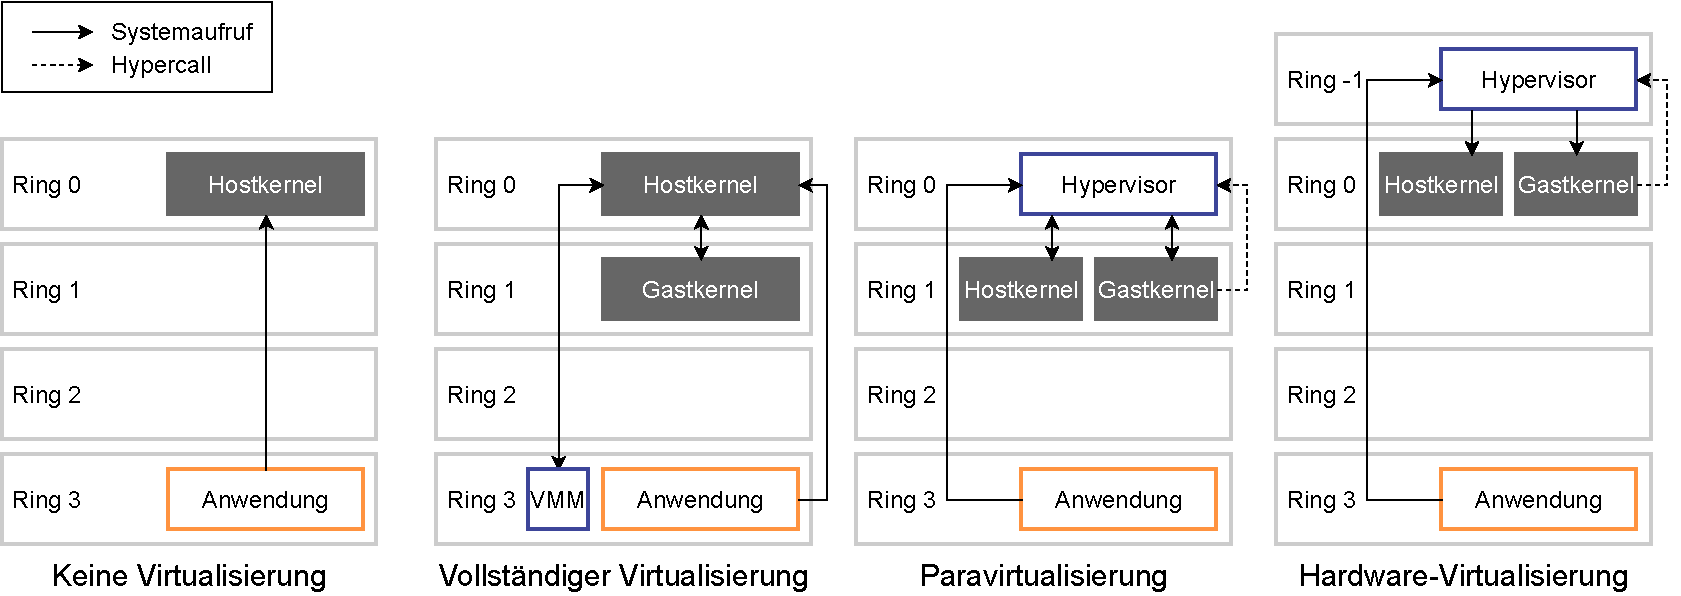
\includegraphics[width=1\linewidth]{gfx/virtualiserung.pdf}
	\caption{Virtualisierung im Vergleich}
	\footnotesize Quelle: In Anlehnung an \cite[vgl.][236, 238, 240]{Baun.2017}
	\label{fig:virtualiserung}
\end{figure} 

\section{Kernel-based Virtual Machine}
\label{sec:kvm}
\ac{KVM} ist eine Virtualisierungslösung mit der Architektur einer vollständigen Virtualisierung und unterstützt Hardware-Virtualisierung . \ac{KVM} ist seit 2007 Teil des Linuxkernels \cite[vgl.][8]{Peichert.20150928}. Neben \ac{KVM} existieren auch andere Produkte, wie beispielsweise VMware \cite[vgl.][237]{Baun.2017}. \ac{KVM} findet bei den in dieser Thesis betrachteten Technologien Verwendung und wird daher hier erläutert.
Bei \ac{KVM} lädt der Kernel beim Starten das benötigte Kernelmodul nach und ermöglicht den Betrieb von nahezu jedem Gastsystem. Wenn das Gastsystem mit \ac{QEMU} kompatibel ist, kann \ac{KVM} das Gastsystem mit sehr geringen Performanzverlusten ausführen. Wenn das System nicht kompatibel ist, emuliert \ac{QEMU} die Hardware. Diese Emulation ist deutlich langsamer \cite[vgl.][8]{Peichert.20150928}.

\section{Container}
\label{sec:container}
Container sind vergleichbar mit virtuellen Maschinen: Auch hier werden Anwendungen gekapselt auf einem System betrieben. Die Softwareschicht zwischen realem Computer und der Anwendung, die isoliert ausgeführt wird, ist gegenüber einer \ac{VM} deutlich reduziert. Beim Betrieb von Anwendungen in Containern sinken die Infrastrukturkosten gegenüber \acp{VM}, da viele Redundanzen wegfallen. Die Firma Docker nennt in einem Beispiel für Docker Container eine Reduktion um 66\% \cite[vgl.][]{BettyJunod.2017}.

Baun definiert Container-Virtualisierung im Artikel Servervirtualisierung folgendermaßen: "`Hier laufen unter ein und demselben Betriebssystemkern mehrere voneinander abgeschottete identische Systemumgebungen. Es wird kein zusätzliches Betriebssystem, sondern eine isolierte Laufzeitumgebung virtuell in einem geschlossenen Container erzeugt."' \cite[203]{Baun.2009}
Der Grafik \ref{fig:vmcontainer} sind die unterschiedlichen Schichten in den Architekturen von Containern und virtuellen Maschinen zu entnehmen.

Dabei werden die Kernel Funktionen Namespaces und Control Groups verwendet, um diese Applikationen voneinander zu isolieren \cite[vgl.][4]{Scholl.2019}.
Ein Container wird immer aus einem Containerabbild, dem Container Image, gestartet das einer Vorlage entspricht. Die Ausführung des Containers übernimmt dabei die Container Runtime. Damit ist, eine entsprechende Vorlage vorausgesetzt, eine Anwendung in einem Container in unter einer Minute betriebsbereit. Die Containerabbilder liegen in einem Standardformat vor. \cite[vgl.][S. 240 f.]{Baun.2017}
Dieses Format hat die \ac{OCI} in der "`Image Format Specification"' \cite[vgl.][]{OpenContainerInitiative.} festgelegt. Jede Software, welche die "`Runtime Specification"'  \cite[vgl.][]{OpenContainerInitiative.20200205} implementiert, ist dann in der Lage einen Container nach \ac{OCI} Spezifikation auszuführen \cite[vgl.][]{FerdinandThommes.20170720}.
Damit werden die Abhängigkeiten zur Ausführung eines Containers minimiert. Ein Container lässt sich, wie sein Vorbild in der Realität, einfach umziehen und fast überall starten \cite[vgl.][15]{Jangla.2018}. 

Die Unveränderlichkeit des Images hat verschiedene Auswirkungen: Bei der Inbetriebnahme eines Containers aus dem gleichen Image wird immer das gleiche Ergebnis entstehen. Damit ist es reproduzierbar. Auch werden alle Änderungen, die zur Laufzeit stattfinden, genau im Container gespeichert. Diese Änderungen lassen sich anzeigen, sodass sich ungeplante Änderungen oder Angriffe nachvollziehen lassen.
Ein Container speichert Daten nicht persistent, daher sind diese nach einem Containerneustart nicht mehr vorhanden. Mit Volumes können Daten im Container persistent gespeichert werden. Dazu wird ein Ordner auf dem Host-System an den Container weitergereicht und eingebunden.  \cite[vgl.][4]{Felter.2015}

\begin{figure}[hb]
	\centering
	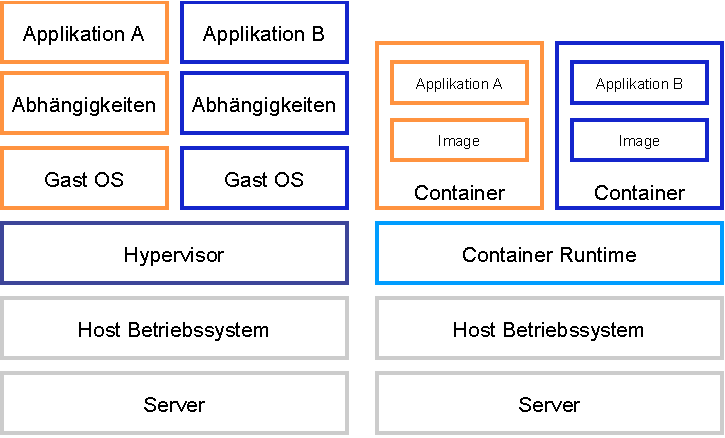
\includegraphics[width=1\linewidth]{gfx/vm_container.pdf}
	\caption{Virtuelle Maschine und Container im Vergleich}
	\label{fig:vmcontainer}
\end{figure}


\section{Docker}
\label{sec:docker}
Docker ist eine Entwicklerplattform für Container-Virtualisierung und wurde 2013 von der Docker Inc. veröffentlicht \cite[vgl.][10]{Jangla.2018}. Der Fokus von Docker liegt auf der Erstellung, Ausführung und Bereitstellung von Applikationen mithilfe von Containern \cite[vgl.][11]{Jangla.2018}.
Über den Docker Client wird die Docker Engine angesprochen. Durch diese Architektur kann ein Docker Client auf System A Container in der Docker Engine auf System B verwalten \cite[vgl.][55]{Poulton.2017}.
Die Docker Engine besteht dabei aus dem Docker daemon, containerd, Shim und der Runtime runc. Diese Bestandteile haben sich aus einem Docker daemon entwickelt. Die Trennung wurde vorgenommen, um die Entwicklung besser zu steuern und um Teile der Architektur tauschen zu können \cite[vgl.][55]{Poulton.2017}. 
Dabei stellt der Daemon die Schnittstellen bereit, um zwischen Docker Client und containerd zu kommunizieren. Die Kommunikation zwischen Client und Daemon erfolgt via REST API, die zwischen  Daemon und containerd via gRPC \cite[vgl.][60]{Poulton.2017}. 
Containerd ist für die Verwaltung der Container zuständig, dabei delegiert er an die Runtime. Containerd übergibt zum Beispiel das Image an runc \cite[vgl.][59]{Poulton.2017}. Containerd unterstützt dabei alle \ac{OCI} kompatiblen Runtimes und Images, vgl. \ref{sec:container}. Die Komponente Shim, englisch für Unterlegscheibe, fungiert als Entkopplung von Containerbetrieb und Administration. Dadurch lässt sich zum Beispiel eine Aktualisierung des Docker Daemons vornehmen, ohne dass der Betrieb der Container eingeschränkt wird  \cite[vgl.][S. 62 f.]{Poulton.2017}. Die Runtime runc ist für den eigentlichen Betrieb des Containers zuständig und leitet die Systemaufrufe aus dem Container an den Host Kernel weiter \cite[vgl.][59]{Poulton.2017}. Einen Überblick über die Architektur gibt die Abbildung \ref{fig:docker}.
Im weiteren Verlauf der Arbeit wird Docker häufig als Container Runtime bezeichnet, auch wenn die eigentliche Runtime runc ist. Dies dient der sprachlichen Vereinfachung und es ist in diesem Zusammenhang immer runc gemeint.

Docker nutzt verschiedene Linux-Funktionen, um die Container zu isolieren: Namespaces sorgen dafür, dass die Prozesse in einzelnen Containern, zueinander und zum Host System getrennt sind. Dadurch hat zum Beispiel jeder Netzwerk Namespace eine eigene IP-Adresse und ein eigenes Netzwerkinterface oder jeder Prozess seinen eigenen Prozessbaum. Docker verwendet Namespaces für die Isolierung von Prozessen, dem Netzwerk, Mounts, Inter-Prozess-Kommunikation, Nutzern und Hostnamen \cite[vgl.][S. 171 f.]{Poulton.2017}. In dem Buch "`Docker deep dive"' bezeichnet der Autor "`Container als organisierte Sammlung von Namespaces"'\footnote{Übersetzt aus: "`container is an organized collection of namespaces"' \cite[][172]{Poulton.2017}} \cite[][172]{Poulton.2017}.
Control Groups limitieren die Prozesse im Container. Damit ist eine Beschränkung der Nutzung von CPU, RAM und I/O möglich \cite[vgl.][172]{Poulton.2017}. Standardmäßig hat ein Docker Container keine Beschränkungen \cite[vgl.][]{DockerInc.2020}.
Mit Capabilities ist es möglich, einen Prozess in einem Container als nicht-root auszuführen, bestimmte Rechte, die eigentlich root voraussetzen, aber zu erlauben. Damit kann ein Container zum Beispiel bestimmte Netzwerkports verwenden \cite[vgl.][173]{Poulton.2017}.
Zusätzlich ist es möglich die Systemaufrufe durch runc mit Seccomp zu filtern. Im default Seccomp Profil sind 44 Systemaufrufe geblockt \cite[vgl.][]{DockerInc..20191203}. Seccomp, für "`secure computing"', ist eine Funktion des Linux Kernels, die Prozesse davon abhält bestimmte Systemaufrufe zu verwenden. Es sind nur die Aufrufe erlaubt, die im Seccomp Profil aufgeführt sind \cite[][S. 12 f.]{Randal.28.04.2019}.

Zunächst lief Docker nur auf Unix Systemen, seit Ende 2016 ist es auch mit Windows kompatibel \cite[vgl.][11]{Jangla.2018}. Dabei lassen sich unter Linux nur Linux Container und auf Windows entweder Linux oder Windows Container ausführen. Ein Mischbetrieb unter Windows ist nicht möglich \cite[vgl.][]{cwilhit.2019}. Dabei wird beim Betrieb eines Linux Containers unter Windows eine virtuelle Maschine gestartet, um den Linux Kernel in der \ac{VM} für die Containerausführung zu verwenden \cite[vgl.][28]{Poulton.2017}.

\begin{figure} [ht]
	\centering
	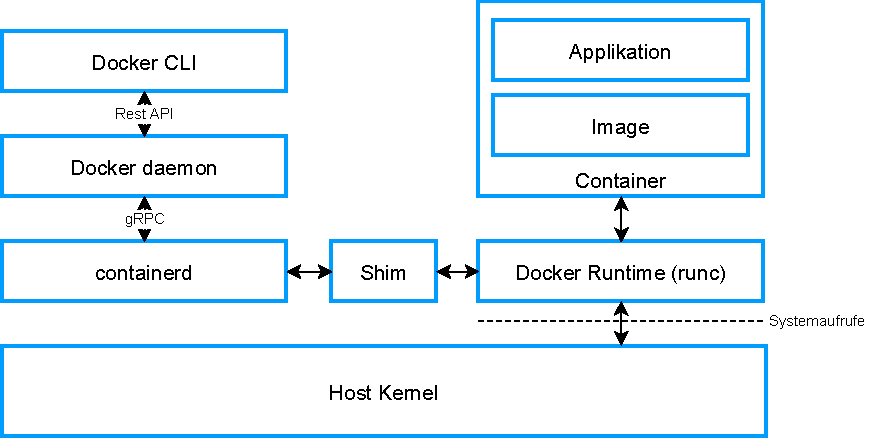
\includegraphics[width=1\linewidth]{gfx/docker_arch.pdf}
	\caption{Architektur von Docker}
	\label{fig:docker}
\end{figure}

\section{Docker Image}
Docker startet seine Container von Docker-Images aus. Ein Docker-Image ist eine Reihe von Datenschichten über einem Basis-Image. Die meisten Docker-Images starten von einem Basis-Image, wie zum Beispiel einem Ubuntu-Basis-Image \cite[vgl.][]{Ubuntu.20200220} oder Alpine-Basis-Image \cite[vgl.][]{Alpine.20200220}. 

Um mit mehreren Schichten eines Images eine einzige Dateisystemschicht zu bearbeiten, verwendet Docker ein spezielles Dateisystem namens Union File System. Dieses ermöglicht Dateien und Verzeichnisse in verschiedenen Dateisystemen zu einem einzigen konsistenten Dateisystem zusammenzufassen. \cite[vgl.][3]{Bui.13.01.2015}
Wenn Benutzer Änderungen an einem Container vornehmen, fügt Docker, anstatt die Änderungen direkt in das Abbild des Containers zu schreiben, eine zusätzliche Ebene hinzu, die diese Änderungen an dem Abbild enthält. Wenn der Benutzer beispielsweise MySQL in ein Ubuntu-Image installiert, erstellt Docker eine Datenschicht, die MySQL enthält und fügt dann dem Image eine weitere Schicht hinzu. Dieser Prozess macht den Image-Verteilungsprozess effizienter, da nur die aktualisierten Datenschichten verteilt werden müssen.

Die Docker Images werden in der Regel in einer Datenbank, einer Registry, vorgehalten, damit sie für die Ausführung eines Containers nicht neu erzeugt werden müssen \cite[vgl.][91]{Scholl.2019}. Dazu beherrschen die Container Runtimes häufig das Hoch- und Herunterladen von Container Images aus einer solchen Datenbank. Für diesen Prozess hat die Open Container Initiative einen Standard festgelegt, die "`Distribution Specification"' \cite[vgl.][]{HansJoachimBaader.20180410, OpenContainerInitiative.20200212}.

\section{Kubernetes}

Kubernetes ist eine Software, die zur Orchestrierung von Containern entwickelt und von Google 2014 veröffentlicht wurde  \cite[vgl.][7]{Scholl.2019}. Dabei bildet Kubernetes ein verteiltes System über alle Hosts des Kubernetes Clusters. Dadurch können Container, je nach Rechenlast, zwischen den einzelnen Host umverteilt werden, die Container skaliert oder die Kommunikation zwischen Containern auf verschiedenen Hosts sichergestellt werden \cite[vgl.][4]{Bernstein.2014}.
Derzeit ist Kubernetes die verbreitetste Orchestrierungslösung für Container \cite[vgl.][6]{sysdig.2019}.
Kubernetes unterstützt alle \ac{OCI} kompatiblen Runtimes für den Container Betrieb 
\cite[vgl.][7]{Scholl.2019}.

\section{Stand der Technik}
Ein Ansatz für die Absicherung von Container-Virtualisierung ist die Erhöhung der Isolierung. Dies kann durch verschiedene Herangehensweisen erreicht werden. Eine Möglichkeit ist Container in virtuellen Maschinen zu betreiben, eine andere die Container mit einem Kernel im Userspace zu verwenden. Weiter ist es möglich, Container in Unikernels einzusetzen. Für jede dieser Methoden wird in im Folgenden eine Lösung vorgestellt.
Die Grafik \ref{fig:zeitstrahl_vm_container} gibt einen Überblick über die Entstehung von vielen in der vorliegenden Arbeit benannten Technologien. Die genannten Begriffe sind im Zeitstrahl für die bessere Übersicht markiert.

\begin{figure}[hb]
	\centering
	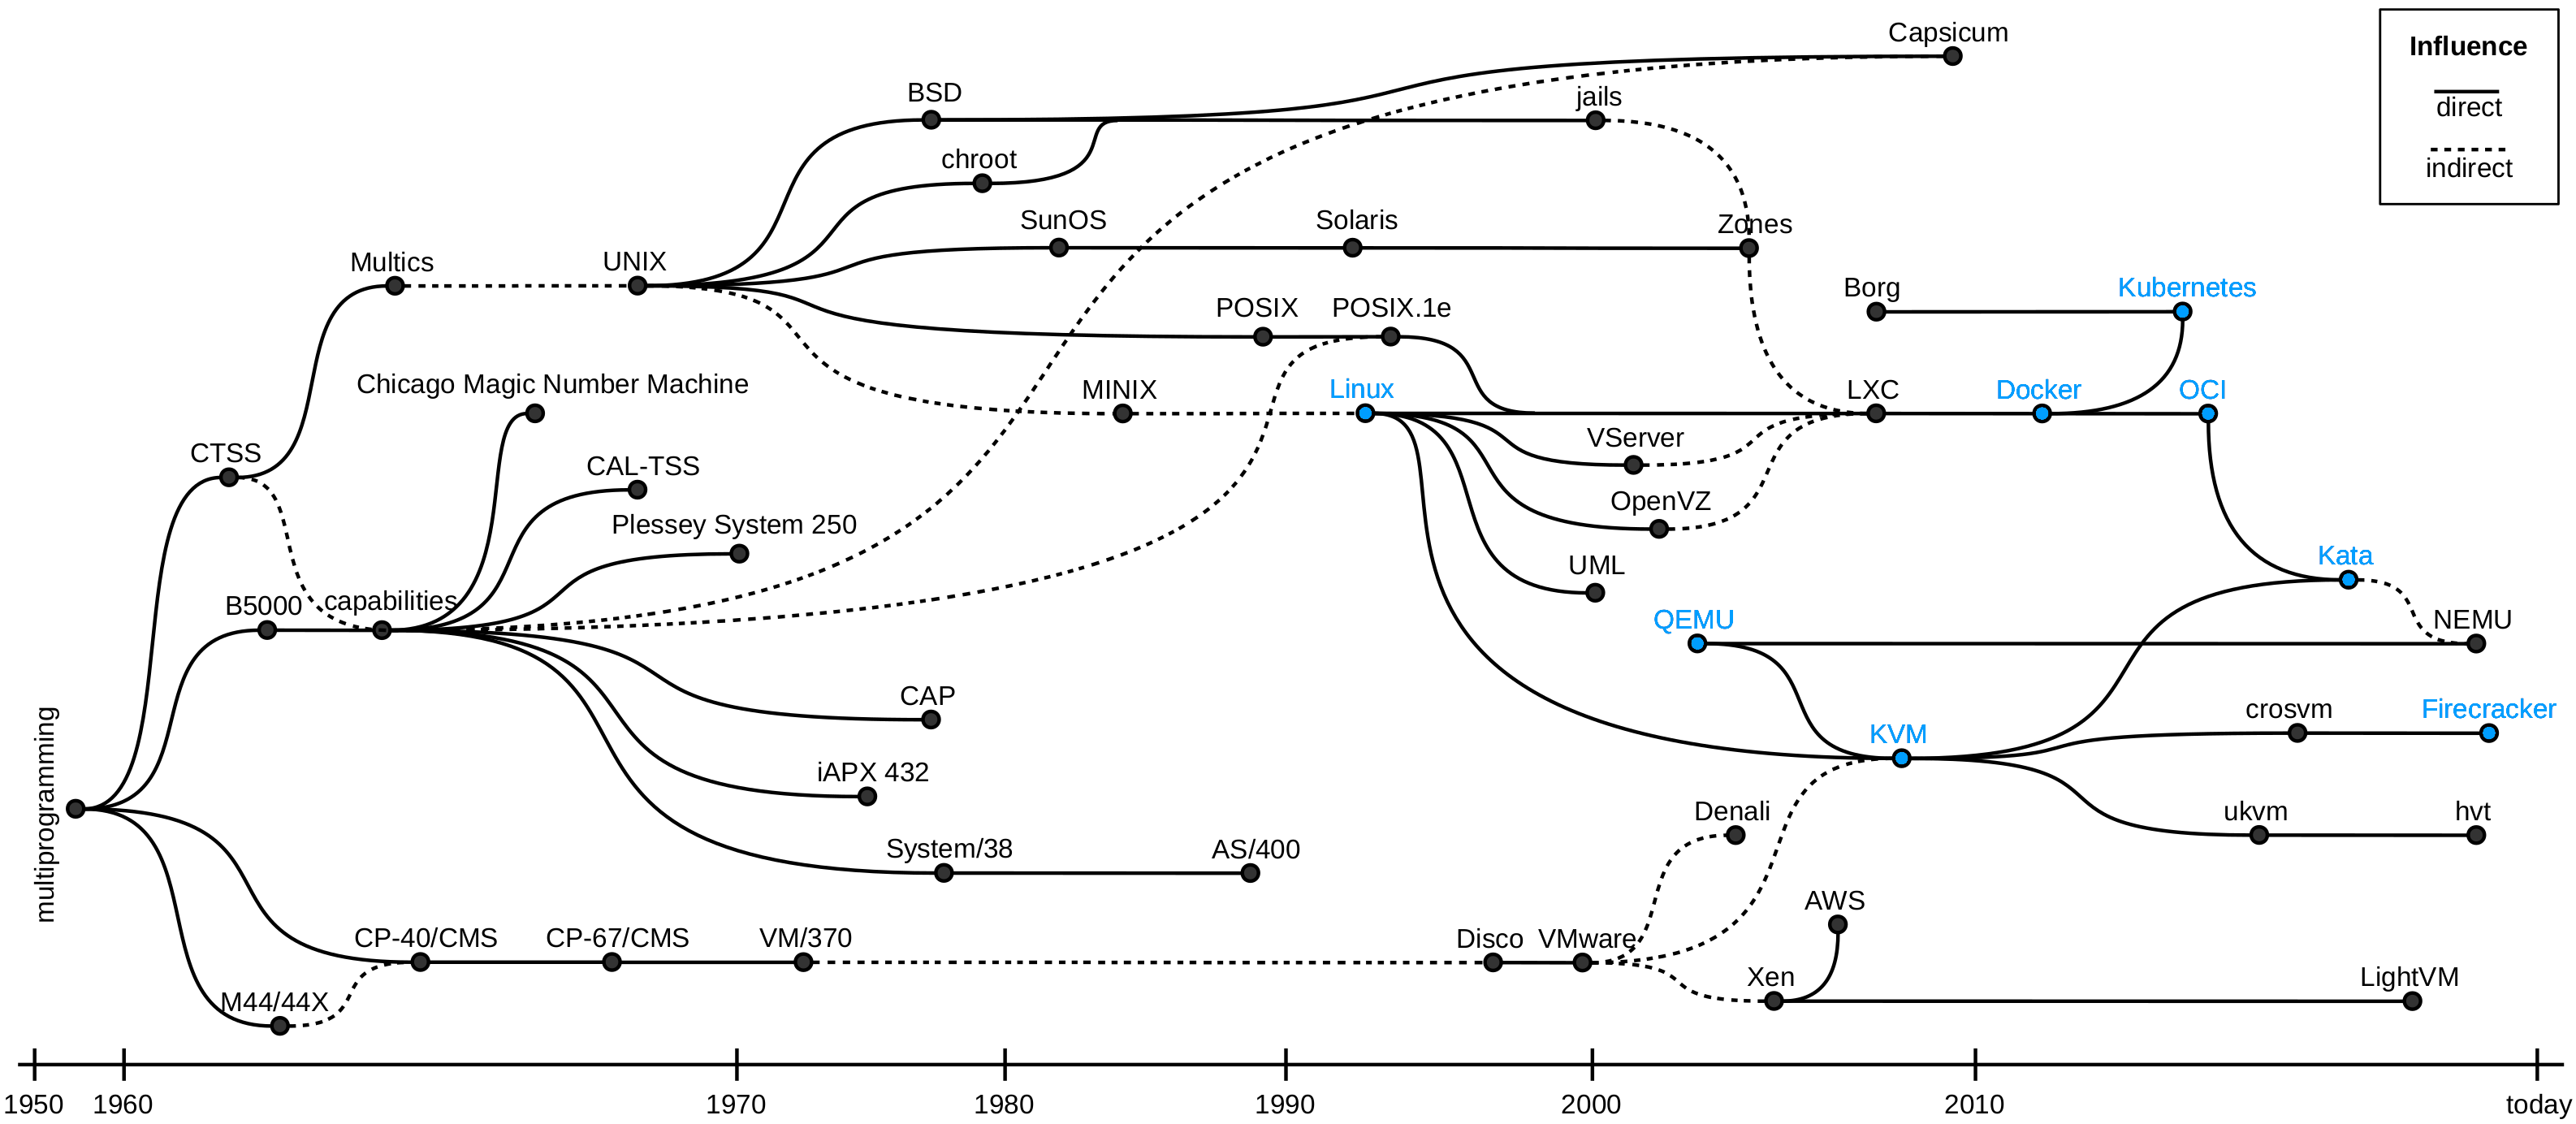
\includegraphics[width=1\linewidth]{gfx/VM_Container_Zeitstrahl.png}
	\caption{Die Entwicklung von Virtualisierung und Containern} 
	\footnotesize Quelle: In Anlehnung an \cite[][2]{Randal.28.04.2019}
	\label{fig:zeitstrahl_vm_container}
\end{figure}
\newpage

\subsection{Kata Containers}
\label{sec:kata}
Kata vereint die Isolierung von virtuellen Maschinen mit der unkomplizierten Nutzung von Containern \cite[vgl.][28]{TamHanna.01.11.2019}. Kata Container basiert auf den Technologien Hyper.sh und Intel’s clear containers  \cite[vgl.][6]{Scholl.2019}. Im Mai 2018 wurden diese beiden Projekte zusammengeführt und als Kata Containers veröffentlicht. Betreut wird das Projekt von der Open-Stack Foundation \cite[vgl.][106]{UdoSeidel.2018}.

Die Grundlage für die Virtualisierung bildet \ac{QEMU}, das auch in der Virtualisierung \ac{KVM} verwendet wird, vgl. \ref{sec:kvm}. Für jeden einzelnen Container startet Kata eine \ac{VM} \cite[vgl.][107]{UdoSeidel.2018}. Als Betriebssystem der virtuellen Maschine kommt Clear Linux zum Einsatz. Dieses Linux wurde von Intel auf Container optimiert und zielt auf einen möglichst geringen Ressourcenverbrauch ab  \cite[vgl.][107]{UdoSeidel.2018}. Da Kata \ac{QEMU} verwendet wird ein System mit Hardware-Virtualisierung vorausgesetzt  \cite[vgl.][108]{UdoSeidel.2018}.
Kata Containers beinhaltet auch eine \ac{OCI} kompatible Runtime, die sich neben der Runtime von Docker verwenden lässt \cite[vgl.][107]{UdoSeidel.2018}. Dadurch dass Docker die Container Runtime Schnittstelle nach dem Standard der \ac{OCI} implementiert hat, war es den Kata Entwicklern möglich, Kata in Docker zu integrieren \cite[vgl.][28]{TamHanna.01.11.2019}.
 
Damit eine Verwaltung des Containers in der \ac{VM} vom Host aus möglich ist, muss der Container für die Runtime, in diesem Fall kata-runtime, transparent sein. Dafür stellt Kata einen Shim bereit. Die Hauptaufgabe des Shims ist es, die I/O Verbindungen des Containers zu verwalten \cite[vgl.][]{katacontainers.20191207}. Dies wird mit den weiteren Elementen Proxy und Agent erreicht. Sie kommunizieren über die serielle Schnittstelle von \ac{QEMU} miteinander. Der Agent ist ein Prozess innerhalb der \ac{VM}. Pro \ac{VM} wird als Gegenstück auf dem Host ein Proxy gestartet. Die Abbildung \ref{fig:kata} verdeutlicht diese Architektur \cite[vgl.][107]{UdoSeidel.2018}.

Neben der Integration in Docker ist Kata Containers auch mit Kubernetes kompatibel. Es ist möglich, Kata und Docker parallel in einem Kubernetes Cluster zu betreiben und je nach Anwendung eine der Runtimes zu verwenden  \cite[vgl.][]{katacontainers.20191207}.
Die Entwickler stellen für viele Linux Distributionen Pakete zu Verfügung, mit denen sich Kata installieren lässt \cite[vgl.][]{katacontainers.20200120}. Weiter ist es auch möglich, Kata selbst zu kompilieren \cite[vgl.][108]{UdoSeidel.2018}.

\subsection{Kata Containers - Firecracker}
\label{sec:katafc}
Firecracker ist ein virtueller Maschinenmonitor, vgl. \ref{sec:virtualiserung}, der auf \ac{KVM} läuft, vgl. \ref{sec:kvm}. 
In der \ac{VM} wird ein minimaler Firecracker Kernel gebootet. Dieser hat eine sehr reduzierte Hardware Unterstützung. Für das Netzwerk Interface und den Zugriff von Daten sind bisher virtio net und virtio block implementiert \cite[vgl.][]{ArunGupta.2018}. Dadurch ist der Kernel besonders klein \cite[vgl.][11]{Randal.28.04.2019}. Für den Hersteller Amazon stand Geschwindigkeit, Sicherheit und Leichtgewichtigkeit im Fokus der Entwicklung \cite[vgl.][]{ArunGupta.2018}.

Kata Containers veröffentlichte mit der Version 1.5 die Unterstützung von Firecracker als Hypervisor. Dabei wird Firecracker anstelle von \ac{QEMU} verwendet, dies soll die Komplexität und den Ressourcenverbrauch verringern \cite[vgl.][11]{Randal.28.04.2019}.
Kata mit Firecracker, kurz Kata FC, ist zu Docker und Kubernetes kompatibel. Einige Funktionen wie die Verwendung von Ressourcenlimits, die Unterstützung von Container Volumes und Speicher Typen neben Block Speichern, fehlen bisher \cite[vgl.][]{katacontainers.20190123}. 

\begin{figure}[ht]
	\centering
	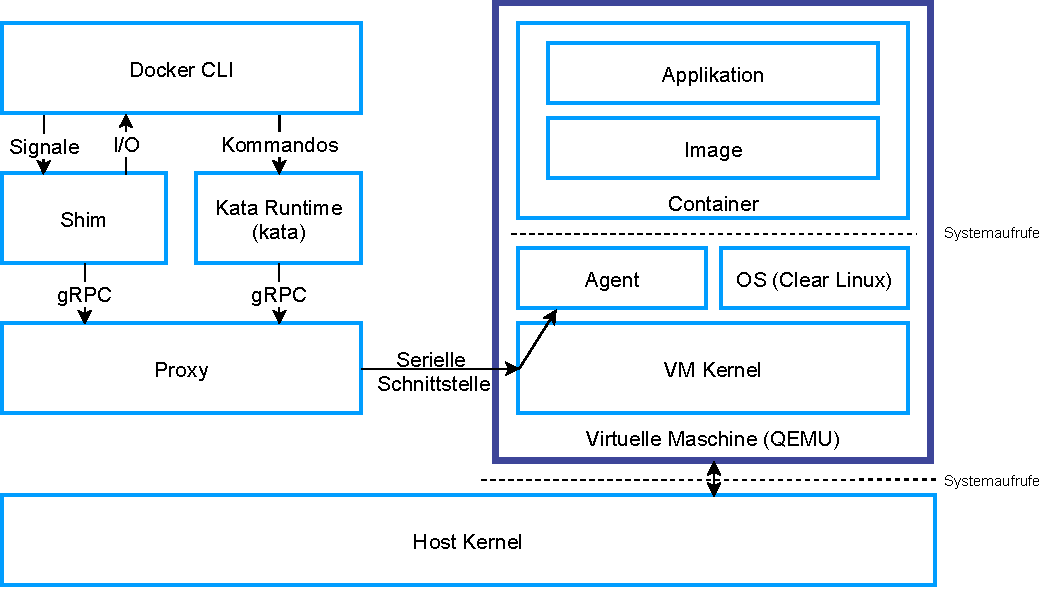
\includegraphics[width=1\linewidth]{gfx/kata_arch.pdf}
	\caption{Architektur von Kata Containers}
	\footnotesize Quelle: In Anlehnung an \cite[vgl.][ab 12:35]{NilsMagnus.20190425}
	\label{fig:kata}
\end{figure}

\subsection{gVisor}
\label{gvisor}
gVisor ist eine Container Runtime und ein an den Linux Kernel angelehnter Kernel im Userspace \cite[vgl.][6]{Scholl.2019}. 
Die Hauptbestandteile bilden Sentry und Gofer. Sentry beinhaltet den Kernel und läuft auf Linux. Gofer ist ein Proxy für die Dateiverarbeitung, der die Informationen dann an Sentry weiterleitet. Für die Kommunikation wird das Protokoll 9P verwendet \cite[vgl.][108]{UdoSeidel.2018}.
Die Abbildung \ref{fig:gvisor} veranschaulicht die Architektur von gVisor und verwendet die Datengrundlage aus der Arbeit "`The True Cost of Containing: A gVisor Case Study"' \cite[vgl.][]{EthanG.Young.2019}.

Sentry hat zwei Modi für die Verarbeitung von Systemaufrufen. Dabei werden im ptrace Modus Systemaufrufe unterbrochen und im \ac{KVM} Modus als Gast in einer \ac{VM} ausgeführt \cite[vgl.][2]{EthanG.Young.2019}.
Der Standardmodus ist ptrace, dies kann bei sehr rechenintensiven Aufgaben zu Performanzeinbußen führen. In solchen Fällen sollte die Verwendung von \ac{KVM} als gVisor Plattform zu einer Leistungssteigerung führen. Dies ist nur auf Systemen möglich, die Hardware-Virtualisierung unterstützen. \ac{KVM} als Plattform ist noch experimentell \cite[vgl.][109]{UdoSeidel.2018}.

Applikationen, die auf Sentry laufen, können laut Ethan Young 211 von den 319 Systemaufrufen unter Linux verwenden \cite[vgl.][2]{EthanG.Young.2019}. In der Systemaufrufkompatibilitätsreferenz von gVisor sind 166 Aufrufe als voll unterstützt markiert \cite[vgl.][]{gVisor.20200122}. Ein anderer Autor weist darauf hin, dass die implementierten Aufrufe dem Quellcode in der Datei "`gvisor/pkg/sentry/syscalls/linux/linux64.go"' zu entnehmen sind \cite[vgl.][108]{UdoSeidel.2018}.

Dabei nutzt Sentry für die Implementierung dieser Aufrufe selbst nur 55, die an den Host Kernel weitergegeben werden. Seccomp Filter verhindern, dass ein kompromittierter Sentry andere als diese 55 Systemaufrufe  verwendet.
Nach den gVisor Entwicklern werden die Aufrufe open und socket für die meisten Angriffe verwendet, um aus einem Container auszubrechen. Daher sind diese auch nicht unter den 55 erlaubten Aufrufen und die gVisor Bestandteile für den Netzwerk- und Speicherzugriff verzichten auf diese Systemaufrufe. \cite[vgl.][2]{EthanG.Young.2019}

\begin{figure}[hb]
	\centering
	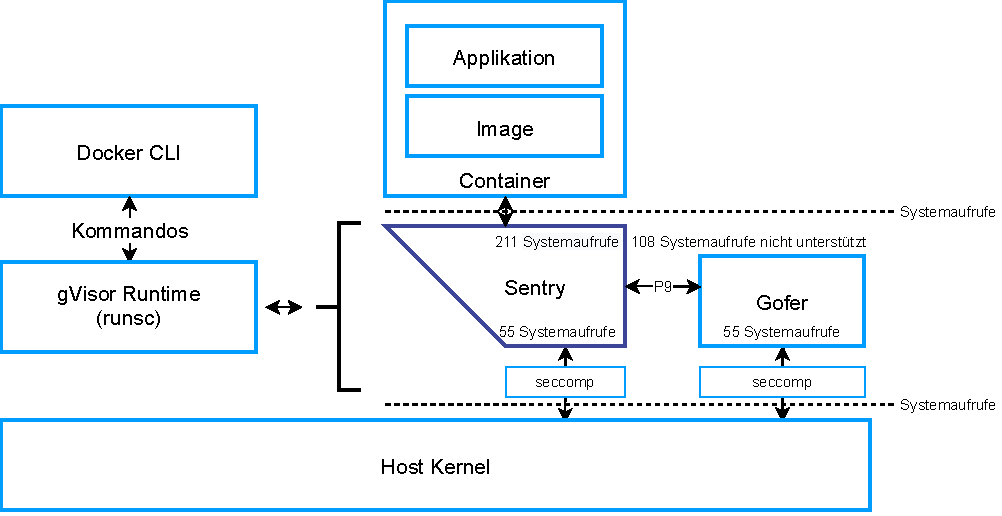
\includegraphics[width=0.9\linewidth]{gfx/gVisor_arch.pdf}
	\caption{Architektur von gVisor} 
	\footnotesize Quelle: In Anlehnung an \cite[][2]{EthanG.Young.2019}
	\label{fig:gvisor}
\end{figure}

Um die Angriffsvektoren in Bezug auf die Arbeit mit Dateien zu minimieren, wurden laut Young drei wichtige Muster implementiert: "`Erstens implementiert gVisor intern mehrere Dateisysteme [...]. Sentry kann in der Regel diese internen Dateisysteme verarbeiten, ohne den Host Kernel oder andere Helfer aufzurufen. Zweitens öffnen die Sentry-Dienste Aufrufe an externen Dateien [...] mithilfe von Gofer [...]; Gofer ist in der Lage, Dateien im Namen des Sentry zu öffnen und sie über einen 9P Kanal zurückzugeben. Drittens kann der Sentry, nachdem er ein Handle für eine externe Datei hat, Systemaufrufe aus der Anwendung lesen und schreiben, indem er ähnliche Systemaufrufe an den Host sendet.\footnote{Übersetzt aus: "`First, gVisor implements several file systems internally [...]; the Sentry can generally serve I/O to these internal file systems without calling out to the host or other helpers. Second, the Sentry services open calls to external files [...] with the help of [...] Gofer; the Gofer is able to open files on the Sentry’s behalf and pass them back via a 9P (Plan 9) channel. Third, after the Sentry has a handle to an external file, it can serve read and write system calls from the application by issuing similar system calls to the host."' \cite[][2]{EthanG.Young.2019}}"' \cite[][2]{EthanG.Young.2019}

Durch die eigene Implementierung des Kernels und den Verzicht auf einige Systemaufrufe ist gVisor nicht mit jeder Anwendung kompatibel. In der Dokumentation ist der jeweilige Implementationsstatus für jeden Systemaufruf ersichtlich \cite[vgl.][]{gVisor.20200122}. Eine Übersicht über getestet Anwendungen, die fehlerfrei laufen, ist der Dokumentation zu entnehmen \cite[vgl.][]{gVisor.20191025}.
Durch die Einhaltung der \ac{OCI} Standards ist die Runtime (runsc) von gVisor einfach mit Docker oder Kubernetes zu verwenden \cite[vgl.][108]{UdoSeidel.2018}.



\subsection{Nabla Containers}
\label{nabla}
Nabla Containers, kurz Nabla, erreicht eine hohe Isolierung durch die Filterung von Systemaufrufen vom Container Kernel zum Host Kernel \cite[vgl.][14]{Randal.28.04.2019}. Dabei basiert Nabla auf einem Unikernel, konkret wird Rumprun verwendet.
Ziel des Rumprun Projektes ist es, bestehende POSIX Anwendungen als Unikernel auf Hypervisoren auszuführen \cite[vgl.][256]{Jaworski.2020}.

Die Filterung wird durch seccomp in Kombination mit Solo5 vorgenommen. Erlaubt sind die folgenden sieben Systemaufrufe: read, write, ppoll, exit\_group, clock\_gettime, pwrite64 und pread6  \cite[vgl.][109]{UdoSeidel.2018}. Solo5 ist ein Portierung des Unikernels MirageOS auf \ac{KVM} \cite[vgl.][4]{Williams.2016}. Solo5 ist damit ein Bestandteil der Nabla Runtime und übernimmt die Systemaufruffilterung. Zusätzlich stellt es ein Interface bereit, auf dem Rumprun ausgeführt wird. Die Abbildung \ref{fig:nabla} veranschaulicht diese Architektur  \cite[vgl.][]{Nablacontainers.20190501}. 

Nabla verwendet zwei verschiedene Unikernels, um die Anwendung auszuführen und auf dem Host zu betreiben.
Eine Anwendung, die in einem Nabla Container ausgeführt werden soll, wird mit dem Rumprun Kernel zu einem ausführbaren Binary vereint. Dabei ist in einem solchen System nur eine Datei ausführbar. Dies ist nur möglich, wenn die Anwendung auf Rumprun lauffähig ist. Diese Einheit wird dann auf Solo5 ausgeführt \cite[vgl.][S. 109 f.]{UdoSeidel.2018}. 

Nabla hat die Projekte Solo5 und Rumprun geforked und an ihre Bedürfnisse angepasst. Dadurch sind nicht alle portierten Anwendungen für den ursprünglichen Rumprun Kernel mit Nabla kompatibel  \cite[vgl.][S. 109]{UdoSeidel.2018}.
Die Nabla Runtime (runnc) ist \ac{OCI} kompatibel, kann also mit Docker verwendet werden. Images nach dem \ac{OCI} Standard lassen sich aber nicht verwenden \cite[vgl.][S. 5 f.]{Scholl.2019}. 
Derzeit werden Container Volumes, Ressoucen Limits oder das Schreiben von Dateien außerhalb von /tmp noch nicht unterstützt  \cite[vgl.][]{nablacontainers.20190402}.

\begin{figure}[hb]
	\centering
	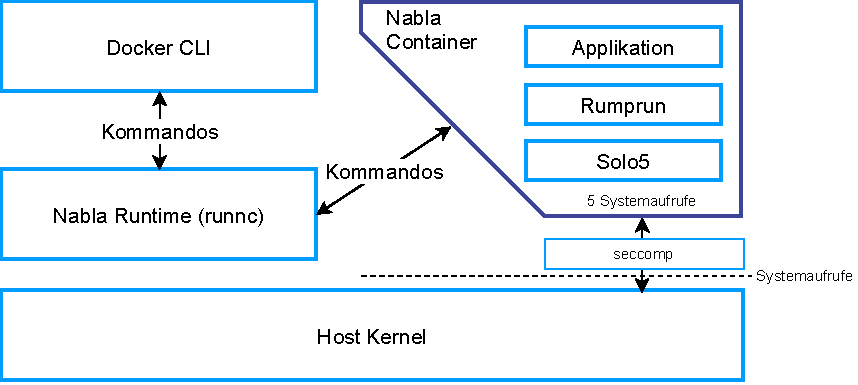
\includegraphics[width=1\linewidth]{gfx/nabla_arch.pdf}
	\caption{Architektur von Nabla}
	\label{fig:nabla}
\end{figure}

\section{Related Work}
\label{sec:relatedwork}

Der Autor Tam Hanna vergleicht Kata Containers mit Docker. Er bewertet Kata als sicherer, da es zur Ausführung ein virtuelles System verwendet. Weiter betrachtet er die Startzeit von Containern, die Antwortzeiten in einem Netzwerk und den Arbeitsspeicherverbrauch. In allen Disziplinen schneidet Kata schlechter ab als Docker. Die Messungen sind aber nur bedingt aussagekräftig, da diese kaum wiederholt werden und auch die unterschiedlichen Ressourcenlimits der Kandidaten nicht beachtet werden. \cite[vgl.][]{TamHanna.01.11.2019}

Im genannten Artikel wird die I/O Messung des Blogs stackhpc.com erwähnt. In diesem Beitrag wird die I/O Leistung auf einem Netzlaufwerk von einem echten Server, Docker und Kata betrachtet. Dabei ist Docker dem Server fast ebenbürtig, während Kata meist 15\% der Serverleistung erzielt. Die Latenz für das Schreiben oder Lesen von Dateien ist bei Docker und Kata signifikant schlechter, als die des Servers. \cite[vgl.][]{BharatKunwar.09.05.2019}

Die Kata Entwickler Xu Wang und Fupan Li vergleichen in einem Konferenzvortrag Kata und gVisor. Dabei verwendet der \ac{QEMU} Prozess in Kata weniger Systemaufrufe als gVisor. Der Verbrauch des Arbeitsspeichers ist bei Kata deutlich höher. Bei der Betrachtung der Startzeiten eines Containers liegt gVisor klar vor Kata und ist auch schneller als Docker. Der Vergleich der CPU Leistung zwischen Host, Kata und gVisor zeigt nur geringe Unterschiede. Der Overhead beim Schreiben in den Arbeitsspeicher ist bei Kata zwischen 2,5\% und 8\% und bei gVisor zwischen 5,5\% und 13\%. Die Ergebnisse im I/O Vergleich decken sich mit denen von \cite{BharatKunwar.09.05.2019}, wobei Kata mit aktiviertem "`passthru fs"' deutlich bessere Ergebnisse erzielt. gVisor ist beim Schreiben von 128 KB großen Dateien schneller als Kata, bei Dateien von 4 KB gleichauf. Zusammenfassend startet gVisor schneller und hat einen geringeren RAM Verbrauch. In fast allen anderen Disziplinen ist Kata schneller. \cite[vgl.][]{XuWang.2018}

In der Arbeit "`The True Cost of Containing: A gVisor Case Study"' wird gVisor mit Docker verglichen. gVisor ist sicherer als Docker, da bei einer Kompromittierung nur Sentry, ein Prozess im Userspace, und nicht der Host Kernel betroffen sei. Dabei ist gVisor deutlich langsamer. Im Detail ist Docker bei Systemaufrufen, Speicherzuweisungen und bei große Downloads mehr als doppelt so schnell und beim Öffnen von Dateien sogar über 200 mal schneller. \cite[vgl.][]{EthanG.Young.2019}

Der IBM Mitarbeiter James Bottomley vergleicht in einem Blog Beitrag Docker, Kata, gVisor und Nabla. Um die Leistung zu vergleichen, verwendet er die Antworten pro Sekunde von Redis, Python Tornado und Node Express. Docker erreicht den höchsten Durchsatz, gVisor den Niedrigsten. Kata und Nabla liegen dazwischen \cite[vgl.][]{JamesBottomley.14.07.2018}.
Zusätzlich führt er zu Bewertung der Sicherheit einer Container Runtime eine eigene Methode ein, das sogenannte "`Horizontal Attack Profile"'. Diese quantitative Methode misst die Codemenge im Linux Kernel, die vom laufenden System durchlaufen wird. Er nimmt an, dass die Fehlerdichte im Kernel gleich verteilt ist und je mehr Code ein Programm ausführt, desto mehr Programmierfehler sind potenziell ausnutzbar. Damit wäre ein Programm, das wenig Code im Kernel ausführt sicherer, als eines das viel Code ausführt. Dabei ist die Messung bei Containern mit dem Kernel Werkzeug ftrace unkomplizierter als bei Hypervisoren oder \ac{VMM}. Bei der Messung wird die Anzahl der aufgerufenen Funktionen, nicht die der durchlaufenen Codezeilen erhoben.
Nach dieser Methode ist Nabla deutlich sicherer als Docker. Kata und gVisor verwenden fast genauso viele Funktionen im Kernel wie Docker. \cite[vgl.][]{JamesBottomley.14.07.2018, Luksa.2018}

Die Entwickler von gVisor vergleichen in ihrer Dokumentation die Leistung von gVisor mit Docker. Bei Betrachtung der Arbeitsspeicherzugriffe und CPU gibt es wenige Unterschiede zwischen gVisor und Docker. Bei der Berechnung eines neuronalen Netzwerks mit TensorFlow ist Docker schneller. Die Laufzeit von Systemaufrufen ist bei gVisor deutlich länger als bei Docker, mit der Verwendung der \ac{KVM} Plattform in gVisor sinkt die Laufzeit deutlich unter den Wert von Docker. Die Startzeiten von Containern sind vergleichbar. Die Transferrate bei der Übertragung von Dateien ist bei Docker deutlich höher, als bei gVisor. Die Entwickler führen an, dass die Leistungsnachteile von gVisor bei gemischten Lasten in den Hintergrund treten und mit Docker vergleichbar sind. \cite[vgl.][]{gVisor.20200122b}

\section{Forschungsbedarf}

Da sich Prozesse mit Container-Virtualisierung unkomplizierter automatisieren lassen als mit virtuellen Maschinen, soll aus diesem Grund nach einer Verbesserung der Isolierung bei Container-Virtualisierung geforscht werden. Weiter hat die Container-Virtualisierung eine kürzere Historie als virtuelle Maschinen und haben daher eine modernere Architektur. Der Autor Allison Randal von "`The Ideal Versus the Real: Revisiting the History of Virtual Machines  and Containers"' kommt zu dem Schluss, dass Container gegenüber virtuellen Maschinen im Fokus stehen sollten, wenn an der Erhöhung der Isolierung geforscht wird. Der Grund dafür sei nicht, dass die bisherige Umsetzung in Container Runtimes besser wäre, als in anderen Virtualisierungslösungen, sondern weil Container eine modulare Architektur besitzen. Das ermöglicht einen flexibleren Umgang mit unterschiedlicher Software und Hardware Architekturen.  \cite[vgl.][15]{Randal.28.04.2019}

Weiter gibt es wenige Vergleiche der Kandidaten Kata, gVisor und Nabla, vgl. \ref{sec:relatedwork}, was wahrscheinlich auf die vergleichsweise kurzen Erscheinungszeiträume zurückzuführen ist. Kata,  gVisor und Nabla wurden 2018 veröffentlicht \cite[vgl.][106]{UdoSeidel.2018, NicolasLacasse.2018052, VaughanNichols.20180716}. Es fehlt zudem eine allgemein anerkannte Methode für einen solchen Vergleich.
Die vorliegende Arbeit schießt diese Lücke und legt Kriterien dar, mit denen sich verschieden Runtimes vergleichen lassen. Um dies zu fördern, wird die Performanzmessung wiederverwendbar entwickelt und veröffentlicht\footnote{Das Projekt ist hier einzusehen: \href{https://github.com/timstoffel/container_runtime_benchmark}{github.com/timstoffel/container\_runtime\_benchmark}}.
Mit dieser Vorlage lassen sich verschiedene Container Runtimes gegenüberstellen.
\chapter{Kriterienkatalog}
Für den Betrieb von Containern können verschiedene Technologien verwendet werden. Die am häufigsten verwendete Container Runtime ist derzeit Docker \cite[vgl.][5]{sysdig.2019}. Dazu werden Alternativen gesucht und mit Docker verglichen.
Für diesen Vergleich wird die Methodik der Entscheidungsanalyse angewendet \cite[vgl.][S. 135 ff.]{Dittmer.2002}.
Eine Entscheidung ist notwendig, um festzustellen, ob Docker die beste Option für den Containerbetrieb ist. Ziel ist es ein System zu finden das sicherer als Docker und gleichzeitig performant ist.

Die Entscheidungsanalyse sieht vor, dass Alternativen definiert werden  \cite[vgl.][139]{Dittmer.2002}. Dies wird in Abschnitt \ref{sec:kandidatenauswahl} vorgenommen. Weiter wird ein Zielsystem in Form eines Kriterienkatalogs erstellt. Die Schwerpunkte liegen auf der Leistungsfähigkeit und Sicherheit. Die Leistung wird jeweils prozentual gegenüber Docker angegeben. Damit lassen sich neue Kandidaten auch bei geänderten Randbedingungen, wie dem Wechsel der Hardware, nachträglich ergänzen. Auch die Sicherheitsbewertung wird im Vergleich zu Docker vorgenommen und lässt sich auf andere Kandidaten übertragen. Zusätzlich wird bewertet, wie hoch die Kompatibilität zu den bestehenden Technologien Docker und Kubernetes ist.

Anschließend sieht die Entscheidungsanalyse eine Zielgewichtung vor, die in Abschnitt \ref{sec:zielgewichtung} beschrieben wird. Die Gewichtung wird dabei mithilfe einer Matrix zur Bildung einer Reihenfolge vorgenommen \cite[vgl.][146]{Dittmer.2002}. Die Aufstellung der Kriterien reicht für eine Bewertung nicht aus, gerade im Bereich der Leistungsfähigkeit müssen dafür Kennzahlen erhoben werden. Diese Messungen werden in Kapitel \ref{sec:durchführung} durchgeführt. Anschließend werden diese Ergebnisse ausgewertet und in Abschnitt \ref{sec:bewertung} mithilfe der gewichteten Kriterien verwendet, um eine Bewertung vorzunehmen. \cite[vgl.][S. 151 f.]{Dittmer.2002}

\section{Auswahl der Kandidaten}
\label{sec:kandidatenauswahl}
Um mit dem Kriterienkatalog die Kandidaten zu bewerten, müssen diese ausgewählt werden. An die Kandidaten werden verschiedene Anforderungen gestellt: Die Software soll OpenSource sein, um den Quellcode einsehen zu können. Es sollen andere Isolationsmechanismen als Namespaces, Control Groups oder Capabilities verwendet werden, da diese bei Docker eingesetzt werden und eine andere Isolierung verwendet werden soll. Die Kandidaten sollen ohne zusätzliche Software zu Kubernetes kompatibel sein, da Kubernetes derzeit die führende Container Orchestrierungssoftware ist \cite[][6]{sysdig.2019}. Weiter soll sich die Runtime in Docker ohne zusätzliche Software integrieren lassen, da Docker die meistverwendete Containerverwaltungssoftware ist \cite[][5]{sysdig.2019} und sich die Anwender nicht umgewöhnen müssen.

Zusätzlich sollen die Kandidaten ein unterstütztes Projekt der \ac{CNCF} sein. Die \ac{CNCF} ist ein Projekt der Linux Foundation mit dem Ziel Open Source Software für Microservices und Container zu fördern  \cite[vgl.][]{CloudNativeComputingFoundation.2020}. Mit der Auswahl des Projektes durch die \ac{CNCF} ist sichergestellt, dass ein Review des Projektes erfolgt ist. Dadurch ist die Langlebigkeit der Software wahrscheinlich. 

Die Softwareprojekte, die durch die \ac{CNCF} gefördert werden, sind im \ac{CNCF} Landscape \cite[vgl.][]{CNCF.20200220} aufgeführt. Im Bereich Container Runtimes sind die potenziellen Kandidaten zu finden. Zusätzlich wird Podman hinzugefügt, da es auch zur Ausführung von Containern geeignet ist. Podman befindet sich im Bereich "`App Definition and Development - Application Definition \& Image Build"'.

Die Kandidaten aus dem \ac{CNCF} Landscape werden nach den Anforderungen OpenSource, andere Isolierung und Kompatibilität zu Docker und Kubernetes untersucht. Die Anforderungen werden eingangs erläutert. Das Resultat ist Tabelle \ref{tbl:kandidatenbewertung} zu entnehmen. Ein "`x"' steht für eine erfüllte und ein "`-"' für eine nicht erfüllte Anforderung. Kandidaten, die alle Anforderungen erfüllen, sind fett markiert.

\begin{table}[h]
	\myfloatalign
	\small
	\begin{tabularx}{\textwidth}{Xcccc} \hline
		\spacedlowsmallcaps{Name} & \tableheadline{OpenSource} & \tableheadline{Isolierung} & \tableheadline{Kubernetes} & \tableheadline{Docker}\\ \hline
		containerd       & x         & -                 & x                    & x                 \\
		CRI-O            & x         & -                 & x                    & -                  \\
		Firecracker      & x         & x                & -                     & -                  \\
		\textbf{gVisor}           & x         & x                & x                    & x                 \\
		\textbf{Kata}   & x         & x                & x                    & x                 \\
		lxd              & x         & -                 & -                     & -                  \\
		\textbf{Nabla}  & x         & x                & x                    & x                 \\
		Pouch            & x         & x                & x                    & -                  \\
		runc             & x         & -                 & x                    & x                 \\
		Singularity      & x         & x                & x                    & -                  \\
		SmartOS          & x         & x                & -                     & -                  \\
		Unik             & x         & x                & x                    & -                 \\
		podman           & x         & -                 & -                     & -                 \\
		\hline
	\end{tabularx}
	\caption{Bewertung der Kandidaten nach Anforderungen}
	\label{tbl:kandidatenbewertung}
\end{table}

Für die Untersuchung durch den Kriterienkatalog werden die Kandidaten Kata Containers, gVisor und Nabla Containers ausgewählt, da sie alle gestellten Anforderungen erfüllen.

\section{Leistungsfähigkeit}
Um die Leistungsfähigkeit der Kandidaten zu bewerten, werden verschiedene Tests zur Ermittlung durchgeführt. Die Messungen sollten viele Leistungsbereiche abdecken, um einen umfassenden Überblick zu geben. Gleichzeitig sollte der Aufwand den zeitlichen Rahmen der Arbeit nicht überschreiten.
Container sind vielseitig einsetzbar, daher sind je nach Anwendung unterschiedliche Leistungskennwerte relevant. Die Häufigsten werden abgedeckt, indem die verbreitetsten Container von Docker Hub als Grundlage verwendet werden.
Ein weiterer Schwerpunkt der Betrachtung liegt auf Webservern, da über eine einheitliche Schnittstelle die Leistung der Runtimes mit verschiedenen Programmiersprachen getestet werden kann. In den folgenden Abschnitten werden die verschieden Messmethoden dargelegt. Im anschließenden Kapitel wird detailliert auf die Durchführung der Messungen eingegangen. 

Als Anwendungstest wird der Durchsatz von Webservern mit ApacheBench gemessen. Dabei wird der Arbeitsspeicherverbrauch erhoben. Für den Vergleich von Container Startzeiten werden verschiedene Container gestartet und die Startzeit gemessen. Der Prozess wird für das Entfernen von Containern wiederholt. Für die Messung der Netzwerkleistung wird mit der Software iPerf die Up- und Downloadrate ermittelt. Für einen CPU Benchmark wird das Programm Linpack verwendet. Weitere Messungen wie die Betrachtung von Festplattenperformanz oder die Untersuchung der Leistung von anderen Anwendungen werden in dieser Arbeit, aufgrund der Zeitbeschränkung nicht durchgeführt. Die verschiedenen Messungen werden in Tabelle \ref{tbl:messungen} zusammengefasst.

\begin{table}[hbt]
	\myfloatalign
	\small
	\begin{tabularx}{\textwidth}{X} \hline
		\spacedlowsmallcaps{Messungen für die Bewertung der Leistungsfähigkeit} \\ \hline
		Messungen für die Bewertung der Leistungsfähigkeit \\
		Webserverleistung                                   \\
		Arbeitsspeichernutzung                               \\
		Dauer des Startens und Entfernens eines Containers  \\
		Netzwerkbandbreite                                  \\
		Prozessorleistung                                   \\
		\hline
	\end{tabularx}
	\caption[Messungen zur Leistungsfähigkeit]{Übersicht der verschiedenen Messungen zur Leistungsfähigkeit}
	\label{tbl:messungen}
\end{table}

\subsection{Einschränkungen}
\label{sec:konzeptperformanzeinsch}
Die Runtime Nabla Containers, vgl. \ref{nabla}, kann Docker Container Images nicht ausführen. Die Anwendungen müssen mit dem Unikernel gebaut und dann als Image gepackt werden. Das Nabla Projekt stellt einige Beispielimages in ihrem GitHub Repository \cite[vgl.][]{nablacontainers.20190326} zur Verfügung. Diese lassen sich für die Nabla Runtime und für alle anderen betrachteten Runtimes übersetzen.

Um die Kandidaten zu vergleichen, werden die Beispielimages von Nabla für die Messung der Leistung verwendet. Die Tabelle \ref{tbl:nablaexampleimages} gibt einen Überblick über die verfügbaren Images. Von der Portierung anderer Programme für den Rumprun Kernel der Nabla Runtime wird aufgrund der begrenzten Dauer der Arbeit abgesehen.
\newpage

\begin{table}[h]
	\myfloatalign
	\small
	\begin{tabularx}{\textwidth}{XX} \hline
		\spacedlowsmallcaps{Image Name} & \spacedlowsmallcaps{Programmiersprache} \\ \hline
		go-httpd & go\\
		node-express & node.js\\
		node-webrepl & node.js\\
		python-tornado & python\\
		redis-test & C\\
		\hline
	\end{tabularx}
	\caption{Beispielimages von Nabla Containers}
	\label{tbl:nablaexampleimages}
	\footnotesize Quelle: GitHub Repository von Nabla Containers \cite[vgl.][]{nablacontainers.20190326}
\end{table}

Mit Docker ist es möglich, die Leistung von Containern zu beschränken. Dazu lässt sich beispielsweise der Zugriff auf die Anzahl der Prozessorkerne oder die Größe des Arbeitsspeichers begrenzen. Die Ressourcenlimitierung der einzelnen Kandidaten unterscheidet sich. In den Standardeinstellungen verwendet Kata zwei CPUs und 2048 MB Arbeitsspeicher für einen Container  \cite[vgl.][]{katacontainers.20190829}. Docker und gVisor limitieren die Ressourcennutzung von Containern nicht \cite[vgl.][]{DockerInc.2020, NicolasLacasse.20190531}. 

Für Kata FC und Nabla sind die Limits nicht dokumentiert. Im Fall von Kata FC wird angenommen, dass die gleichen Beschränkungen wie bei Kata gelten. Für Nabla wird die Annahme getroffen, dass standardmäßig keine Limitierung angewendet wird. Die Tabelle \ref{tbl:resslimitsproruntime} stellt die Ressourcenlimits der einzelnen Runtimes gegenüber. Dabei steht "`-"' für keine Limitierung. Dieses Verhalten muss bei der Messung beachtet werden, damit die Ergebnisse vergleichbar sind. Zusätzlich wird geprüft, ob die Runtimes ohne entsprechende Dokumentation die Limitierungseinstellungen anwenden. Dies wird aus den Messergebnissen abgeleitet.

\begin{table}[h]
		\myfloatalign
		\small
		\begin{tabularx}{\textwidth}{Xlcc} \hline
			\spacedlowsmallcaps{Name} & \spacedlowsmallcaps{Runtime} & \tableheadline{Anzahl CPUs} & \tableheadline{RAM in GB}\\ \hline
			docker                        & runc    & - & - \\
			gVisor                        & runsc   & - & -\\
			Kata Containers       & kata    & 2 & 2 \\
			Kata Containers - Firecracker & katafc  & 2 & 2 \\
			Nabla container               & runnc   & - & - \\
			\hline
		\end{tabularx}
	\caption{Übersicht Ressourcenlimits}
	\label{tbl:resslimitsproruntime}
\end{table}

\subsection{Webserverleistung}
\label{sec:webserverleistung}
Als Anwendungstest wird die Leistung von Webservern mit den unterschiedlichen Runtimes untersucht. Webserver eignen sich für eine Messung besonders, da über eine einheitliche Schnittstelle die Leistung der Kandidaten mit verschiedenen Programmiersprachen getestet werden kann. Weiter wird Containervirtualisierung häufig für den Betrieb von Webanwendungen genutzt. HTTP Server und Reverse Proxys sind die häufigsten Anwendungsfälle von Containern \cite[vgl.][17]{sysdig.2019}. Damit ist die Betrachtung der Webserverleistung wichtig für die Gesamtleistung der Runtimes. 

Die Messung wird dabei von ApacheBench vorgenommen. ApacheBench \cite[vgl.][]{apache.02.01.2020} ist ein Programm, um die Leistungsfähigkeit von HTTP Servern zu messen und ist in vielen Linux Distributionen verfügbar. Als zu messende Systeme werden die Webserver der Nabla Beispiel Images und die am häufigsten genutzten Webserver von Docker Hub verwendet. Da sich dieser Test unkompliziert parallelisieren lässt, wird auch das Verhalten der Runtimes bei dem Betrieb mehrerer Container beobachtet.

\subsection{Arbeitsspeichernutzung}
Während der Messung der Webserverleistung wird die Arbeitsspeichernutzung der Systeme erhoben. Diese Betrachtung ist wichtig, um zu prüfen, ob bei der Verwendung von einer anderen Runtime als Docker mehr oder weniger Arbeitsspeicher benötigt wird. Dementsprechend müsste für einen Einsatz in Produktivsystemen die Ausstattung der Server angepasst werden.

Für die Untersuchung wird mit dem Programm free \cite[vgl.][]{procps.20200215} der genutzte Speicher gemessen. Auch hier werden die Messungen mit mehreren Containern im Parallelbetrieb wiederholt.

\subsection{Dauer des Startens und Entfernens eines Containers}
Häufig kommt Containervirtualisierung in Anwendungen mit Microservice Architekturen zum Einsatz. Dabei ist der Anteil der Container mit einer Lebensdauer von unter zehn Sekunden bei 22\% \cite[vgl.][23]{sysdig.2019}. Wenn ein Container kurz genutzt wird, ist ein schneller Start des Containers erheblich und damit die Untersuchung der Startzeit notwendig. Weiter belastet ein ungenutzter Container den Host unnötig. Daher ist ein schnelles Entfernen von Vorteil.

Für diese Messungen werden nacheinander verschiedene Container gestartet und die Zeit gemessen, bis diese ansprechbar sind. Die Messung erfolgt dabei mit time \cite[vgl.][]{die.net.}.
Für das Entfernen von Containern wird die Messung gleichermaßen durchgeführt.

\subsection{Netzwerkbandbreite}
In \ref{sec:webserverleistung} wird dargelegt, dass Containervirtualisierung häufig für den Betrieb von Webanwendungen genutzt wird. Die Leistung der Netzwerkschnittstelle beeinflusst direkt die Geschwindigkeit in der Anwendende die Webanwendung nutzen können. Daher ist es notwendig, die Leistung der Netzwerkschnittstelle in Form der Sende- und Empfangsleistung zu betrachten.  Die Software iPerf \cite[vgl.][]{Gueant.20200220} wird verwendet, um die Netzwerkleistung eines einzelnen Containers zu ermitteln. Dabei wird die Leistung für das Transmission Control Protocol (TCP) und das User Datagram Protocol (UDP) erhoben.

\subsection{Prozessorleistung}
Jede Berechnung einer Software wird im Prozessor durchgeführt. Damit hat die Prozessorleistung einen Einfluss auf die Geschwindigkeit jeder Anwendung. Da alle Kandidaten die Isolierung zwischen Hardware und der eigentlichen Anwendung erhöhen, ist der Einfluss auf die Rechenleistung betrachtenswert.
Linpack \cite[vgl.][]{Netlib.20090217} ist ein Programm, um einen CPU Benchmark durchzuführen. Damit wird die Rechenleistung eines einzelnen Containers gemessen. Diese Software wird in vielen verwandten Arbeiten für einen Leistungsvergleich verwendet \cite[vgl.][]{Morabito.2015, Felter.2015, Jain.1991} und wird deshalb auch in dieser Arbeit genutzt.

\section{Sicherheit}
\label{sec:sicherheit_kriterien}
Für die Bewertung der Sicherheit müssen geeignete Metriken aufgestellt werden. Dazu sollten die Angriffsvektoren für Container gesammelt und diejenigen weiter verwendet werden, die für eine Container Runtime relevant sind. Das \ac{OWASP} \cite[vgl.][]{OWASP.2020} hat mit dem Projekt \ac{OWASP} Docker Top 10 eine Sammlung der häufigsten Bedrohungen für Container zusammengestellt \cite[vgl.][]{DirkWetter.20181218}. Das \ac{OWASP} ist eine gemeinnützige Organisation mit dem Ziel, die Sicherheit von Webanwendungen zu erhöhen. Eine der bekanntesten Arbeiten ist \ac{OWASP} Top 10, das die häufigsten Schwachstellen in Webanwendungen auflistet und zeigt, wie diese zu vermeiden sind  \cite[vgl.][]{OWASP.2018}. Die Arbeit an dem Projekt \ac{OWASP} Docker Top 10 ist noch nicht abgeschlossen, die Ergebnisse haben bisher einen Entwurfsstatus. Der Titel des Projektes beinhaltet zwar Docker, die beschriebenen Bedrohungen und Angriffsszenarien sind aber auf jede Container Runtime übertragbar  \cite[vgl.][]{DirkWetter.20181218}. Im Folgenden werden die typischen Bedrohungen für Container nach \ac{OWASP} Docker Top 10 beschrieben. 

Eine Bedrohung ist der Ausbruch aus dem Container. Dabei kompromittiert ein Angreifer einen Container und gelangt über Fehlkonfigurationen oder einen Kernel Exploit auf den Host \cite[vgl.][4, 7, 10]{OWASP.2019}. Diese Angriffsszenarien können von einer Runtime verhindert werden, indem der Ausbruch aus dem Kernel erschwert wird. Daher werden diese als Metrik aufgenommen.

Ein Denial of Service Angriff bildet eine weitere Bedrohung. Hier ist ein Dienst nicht mehr verfügbar. Der Grund dafür ist häufig eine Überbelastung des Systems  \cite[vgl.][5, 18]{OWASP.2019}. Diese Bedrohung kann durch eine Container Runtime erschwert werden, deshalb wird sie als Kriterium aufgenommen.

Die Netzwerkschnittstelle bildet einen weiteren Angriffsvektor. Bei einem kompromittierten Container ist es möglich, andere Container, den Host oder die Orchestrierungssoftware über das Netzwerk anzugreifen. Dies lässt sich kaum durch eine Runtime verhindern, wenn der Container für seinen ursprünglichen Einsatzwerk Netzwerkzugriff benötigt \cite[vgl.][]{DirkWetter.2019}. Aus diesem Grund wird diese Bedrohung nicht als Metrik verwendet.
Auch ein Angriff von einem kompromittierten Host auf einen Container kann durch die Software für den Containerbetrieb nicht verhindert werden und wird daher nicht weiter betrachtet \cite[vgl.][5, 9]{OWASP.2019}.
Eine weitere Bedrohung können Container Images sein. Dabei kann die Applikation oder das Image infiziert sein. Wenn das Image veraltet ist, kann auch davon eine Bedrohung ausgehen \cite[vgl.][5]{OWASP.2019}. Die betrachteten Kandidaten können die Ausführung von infizierten Images nicht verhindern, daher wird von einer Aufnahme in den Kriterienkatalog abgesehen. 
In Tabelle \ref{tbl:bedrohungen} werden die für die Bewertung der Container Runtime relevanten Bedrohungen zusammengefasst.

\begin{table}[hbt]
	\small
	\myfloatalign
	\begin{tabularx}{\textwidth}{X} \hline
		\spacedlowsmallcaps{Bedrohungen} \\ \hline
		Ausbruch aus dem Container über eine Fehlkonfiguration \\
		Ausbruch aus dem Container über einen  Kernel Exploit\\
		Denial of Service Angriff                               \\
		\hline
	\end{tabularx}
	\caption[Übersicht der verschiedenen Bedrohungen]{Übersicht der verschiedenen Bedrohungen}
	\label{tbl:bedrohungen}
\end{table}

Aus den Bedrohungen werden im folgenden Angriffsszenarien abgeleitet, mit denen sich  die Sicherheit der Container bewerten lässt. Die Bewertung wird in Kapitel \ref{ch:auswertung} erfolgen.

\subsection{Ausbruch aus dem Container über Fehlkonfiguration}
Bei dieser Bedrohung übernimmt ein Angreifer die Anwendung in einem Container und gelangt über eine Fehlkonfiguration auf den Host. Dabei listet \ac{OWASP} Docker Top 10 verschiedene Szenarien auf: Ein typischer Fehler ist, dass die Anwendung im Container als root läuft. Wird die Applikation übernommen, hat der Angreifer alle Rechte im Container und nur die Containerisolierung schützt den Host. Hat die Containervirtualisierung eine Lücke, ist eine Übernahme des Hosts möglich \cite[vgl.][7]{OWASP.2019}. Die Runtimes werden darauf geprüft, welche Folgen eine fehlerhafte Nutzerkonfiguration hat. 
Ein weiteres Szenario ist der Ausbruch über nicht gehärtete Container. Die \ac{OWASP} empfiehlt hier, die Capabilities von Docker weiter zu restriktieren und die Kernelzugriffe mit Seccomp zu filtern \cite[vgl.][13]{OWASP.2019}. Eine Bewertung der Kandidaten wird über die Restriktionen erfolgen, die standardmäßig Anwendung finden. 

\subsection{Ausbruch aus dem Container über einen Kernel Exploit}
Ein Exploit ist eine Möglichkeit Schwachstellen auszunutzen, um Zugang zu geschützten Ressourcen zu erlangen. Wird über einem Exploit der Kernel aus einem Container heraus angegriffen, kann damit bei einer Containervirtualisierung mit Docker der Host übernommen werden. Damit ist auch ein Zugriff auf die anderen Container auf einem Host möglich \cite[vgl.][4, 9, 10, 15]{OWASP.2019}. Ein Kernel Exploit war 2016 Dirtycow. Darüber ist es möglich, Schreibberechtigungen auf einen schreibgeschützten Bereich des Arbeitsspeichers zu bekommen und damit kann ein unprivilegierter Nutzer des Systems root Rechte erlangen \cite[vgl.][]{Saleel.2017}. Die Runtimes werden danach bewertet, ob ein Containerausbruch über einen Kernel Exploit möglich ist oder nicht.

\subsection{Denial of Service Angriff}
Bei einem \ac{DoS} Angriff wird ein System mit zu vielen  Anfragen ausgebremst oder zum Absturz gebracht, mit dem Resultat, dass die Anwendung nicht in der gewünschten Form verfügbar ist. Container Runtimes können einen solchen Angriff auf einen Container nur schwer verhindern. Durch das Setzen von Ressourcen Limits für einzelne Container ist es aber möglich, dass andere Container auf dem gleichen Host nicht in Mitleidenschaft gezogen werden. Über die Möglichkeiten dieser Ressourcenlimitierung wird für die einzelnen Runtimes eine Bewertung vorgenommen.

\section{Benutzbarkeit}
\label{sec:benutzbarkeit_krit}
Docker hat als Container Runtime derzeit eine hohe Verbreitung \cite[vgl.][5]{sysdig.2019}. Wenn Docker durch eine andere Technologie abgelöst wird, sollte der Wechsel reibungslos vonstattengehen. Daher werden Metriken aufgestellt, wie sich die Benutzbarkeit der Kandidaten gegenüber Docker verhält. Diese Metriken werden anschließend bewertet.

Ein Kriterium ist die Integration in die Systeme Docker und Kubernetes. Dabei wird geprüft, ob die Runtime als alternative Runtime von Docker oder Kubernetes verwendet werden kann. Ein anderer Faktor ist die Installation. Es wird geprüft in welcher Form die Kandidaten zur Installation bereitgestellt werden. Zusätzlich wird bewertet, welche Voraussetzung für die Verwendung einer solchen Runtime erfüllt werden müssen. Weiter wird die Kompatibilität der Kandidaten zu Docker betrachtet. Im Zuge dessen wird geprüft, ob die Docker Images verwendet werden können und ob Probleme mit den Images während der Messungen zur Leistungsfähigkeit auftraten. Zusätzlich wird betrachtet, inwieweit alle Funktionen von Docker verwendet werden können. Diese Kriterien sind in der Tabelle \ref{tbl:benutzbarkeit_zusm} zusammengefasst.

\begin{table}[h]
	\small
	\myfloatalign
	\begin{tabularx}{\textwidth}{X} \hline
		\spacedlowsmallcaps{Kriterien zur Benutzbarkeit} \\\hline
		Integration in Docker\\
		Integration in Kubernetes\\
		Installation\\
		Systemvoraussetzungen\\
		Docker Image Kompatibilität\\
		Probleme mit Images während den Messungen\\
		Bereitstellung der Docker Funktionen\\ \hline
	\end{tabularx}
	\caption{Übersicht der Kriterien zur Benutzbarkeit}
	\label{tbl:benutzbarkeit_zusm}
\end{table}
\newpage

\section{Gewichtung}
\label{sec:zielgewichtung}
Für eine Entscheidungsanalyse nach Dittmer ist eine Zielgewichtung vorgesehen \cite[vgl.][S. 142 ff.]{Dittmer.2002}. Die Kriteriengruppen Leistungsfähigkeit, Sicherheit und Benutzbarkeit werden eingehend beschrieben. In den jeweiligen Gruppen werden die Kriterien mithilfe einer Matrix gewichtet. Die Gruppen Leistungsfähigkeit und Sicherheit werden doppelt so hoch gewichtet, wie die Gruppe Benutzbarkeit, da auf den ersten beiden Gruppen der Fokus der Untersuchung liegt.

Innerhalb der Gruppen wird die Matrix zur Bildung der Rangfolge verwendet \cite[vgl.][146]{Dittmer.2002}. Dazu werden die Kriterien nummeriert. Diese Nummerierung ist der Tabelle \ref{tbl:leistung_nr} für die Leistungsfähigkeit,  \ref{tbl:sicherheit_nr} für die Sicherheit und \ref{tbl:benutzbarkeit_nr} für die Benutzbarkeit zu entnehmen.
Die Gewichtung wird in den Matrizen \ref{tbl:leistung_gew} für die Leistungsfähigkeit, \ref{tbl:sicherheit_gew} für die Sicherheit und \ref{tbl:benutzbarkeit_gew} für die Benutzbarkeit vorgenommen. Ziel ist es eine Rangfolge zwischen den einzelnen Kriterien zu bilden.  Mithilfe des Gewichtungsverfahrens aus "`Rationales Management"' werden die Matrizen befüllt \cite[vgl.][S. 146 f.]{Dittmer.2002}. Dazu werden  alle Kriterien miteinander verglichen und deren Wichtigkeit festgelegt. Dabei wird in jeder Zelle ein "`x"' gesetzt, in der das Kriterium der Zeile wichtiger ist, als das der Spalte. Ist das Kriterium der Zeile unwichtiger, wird ein "`-"' verwendet. In die Zellen mit dem gleichen Kriterium in der Zeile und der Spalte wird ein "`o"' eingefügt. Anschließend werden die Kreuze gezählt und eine Rangfolge gebildet. Damit wird eine Gewichtung berechnet. Anschließend wird jedem Kreuz eine Prozentzahl zugeordnet, indem 100\% durch die Summe aller Punkte geteilt und mit der Anzahl der Kreuze plus eins multipliziert wird. Die Addition mit eins auf die Anzahl der Kreuze wird durchgeführt, um den Einfluss des Kriteriums mit null Kreuzen nicht zu verlieren  \cite[vgl.][150]{Dittmer.2002}. 
Mit den kalkulierten Gewichtungen wird in Abschnitt \ref{sec:bewertung} die Bewertung vorgenommen.
\begin{table}[ht]
	\small
	\myfloatalign
	\begin{tabularx}{\textwidth}{cX} \hline
		\spacedlowsmallcaps{Nr.} & \spacedlowsmallcaps{Name}\\ \hline 
		1   & Webserverleistung                                  \\
		2   & Arbeitsspeichernutzung                             \\
		3   & Dauer des Startens eines Containers \\
		4   & Dauer des Entfernens eines Containers \\
		5   & Netzwerkbandbreite                                 \\
		6   & Prozessorleistung      \\		\hline
	\end{tabularx}
	\caption{Kriterien für die Leistungsfähigkeit}
	\label{tbl:leistung_nr}
\end{table}

\begin{table}[ht]
	\small
	\myfloatalign
	\begin{tabularx}{\textwidth}{cXXXXXcccr} \hline
		\multicolumn{1}{c|}{} & 1 & 2 & 3 & 4 & 5 & \multicolumn{1}{c|}{6} & \tableheadline{$\sum$} & \tableheadline{Rang} & \spacedlowsmallcaps{Gewichtung {[}\%{]}} \\ \hline 
		\multicolumn{1}{c|}{1} & o & x & x & x & x & \multicolumn{1}{c|}{x} & 5 & 1 & 28,57 \\
		\multicolumn{1}{c|}{2} & - & o & - & x & - & \multicolumn{1}{c|}{-} & 1 & 5 & 9,52 \\
		\multicolumn{1}{c|}{3} & - & x & o & x & - & \multicolumn{1}{c|}{-} & 2 & 4 & 14,29 \\
		\multicolumn{1}{c|}{4} & - & - & - & o & - & \multicolumn{1}{c|}{-} & 0 & 6 & 4,76 \\
		\multicolumn{1}{c|}{5} & - & x & x & x & o & \multicolumn{1}{c|}{-} & 3 & 3 & 19,05 \\
		\multicolumn{1}{c|}{6} & - & x & x & x & x & \multicolumn{1}{c|}{o} & 4 & 2 & 23,81 \\ \hline
	%	& & & & & & & & & \multicolumn{1}{l}{} \\ \hline
		\multicolumn{7}{r}{Gewichtung von einem Punkt}& 100\% & / 21 & = 4,76\%    \\
		\hline
	\end{tabularx}
	\caption{Gewichtung der Kriterien der Leistungsfähigkeit}
	\label{tbl:leistung_gew}
\end{table}

\begin{table}[ht]
	\small
	\myfloatalign
	\	\begin{tabularx}{\textwidth}{cX} \hline
		\spacedlowsmallcaps{Nr.} & \spacedlowsmallcaps{Name}\\ \hline 
		1   & Ausbruch aus dem Container über eine Fehlkonfiguration \\
		2   & Ausbruch aus dem Container über einen Kernel Exploit\\
		3   & Denial of Service Angriff  \\\hline
	\end{tabularx}
	\caption{Kriterien für die Sicherheit}
	\label{tbl:sicherheit_nr}
\end{table}

\begin{table}[ht]
	\small
	\myfloatalign
	\begin{tabularx}{\textwidth}{cXXcccr} \hline
		\multicolumn{1}{c|}{} & 1 & 2 & \multicolumn{1}{c|}{3} & \tableheadline{$\sum$} & \tableheadline{Rang} & \spacedlowsmallcaps{Gewichtung {[}\%{]}} \\ \hline 
		\multicolumn{1}{c|}{1} & o & - & \multicolumn{1}{c|}{x} & 1 & 2 & \multicolumn{1}{r}{33,33} \\
		\multicolumn{1}{c|}{2} & x & o & \multicolumn{1}{c|}{x} & 2 & 1 & \multicolumn{1}{r}{50,00} \\
		\multicolumn{1}{c|}{3} & - & - & \multicolumn{1}{c|}{o} & 0 & 3 & \multicolumn{1}{r}{16,67} \\ \hline
		%& & & & & & \\ \hline
		\multicolumn{4}{r}{Gewichtung von einem Punkt} & 100\% & / 6 & = 16,67\% 	\\ 	\hline
	\end{tabularx}
	\caption{Gewichtung der Kriterien der Sicherheit}
	\label{tbl:sicherheit_gew}
\end{table}

\begin{table}[ht]
	\small
	\myfloatalign
	\begin{tabularx}{\textwidth}{cX} \hline
		\spacedlowsmallcaps{Nr.} & \spacedlowsmallcaps{Name}\\ \hline 
		1   & Integration in Docker                     \\
		2   & Integration in Kubernetes                 \\
		3   & Installation                              \\
		4   & Systemvoraussetzungen                     \\
		5   & Docker Image Kompatibilität               \\
		6   & Probleme mit Images während den Messungen \\
		7   & Bereitstellung der Docker Funktionen     \\
		\hline
	\end{tabularx}
	\caption{Kriterien für die Benutzbarkeit}
	\label{tbl:benutzbarkeit_nr}
\end{table}

\begin{table}[ht]
	\small
	\myfloatalign
	\begin{tabularx}{\textwidth}{cXXXXXXcccr} \hline
		\multicolumn{1}{c|}{} & 1 & 2 & 3 & 4 & 5 & 6 & \multicolumn{1}{c|}{7} & \tableheadline{$\sum$} & \tableheadline{Rang} & \spacedlowsmallcaps{Gewichtung {[}\%{]}} \\ \hline
		\multicolumn{1}{c|}{1} & o & x & x & x & - & - & \multicolumn{1}{l|}{x} & 4 & 3 & 17,86 \\
		\multicolumn{1}{c|}{2} & - & o & x & x & - & - & \multicolumn{1}{l|}{x} & 3 & 4 & 14,29 \\
		\multicolumn{1}{c|}{3} & - & - & o & - & - & - & \multicolumn{1}{l|}{-} & 0 & 7 & 3,57 \\
		\multicolumn{1}{c|}{4} & - & - & x & o & - & - & \multicolumn{1}{l|}{-} & 1 & 6 & 7,14 \\
		\multicolumn{1}{c|}{5} & x & x & x & x & o & x & \multicolumn{1}{l|}{x} & 6 & 1 & 25,00 \\
		\multicolumn{1}{c|}{6} & x & x & x & x & - & o & \multicolumn{1}{l|}{x} & 5 & 2 & 21,43 \\
		\multicolumn{1}{c|}{7} & \multicolumn{1}{l}{-} & \multicolumn{1}{l}{-} & \multicolumn{1}{l}{x} & \multicolumn{1}{l}{x} & \multicolumn{1}{l}{-} & \multicolumn{1}{l}{-} & \multicolumn{1}{l|}{o} & 2 & 5 & 10,71 \\ \hline
	%	& & & & & & & & & & \multicolumn{1}{l}{} \\ \hline
		\multicolumn{7}{r}{Gewichtung von einem Punkt} & & 100\% & / 28 & = 3,57\% \\ \hline
	\end{tabularx}
	\caption{Gewichtung der Kriterien zur Benutzbarkeit}
	\label{tbl:benutzbarkeit_gew}
\end{table}
\chapter{Durchführung}
\label{sec:durchführung}
Nach Festlegung der Bewertungskriterien werden die Kandidaten hinsichtlich ihrer der Leistungsfähigkeit untersucht. Dabei werden die Messungen auf dem beschriebenen Testsystem vorgenommen.

\section{Leistungsfähigkeit}

Die Performanz der Runtimes wird mit verschiedenen Tests gemessen. Dabei liegt ein Schwerpunkt auf der Vergleichbarkeit und Reproduzierbarkeit der Ergebnisse.
Im weiteren Verlauf der Arbeit werden die Überlegungen und Einschränkungen dargelegt, aus denen sich dann Entscheidungen ableiten, um die Ergebnisse möglichst reproduzierbar und vergleichbar zu erheben.

\subsection{Vorüberlegungen}

Wie in \ref{sec:konzeptperformanzeinsch} erwähnt, unterscheiden sich die Ressourcenlimits der einzelnen Runtimes.
Damit die Ergebnisse der Leistungsbetrachtung vergleichbar sind, werden die Messungen mit drei verschiedenen Begrenzungen für Systemressourcen durchgeführt. Es wird mit den default, minimalen und maximalen Limits gemessen, vgl. Tabelle \ref{tbl:resslimits}. Minimal ist hierbei an Kata Containers ausgerichtet, da es die niedrigsten Voreinstellungen hat. Bei Maximal wird die gesamte Rechenleistung des Systems als Limit konfiguriert.

\begin{table}[hb]
	\small
	\myfloatalign
	\begin{tabularx}{\textwidth}{Xcc} \hline
		\spacedlowsmallcaps{Ressourcenlimit} & \tableheadline{Anzahl CPUs}
		& \tableheadline{RAM in GB} \\ \hline
		default          & -           & -         \\
		min              & 1           & 2         \\
		max              & 6           & 16    		\\
		\hline
	\end{tabularx}
	\caption{Verwendete Ressourcenlimit Stufen}
	\label{tbl:resslimits}
\end{table}

Bisher ist unklar, welche Limits Nabla und Kata FC verwenden. Bei Kata FC wird angenommen, dass die gleichen Limits wie bei Kata gelten. Weiter ist nicht bekannt, ob die definierten Limits bei den beiden Runtimes Anwendung finden. Nach einem Issue auf Github, unterstützt Kata FC aktuell keine Beschränkungen \cite[vgl.][]{katacontainers.20190123}. Die Auswertung wird zeigen, ob die Limitierungen von den Runtimes Nabla und Kata FC Anwendung finden.

Kata FC setzt als Speichertreiber 'devicemapper' voraus und dieser ist bis Docker 18.06 verfügbar \cite[vgl.][]{katacontainers.20190514}. Aus diesem Grund wird für alle Benchmarks Docker 18.06 und als Speichertreiber 'devicemapper' verwendet.

Um externe Einflüsse zu minimieren, wird ein abgeschlossenes IT System verwendet. Weiter werden die Container Images von Nabla und ApacheBench kompiliert und mit den Images von Docker Hub archiviert. Alle diese Images werden für die jeweiligen Benchmarks geladen. Dadurch ist gewährleistet, dass immer die gleichen Systeme und Versionen verwendet werden. Nach jeder Messung werden die Caches von Docker gelöscht und die Testumgebung nach jedem Wechsel der Runtime neugestartet.

\subsection{Fehlerrechnung}
Nach der Messdurchführung werden die Ergebnisse ausgewertet. Um prüfen zu können, ob die Werte aussagekräftig sind, wird das Vertrauensintervall berechnet. Dabei wird ein Konfidenzniveau von 95\% verwendet. Dieser Wert wird auch in der Literatur häufig verwendet \cite[vgl.][212]{Jain.1991}.
Zur Berechnung wird die Student-t Verteilung verwendet, da diese für Zufallsexperimente mit unbekanntem Erwartungswert ab Stichprobengrößen von 30 gilt \cite[vgl.][26]{Prof.Dr.Ing.L.Grundig.2003}. Deshalb werden alle Messungen 35 mal durchgeführt, um Systemabstürze zu kompensieren.
Die Bestimmung der Konfidenzintervalle erfolgt mit folgender Formel \ref{eq:studentt} nach \cite[][]{Lohninger.2007}:

\begin{equation}
\bar{x}\pm\frac{s}{\sqrt{n}} t_{n-1;1-\frac{\alpha}{n}}
\label{eq:studentt}
\end{equation}

Dabei steht $t_{n-1;1-\frac{\alpha}{n}}$ für den Wert der t-Verteilung. Für $n$ in $n-1$ wird die Stichprobengröße eingesetzt. Als Signifikanzniveau wird in $1-\frac{\alpha}{n}$ 95\%  verwendet, da bei einem Konfidenzniveau von 99.5\% häufig keine statistisch signifikanten Unterschiede auftreten.

\subsection{Teststellung}
\label{sec:teststellung}

Ziel des Messaufbaus ist es, möglichst verlässliche Ergebnisse zu erzeugen. Dazu werden alle Messungen auf derselben Hardware ausgeführt, dem Slave. Für die Ausführung der Messungen wird ein weiterer Rechner verwendet, der Master. Beide Computer sind über einen eigenen Switch via Gigabit Ethernet miteinander verbunden. Getrennte Hardware und ein eigener Switch reduzieren externe Einflüsse.

Beide Rechner sind via Ansible installiert. Ansible ist ein Werkzeug, um Computer deklarativ und automatisiert zu administrieren. Dadurch lassen sich die Systeme erneut im gleichen Zustand bereitstellen, um die Messungen wiederholen zu können.

Die Grundlage für beide Systeme ist Debian 10.2. Auf dem Slave werden alle Images gebaut und archiviert. Weiter sind alle vier Runtimes auf dem Slave und Ansible auf dem Controller installiert. Die Messungen werden für Docker, Kata, gVisor und Nabla durchgeführt. Zusätzlich wird für Kata die Ausführungsumgebung Firecracker betrachtet. Die verwendeten Versionen der Runtimes sind der Tabelle \ref{tbl:swversionenruntimes} zu entnehmen. gVisor mit der \ac{KVM} Plattform ist auf der Testumgebung nicht lauffähig. Ein GitHub Issue\footnote{\href{https://github.com/google/gvisor/issues/228}{github.com/google/gvisor/issues/228}} mit der gleichen Fehlerbeschreibung existiert und ist bisher ungelöst.

\begin{table}[ht]
	\begin{threeparttable}
		\myfloatalign
		\small
		\begin{tabularx}{\textwidth}{Xr} \hline
			\spacedlowsmallcaps{Name} & \spacedlowsmallcaps{Versionsnummer} \\ \hline
			Docker & 18.06\\
			gVisor & 20191213.0\\
			Kata Containers & 1.10.0-alpha1\\
			Kata Containers - Firecracker & 1.10.0-alpha1\\
			Nabla containers & 10.06.2019\tnote{a} \\
			\hline
		\end{tabularx}
		\begin{tablenotes}
			\item[a]{Programm ist selbst kompiliert mit Commit 2cecc88 von \href{https://github.com/nabla-containers/runnc/}{github.com/nabla-containers/runnc}} 
		\end{tablenotes}
	\end{threeparttable}
	\caption{Verwendete Versionen der Runtimes}
	\label{tbl:swversionenruntimes}
\end{table}

Beide Rechner haben eine Intel(R) Core(TM) i5-9500T mit 6 Kernen, der Controller hat 8 GB und der Slave 16 GB Arbeitsspeicher. 

Die Benchmarks selbst wird mit Ansible automatisiert, sodass der Controller die Messungen auf dem Slave autonom durchführen kann.

\subsection{Ermittlung der meistverwendeten Docker Images}
Damit die Leistungsbetrachtung möglichst viele Anwendungsfälle abdeckt, sollten die meistverwendeten Images verwendet werden. Dazu wird die Annahme getroffen, dass diese die am häufigsten heruntergeladenen offiziellen Images von Docker Hub sind. 
Mithilfe eines Skripts \ref{lst:dockerhubscript} wird die Representational State Transfer (REST) Schnittstelle von Docker Hub abgefragt. Damit lassen sich die Downloadzahlen der Docker Images ermitteln. Die Webseite zeigt bei den Images mit vielen Downloads 10M+ an. Das Ergebnis\footnote{Stand: 16.01.2020} ist Tabelle \ref{tbl:dockerhubranking} zu entnehmen. Die Zahlen entsprechen der Summe aller Downloads pro Image und sind auf Tausend gerundet. Für die Messungen werden die ersten zehn Images und Tomcat als häufig verwendeter Webserver herangezogen.
\begin{table}[hb]
	\small
	\myfloatalign
	\begin{tabularx}{\textwidth}{Xr} \hline
		\spacedlowsmallcaps{Name des Images} & \spacedlowsmallcaps{Anzahl Downloads [In Tausend]} \\ \hline
		nginx    & 2.147.484 \\
		busybox  & 2.147.484 \\
		alpine   & 1.985.276 \\
		postgres & 1.914.641 \\
		ubuntu   & 1.727.298 \\
		httpd    & 1.688.843 \\
		redis    & 1.606.250 \\
		mongo    & 1.482.400 \\
		node     & 1.420.214 \\
		traefik  & 1.409.298 \\
		\hline
	\end{tabularx}
	\caption[Die häufigsten heruntergeladenen Images]{Die häufigsten heruntergeladenen offiziellen Images von Docker Hub}
	\label{tbl:dockerhubranking}
\end{table}


\subsection{Verwendete Software Versionen}

Für die Messungen werden verschiedene Images verwendet. Diese können der Tabelle \ref{tbl:swversionenimages} entnommen werden. Die Versionsnummer für die Images entspricht dem Tag oder dem des Basisimages für die Nabla Images. Die Tabelle \ref{tbl:swversionenbenchtools} listet die Versionen der Programme für die Benchmarks auf.

\begin{table}[ht]
	\begin{threeparttable}
		\myfloatalign
		\small
		\begin{tabularx}{\textwidth}{Xlr} \hline
			\spacedlowsmallcaps{Name} & \spacedlowsmallcaps{Quelle} & \spacedlowsmallcaps{Version}\\ \hline
			alpine         & Docker Hub & 3.11.2               \\
			busybox        & Docker Hub & 1.31.1               \\
			go-httpd       & Nabla      & 1.13.7-buster        \\
			httpd          & Docker Hub & 2.4.41               \\
			mongo          & Docker Hub & 4.0.14-xenial        \\
			nginx          & Docker Hub & 1.17.7               \\
			node-express   & Nabla      & 4.3.0                \\
			postgres       & Docker Hub & 12.1                 \\
			python-tornado & Nabla      & 3.5.2-alpine         \\
			redis-test     & Nabla      & 3                    \\
			tomcat         & Docker Hub & jdk13-openjdk-oracle \\
			traefik        & Docker Hub & v2.1.2               \\
			ubuntu         & Docker Hub & bionic-20191202     \\ \hline
		\end{tabularx}
	\end{threeparttable}
	\caption{Verwendete Images mit Tags}
	\label{tbl:swversionenimages}
\end{table}

\begin{table}[ht]
	\begin{threeparttable}[]
		\myfloatalign
		\small
		\begin{tabularx}{\textwidth}{Xr} \hline
			\spacedlowsmallcaps{Name} & \spacedlowsmallcaps{Versionsnummer} \\ \hline
			apachebench & 2.3 \\
			networkstatic/iPerf3 & latest\tnote{a} 	\\
			edwardchalstrey/hplbenchmark & latest\tnote{b} \\
			free & 3.3.15 \\
			time &  5.0.3 (bash) \\
			\hline
		\end{tabularx}
		\begin{tablenotes}
			\item[a]{entspricht iPerf 3.0.7} 
			\item[b]{entspricht dem High-Performance Linpack Benchmark in Version 2.3}
		\end{tablenotes}
	\end{threeparttable}
	\caption{Verwendete Versionen Benchmark Tools und Images}
	\label{tbl:swversionenbenchtools}
\end{table}

\subsection{Webserverleistung}
\label{sec:durchführungab}
Bei dieser Prüfung der Leistungsfähigkeit werden die Anfragen pro Sekunde gemessen, die ein Webserver beantworten kann. Werden mehrere Container parallel betrieben, werden die Ergebnisse addiert.

Für die Messungen wird auf dem Slave ein Webserver in einem Container gestartet. Danach startet ein Container mit ApacheBench auf dem Master. Die Container Images werden vor dem Benchmark archiviert und werden vor jedem Durchlauf geladen. Mithilfe der Fibonaccifolge wird das Skalierungsverhalten untersucht: Es wird die Leistung von einem, zwei, drei, fünf, acht, dreizehn und einundzwanzig parallelen Containern betrachtet. Dabei werden auch genauso viele Container mit ApacheBench gestartet. Durch die Fibonaccifolge ist es möglich, in begrenzter Zeit eine hohe Skalierung zu untersuchen.

\subsubsection{Auswahl der Parameter}
Die Messungen mit ApacheBench werden mit 100 parallelen Zugriffen und einem Zeitlimit durchgeführt. 
Um zu bestimmen, welche Messdauer geeignet ist, wird die Messung mit einer Dauer von 30, 60, 120 und 240 Sekunden für einen Container mit der Docker Runtime und dem Image Go Httpd durchgeführt. 
Die Ergebnisse der Messungen sind der Tabelle \ref{tbl:abdauer} zu entnehmen. Die Werte sind auf signifikante Stellen gerundet und die Konfidenzintervalle und die Standardabweichungen $\sigma$ angegeben.

\begin{table}[hb]
	\small
	\myfloatalign
	\begin{tabularx}{\textwidth}{Xrrrr} \hline
		\spacedlowsmallcaps{Dauer [s]} & \spacedlowsmallcaps{Schnitt [Req./s]} & \spacedlowsmallcaps{KI unten} & \spacedlowsmallcaps{KI oben} & \spacedlowsmallcaps{$\sigma$} \\ \hline
		30 & 21679.12 & 21615.41 & 21742.83 & 239.16 \\
		60 & 21715.48 & 21673.91 & 21757.05 & 156.04 \\
		90 & 21751.22 & 21716.41 & 21786.04 & 130.68 \\
		120 & 21720.78 & 21685.54 & 21756.03 & 132.29 \\
		240 & 21772.78 & 21739.58 & 21805.98 & 124.61 \\ \hline
	\end{tabularx}
	\caption[Ergebnisse ApacheBench nach Messdauer]{Ergebnisse des ApacheBench Benchmarks nach Messdauer,}
	\footnotesize Konfidenzintervalle sind als KI. abgekürzt 
	\label{tbl:abdauer}
\end{table}

Die Standardabweichung sinkt mit steigender Messdauer. Es treten aber keine statistisch signifikanten Unterschiede auf. Aus diesem Grund wird eine Messdauer von 30 Sekunden festgelegt.

\subsubsection{Durchführung ApacheBench}
Die Messungen mit ApacheBench werden für die Runtimes, Docker, Kata, Kata FC, gVisor und Nabla durchgeführt. Als Webserver werden Go Httpd, Python Tornado, Httpd, Nginx und Tomcat verwendet. Mit den sieben Skalierungsstufen und den drei Ressourcenlimits hat dieser Benchmark eine Laufzeit von zehn bis elf Tagen.

Der Messung, mit dem node-express Image beim Start von mehr als einem Container in Nabla, stürzt mehrfach nicht reproduzierbar ab. Daher wird diese nicht in die Messung einbezogen. 
Weiter kann die Leistung von Python Tornado in Nabla nur bei bis zu acht parallelen Container gemessen werden. Beim Start des elften Containers wird das temporäre Laufwerk /run voll geschrieben. Die Größe von /run entspricht einem Zehntel des Arbeitsspeichers. Wäre die Größe von /run verändert worden, wären die anderen Messergebnisse nicht mehr vergleichbar. Dazu wird ein entsprechendes GitHub Issue\footnote{\href{https://github.com/nabla-containers/runnc/issues/84}{github.com/nabla-containers/runnc/issues/84}} erstellt. Laut eines Nabla Entwicklers lässt sich das Problem lösen, indem ein anderer Speichertreiber verwendet wird. Damit ist aber ein Vergleich mit Kata FC nicht mehr möglich.

Während der Auswertung wurde festgestellt, dass der Container Httpd mit gVisor unregelmäßig abstürzt. Die Größe der Stichprobe ist hier nicht ausreichend, daher wird dieser Fall von der Auswertung ausgeschlossen. Kata FC stürzt nicht reproduzierbar und regelmäßig beim Entfernen von Containern mit dem Tomcat Image ab. Daher wird von einer Messung von Kata FC mit Tomcat abgesehen.

\subsection{Arbeitsspeichernutzung}
Während der Messung der Webserverleistung, die in \ref{sec:durchführungab} im Detail beschrieben wird, wird die Arbeitsspeichernutzung gemessen. Dazu wird kurz nach dem Start der Messung mit ApacheBench auf dem Slave mit dem Programm free der genutzte Arbeitsspeicher in Megabyte erhoben.
Diese Messmethode ist nicht exakt, da in den genutzten Arbeitsspeicher auch Caches und Puffer hineinzählen. Durch die unterschiedlichen Architekturen der Kandidaten und der sich daraus unterscheidenden Prozessmodelle ist diese Untersuchung eine unkomplizierte Möglichkeit.

Da das betrachtete System zum Messzeitpunkt keine anderen Aufgaben als die Ausführung der Container für den Test der Webserverleistung durchführen muss, gibt die Messung einen belastbaren Anhaltspunkt.

\subsection{Dauer des Startens und Entfernens eines Containers}
Um die Dauer des Startens und Entfernens eines Containers zu untersuchen, werden die Nabla Beispiel Images und die häufigsten heruntergeladenen Images von Docker Hub verwendet. Daher kommen die Images Alpine, Busybox, Go Http, Httpd, Mongo DB, Nginx, Node Express, Postgres, Python Tornado, Redis, Tomcat, Traeffic und Ubuntu zum Einsatz. Damit wird eine Vielzahl an Anwendungsfällen abgedeckt. Für die Messung wird das Linux Kommandozeilenprogramm time verwendet. Dieses misst die Zeit vom Absetzten des Kommandos für den Containerstart auf dem Slave, bis der Docker Deamon die Erstellung beendet und der Container einsatzbereit ist. Die Messung erfolgt entsprechend für das Stoppen und Entfernen eines Containers. Gemessen wird die Zeit in Sekunden.

\subsection{Netzwerkbandbreite}
Für die Ermittlung der Netzwerkleistung werden die verschiedenen Kandidaten mithilfe des Programms iPerf untersucht. Dazu wird auf dem Slave ein iPerf Server in einem Container mit der jeweiligen Runtime gestartet. Anschließend wird auf dem Master ein Container mit dem iPerf Client mit Docker gestartet. Die jeweiligen Containerimages werden vor dem Benchmark archiviert und bei jeder Messung geladen. Dabei wird die Messung einmal für \ac{TCP} durchgeführt und darauf folgend mit \ac{UDP} wiederholt. Bei der Messung für \ac{TCP} wird die Sende- und Empfangsleistung erhoben. Bei \ac{UDP} wird die Sendeleistung bestimmt. Die Messung erfolgt dabei in Bits pro Sekunde.

Da iPerf nicht auf den Rumprun Kernel von Nabla portiert ist, wird die Messung ohne den Kandidaten Nabla vorgenommen. Während der Untersuchung wurde festgestellt, dass gVisor bei der Messung für das Protokoll \ac{UDP} keine Werte lieferte. Eine Suche nach der Fehlerursache blieb ergebnislos. 

Die Messungen mit iPerf werden mit den Standardparametern durchgeführt. Da die Messdauer aber einen Einfluss auf die Streuung der Ergebnisse hat, wird die Auswirkung auf die statistische Signifikanz der Werte untersucht.
Um zu bestimmen, welche Messdauer geeignet ist, wird die Messung mit einer Dauer von 10, 30, 60, 120 und 240 Sekunden für einen Container mit der Docker Runtime wiederholt. 
Die Ergebnisse der Messungen sind der Tabelle \ref{tbl:iperfdauer} zu entnehmen. Die Konfidenzintervalle und die Standardabweichungen $\sigma$ sind angegeben. Die Werte sind auf signifikante Stellen gerundet.

\begin{table}[ht]
	\myfloatalign
	\small 
	\begin{tabularx}{\textwidth}{Xlrrrr} \hline
		\spacedlowsmallcaps{Messung}  &
		\spacedlowsmallcaps{Dauer [s]} &  \spacedlowsmallcaps{\O [MB/s]} & \spacedlowsmallcaps{KI unten} & \spacedlowsmallcaps{KI oben} & \spacedlowsmallcaps{$\sigma$} \\ \hline
TCP Senden & 10 & 900,16 & 900,00 & 900,32 & 0,56 \\
TCP Senden & 30 & 898,50 & 898,38 & 898,61 & 0,40 \\
TCP Senden & 60 & 898,20 & 898,18 & 898,21 & 0,05 \\
TCP Senden & 120 & 897,98 & 897,97 & 897,99 & 0,02 \\
TCP Senden & 240 & 898,00 & 897,82 & 898,18 & 0,62 \\ \hline
TCP Empfangen & 10 & 899,74 & 899,51 & 899,96 & 0,77 \\
TCP Empfangen & 30 & 898,42 & 898,31 & 898,52 & 0,37 \\
TCP Empfangen & 60 & 898,15 & 898,14 & 898,16 & 0,03 \\
TCP Empfangen & 120 & 897,97 & 897,97 & 897,97 & 0,01 \\
TCP Empfangen & 240 & 897,99 & 897,81 & 898,17 & 0,62 \\ \hline
UDP Senden & 10 & 0,99 & 0,99 & 0,99 & 0 \\
UDP Senden & 30 & 1,00 & 1,00 & 1,00 & 0 \\
UDP Senden & 60 & 1,00 & 1,00 & 1,00 & 0 \\
UDP Senden & 120 & 1,00 & 1,00 & 1,00 & 0 \\
UDP Senden & 240 & 1,00 & 1,00 & 1,00 & 0 \\ \hline
	\end{tabularx}
	\caption[Ergebnisse des iPerf Benchmarks nach Messdauer]{Ergebnisse des iPerf Benchmarks nach Messdauer,}
	\footnotesize Konfidenzintervalle sind als KI. abgekürzt
	\label{tbl:iperfdauer}
\end{table}

Die Standardabweichung verändert sich mit steigender Messdauer. Die längste Messdauer hat aber nicht die geringste Standardabweichung. Da die Abweichungen bei jeder Messdauer gering sind, wird eine Dauer von zehn Sekunden definiert. Damit wird die Gesamtdauer der Untersuchung verkürzt.

\subsection{Prozessorleistung}
Zur Betrachtung der Prozessorleistung wird das Programm Linpack verwendet. Linpack steht für Linear System Package und ist eine Software zur Lösung von linearen Gleichungssystemen. Für die Messung wird ein Docker Image des Alan Turing Institutes verwendet \cite[vgl.][]{EdChalstrey.20.2.2020}. Dieses Image legt die Parameter für die Messung fest. Für die Untersuchung ist die Anzahl der Gleichungen auf 10.000 festgelegt \cite[vgl.][]{EdChalstrey.20190716}. Der Linpack Container wird vor dem Benchmark archiviert und für jede Wiederholung auf dem Slave geladen und ausgeführt. Die Messung erfolgt in Gleitkommaoperationen pro Sekunde (Flops). Die Ergebnisse werden in Giga Flops (GFlops) angegeben. 

Linpack ist bisher nicht zur Nabla Runtime kompatibel. gVisor bricht die Ausführung von Linpack mit einer Fehlermeldung ab\footnote{unable to create shared memory BTL coordinating structure}. Die Vermutung liegt nahe, dass der Systemaufruf für die Speicheranforderung von Sentry nicht das erwartete Ergebnis liefert. Daher wird die Messung ohne die Kandidaten gVisor und Nabla vorgenommen.

\chapter{Auswertung}
\label{ch:auswertung}

Die Metriken des Kriterienkatalogs werden in Abschnitt \ref{sec:zielgewichtung} gewichtet. Die Bewertung der Kriterien wird folgend im Detail vorgenommen und in Abschnitt \ref{sec:bewertung} zusammengefasst.

\section{Leistungsfähigkeit}
Die einzelnen Bestandteile der Messung der Leistungsfähigkeit werden ausgewertet. Dabei werden die Werte in Tabellen und Graphen dargestellt. Zur Zusammenfassung der Ergebnisse wird die Leistung der Kandidaten gegenüber Docker gewichtet und in Prozent angegeben. Docker entspricht 100\%. Die Konfidenzintervalle werden mit einem Signifikanzniveau von 95\% berechnet. Die Ergebnisse werden auf statistisch signifikante Unterschiede zwischen Docker und den jeweiligen Kandidaten untersucht. Die Werte in den Tabellen werden auf signifikante Stellen gerundet. Für Fälle ohne Messergebnisse ist ein "`-"' angegeben. Abschließend werden die Ergebnisse mithilfe der Gewichtung aus Abschnitt \ref{sec:zielgewichtung} für eine Bewertung verwendet.

\subsection{Webserverleistung}
Mithilfe des Programms ApacheBench wird die Leistung verschiedener Web"-server in Anfragen pro Sekunde für die einzelnen Kandidaten gemessen. Die detaillierte Auswertung kann der Tabelle \ref{tbl:abdetailauswertung} im Anhang entnommen werden. In den folgenden Fällen ist kein statistisch signifikanter Unterschied festzustellen und der Kandidat wird mit 100\% gewertet: Kata FC mit default Limits und der Skalierung acht bei Go Httpd, Kata mit minimalen Limits und der Skalierung eins bei Python Tornado, Kata mit maximalen Limits und der Skalierung eins und zwei bei Python Tornado und Kata mit default Limits und der Skalierung 8 bei Tomcat. Die Fälle werden in der Tabelle \ref{tbl:abdetailauswertung} grau markiert.

Die Ergebnisse werden nach Image und Limits gruppiert und sind der Tabelle \ref{tbl:abergebniss} zu entnehmen. Für die Images und die Limits wird ein Schnitt gebildet. Zusätzlich wird der Durchschnitt über alle Ergebnisse nach Kandidat angegeben. Die Werte werden nach dem Skalierungsverhalten in den Abbildungen \ref{fig:ab_go}, \ref{fig:ab_httpd}, \ref{fig:ab_nginx}, \ref{fig:ab_python} und \ref{fig:ab_tomcat} visualisiert. Die Konfidenzintervalle sind in diesen Grafiken eingezeichnet.

Die Leistung von Kata liegt bei den Images Go Httpd und Tomcat vor Docker, bei allen anderen Images liegt Kata über 20\% hinter Docker. 
Kata FC ist bei Go Httpd mit Docker vergleichbar, bei allen anderen Images über 30\% langsamer.
gVisor ist bei allen Images langsamer als Docker. Bei Python Tornado erreicht gVisor 50\% der Leistung von Docker.
Nabla ist bei den beiden betrachteten Images Go Httpd und Python Tornado schneller als Docker.
Im Durchschnitt erreicht Nabla eine Leistung von ca. 117\%, Kata von 110\%, Kata FC von 61\%, und gVisor von 35\%.
Wenn nur die Images Go Httpd und Python Tornado betrachtet werden, für die bei allen Kandidaten Messdaten vorliegen, verändert sich das Ergebnis geringfügig: Im Durchschnitt erreicht Kata hier eine Leistung von ca. 120\%, Nabla von 117\%, Kata FC von 84\%, und gVisor von 40\%.

\begin{table}[h]
	\small 
	\myfloatalign
	\begin{tabularx}{\textwidth}{Xlrrrrr} \hline
		\spacedlowsmallcaps{Image} & \spacedlowsmallcaps{Limit} & \spacedlowsmallcaps{Docker} & \spacedlowsmallcaps{Kata} & \spacedlowsmallcaps{Kata FC} & \spacedlowsmallcaps{gVisor} & \spacedlowsmallcaps{Nabla} \\ \hline
		go-httpd                & default          & 100,00     & 135,07 & 83,38   & 38,29  & 114,59 \\
		go-httpd                & min              & 100,00     & 230,43 & 137,32  & 23,68  & 156,90  \\
		go-httpd                & max              & 100,00     & 121,23 & 81,59   & 37,95  & 111,95 \\ \hline
		\multicolumn{2}{l}{\textbf{Schnitt go-httpd}}       & 100,00     & 162,24 & 100,76  & 33,31  & 127,81 \\ \hline
		httpd                   & default          & 100,00     & 29,57  & 21,15   & -      & -      \\
		httpd                   & min              & 100,00     & 149,56 & 68,53   & -      & -      \\
		httpd                   & max              & 100,00     & 41,78  & 21,23   & -      & -      \\ \hline
		\multicolumn{2}{l}{\textbf{Schnitt httpd}}          & 100,00     & 73,64  & 36,97   & -      & -      \\ \hline
		nginx                   & default          & 100,00     & 56,92  & 39,20    & 38,09  & -      \\
		nginx                   & min              & 100,00     & 91,58  & 39,52   & 24,66  & -      \\
		nginx                   & max              & 100,00     & 51,15  & 38,76   & 37,80   & -      \\ \hline
		\multicolumn{2}{l}{\textbf{Schnitt nginx}}          & 100,00     & 66,55  & 39,16   & 33,52  & -      \\ \hline
		python-tornado          & default          & 100,00     & 82,06  & 66,75   & 54,43  & 107,34 \\
		python-tornado          & min              & 100,00     & 75,23  & 66,18   & 32,06  & 107,16 \\
		python-tornado          & max              & 100,00     & 76,59  & 66,34   & 54,26  & 105,78 \\ \hline
		\multicolumn{2}{l}{\textbf{Schnitt python-tornado}} & 100,00     & 77,96  & 66,42   & 46,92  & 106,76 \\ \hline
		tomcat                  & default          & 100,00     & 81,14  & -       & 29,83  & -      \\
		tomcat                  & min              & 100,00     & 319,68 & -       & 18,15  & -      \\
		tomcat                  & max              & 100,00     & 106,09 & -       & 30,02  & -      \\ \hline
		\multicolumn{2}{l}{\textbf{Schnitt tomcat}}         & 100,00     & 168,97 & -       & 26,00     & -      \\ \hline
		&                  &        &        &         &        &        \\ \hline
		\textbf{Schnitt}                 &                  & 100,00     & 109,87 & 60,83   & 34,94  & 117,29 \\ 
		\hline
	\end{tabularx}
	\caption[Ergebnisse des ApacheBench Benchmarks]{Ergebnisse des ApacheBench Benchmarks}
	\footnotesize alle Angaben in Prozent, Werte größer 100 sind besser
	\label{tbl:abergebniss}
\end{table}

Werden die Ergebnisse nach den Ressourcenlimits gruppiert, vgl. Tabelle \ref{tbl:abnachlimits}, wird ersichtlich, dass Kata, Kata FC und Nabla bei einem minimalen Limit bessere Leistungen erzielten als bei einem Maximalen. Gerade bei der Ausführung von nur einem Container, liegen Kata und Nabla weit vor Docker: In diesem Fall erreicht beispielsweise Kata 683\%, Kata FC 374\% und Nabla 280\% der Leistung von Docker bei  Go Httpd, vgl. Tabelle \ref{tbl:abdetailauswertung}.

Die Kurven der verschiedenen Ressourcenlimits von Kata FC und Nabla liegen fast aufeinander, vgl. Abbildung \ref{fig:ab_go} und \ref{fig:ab_python}, daher ist anzunehmen, dass die Ressourcenlimits keine Auswirkungen auf die Leistungsfähigkeit haben.
Bei den meisten Images bleibt die Leistung von gVisor und Kata FC mit steigender Skalierung konstant. Docker hat bei zwei Containern mit den Images Httpd, Nginx und Tomcat ein lokales Maximum, bei drei Containern sinkt die Leistung und erst bei höheren Skalierungen wird das lokale Maximum wieder erreicht oder übertroffen. Kata zeigt ein ähnliches Verhalten mit dem default Limit bei fünf Containern mit den Images Httpd, Nginx und Tomcat.
Bei jedem Image gibt es mindestens eine Runtime, die ihr Maximum noch nicht erreicht hat oder sich einem konstanten Wert annähert. So steigen Docker, Kata und Nabla über die betrachteten Skalierungsstufen. 

\begin{table}[h]
	\small 
	\myfloatalign
	\begin{tabularx}{\textwidth}{Xlrrrrr} \hline
		& \spacedlowsmallcaps{Limit} & \spacedlowsmallcaps{Docker} & \spacedlowsmallcaps{Kata} & \spacedlowsmallcaps{Kata FC} & \spacedlowsmallcaps{gVisor} & \spacedlowsmallcaps{Nabla} \\ \hline
		Schnitt & default & 100,00    & 76,95 & 52,62   & 40,16  & 110,97 \\
		Schnitt & min     & 100,00     & 173,30 & 77,89   & 24,64  & 132,03 \\
		Schnitt & max     & 100,00     & 79,37 & 51,98   & 40,01  & 108,87 \\
		\hline
	\end{tabularx}
	\caption[Ergebnisse ApacheBench nach Limits]{Ergebnisse des ApacheBench Benchmarks nach den Ressourcenlimits}
	\footnotesize alle Angaben in Prozent, Werte größer 100 sind besser
	\label{tbl:abnachlimits}
\end{table}

In der Literatur wird ein ApachBench Benchmark mit Nginx für Docker, Kata und gVisor durchgeführt. Dabei hat Kata eine vergleichbare Leistung wie Docker und gVisor eine Leistung von etwa zwei Prozent \cite[vgl.][23]{XuWang.2018}. Die Rangfolge der Kandidaten stimmt mit der Messung der vorliegenden Arbeit überein. Die Verhältnisse entsprechen aber keiner Messung mit dem Nginx Image. In der Quelle wird der Messaufbau nicht genau beschrieben, daher ist es schwer, einen Vergleich vorzunehmen.


\begin{figure}[h]
	\myfloatalign
	\subfloat[Anfragen pro Sekunde nach Skalierungsstufen für Go Httpd]
	{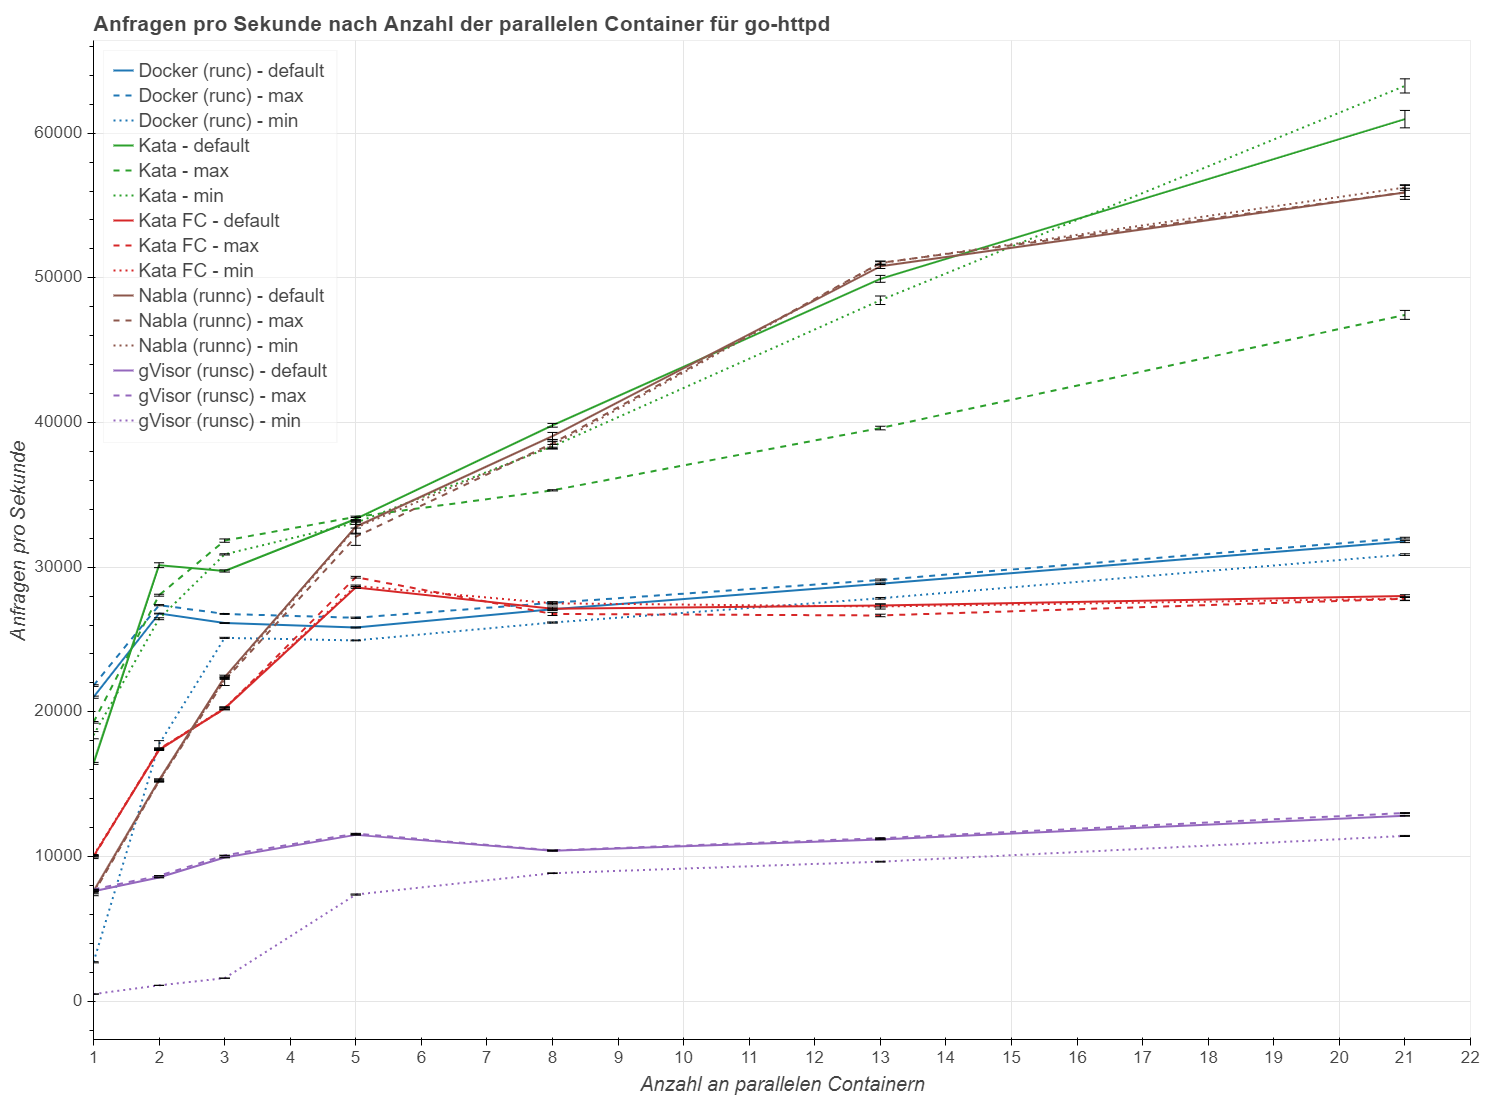
\includegraphics[width=0.98\linewidth]{gfx/auswertung/ab_go.png} 
		\label{fig:ab_go}}
		\caption{Anfragen pro Sekunde nach Skalierungsstufen}
	\end{figure}

	\begin{figure}[]
	\captionsetup{list=no}
	\ContinuedFloat 
	\centering 
	\subfloat[Anfragen pro Sekunde nach Skalierungsstufen für Httpd]
	{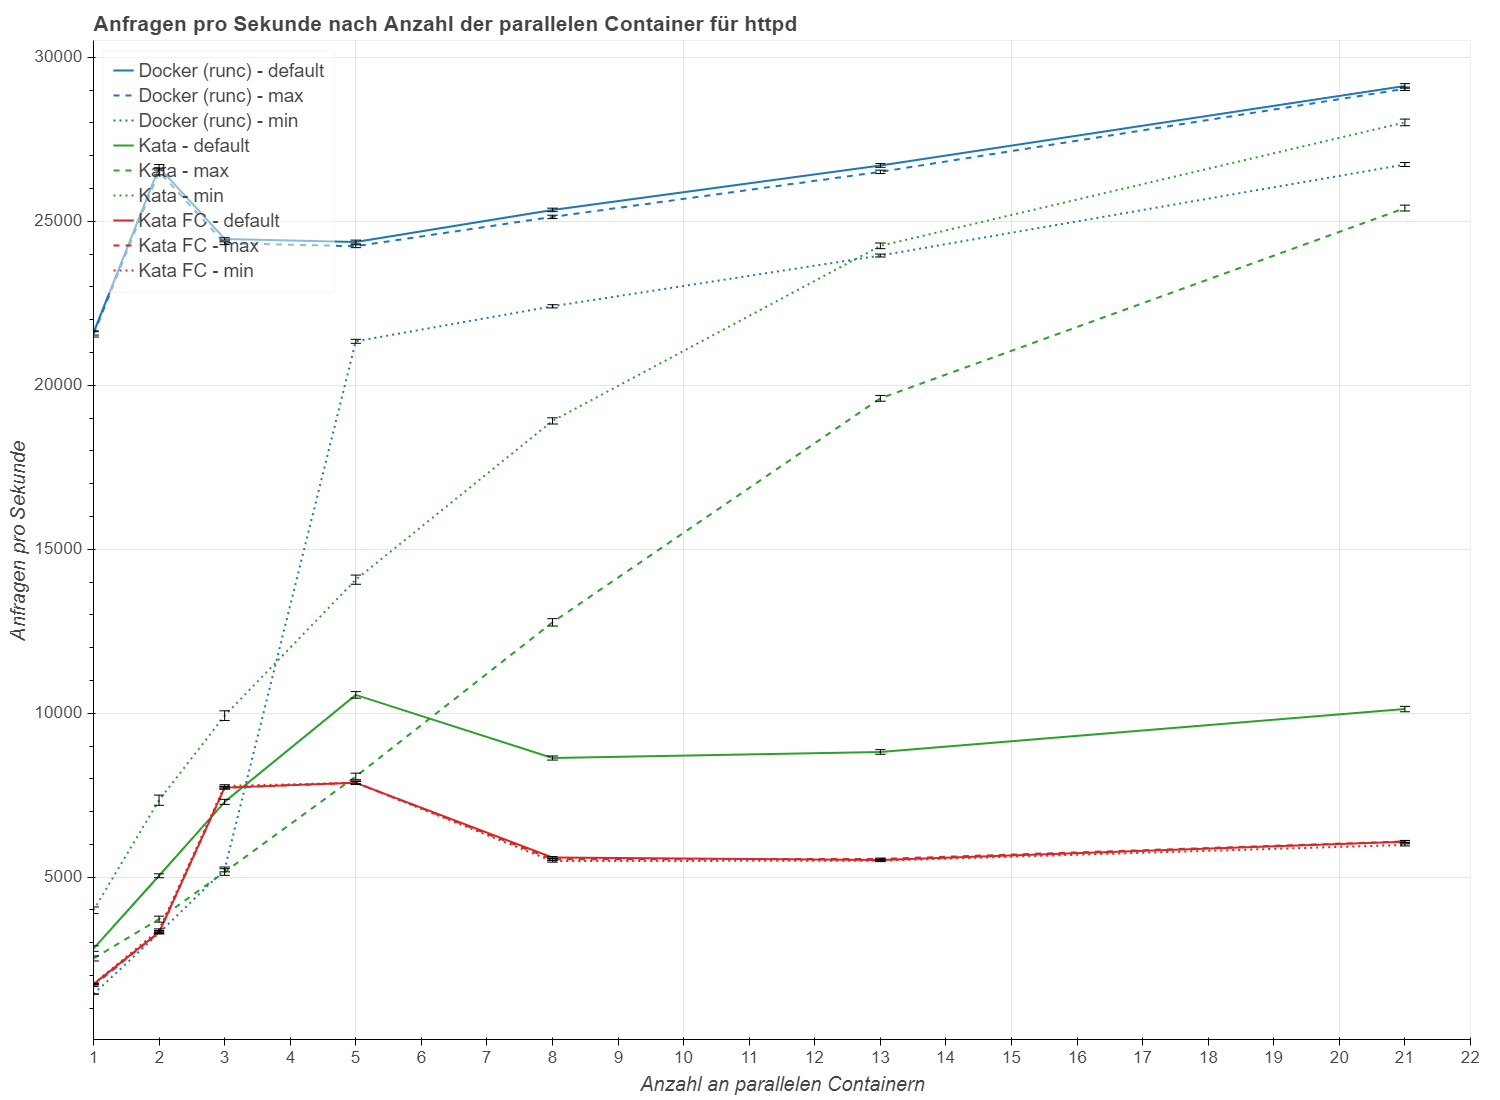
\includegraphics[width=0.98\linewidth]{gfx/auswertung/ab_httpd.png}
		\label{fig:ab_httpd}} \\
	\subfloat[Anfragen pro Sekunde nach Skalierungsstufen für Nginx]
	{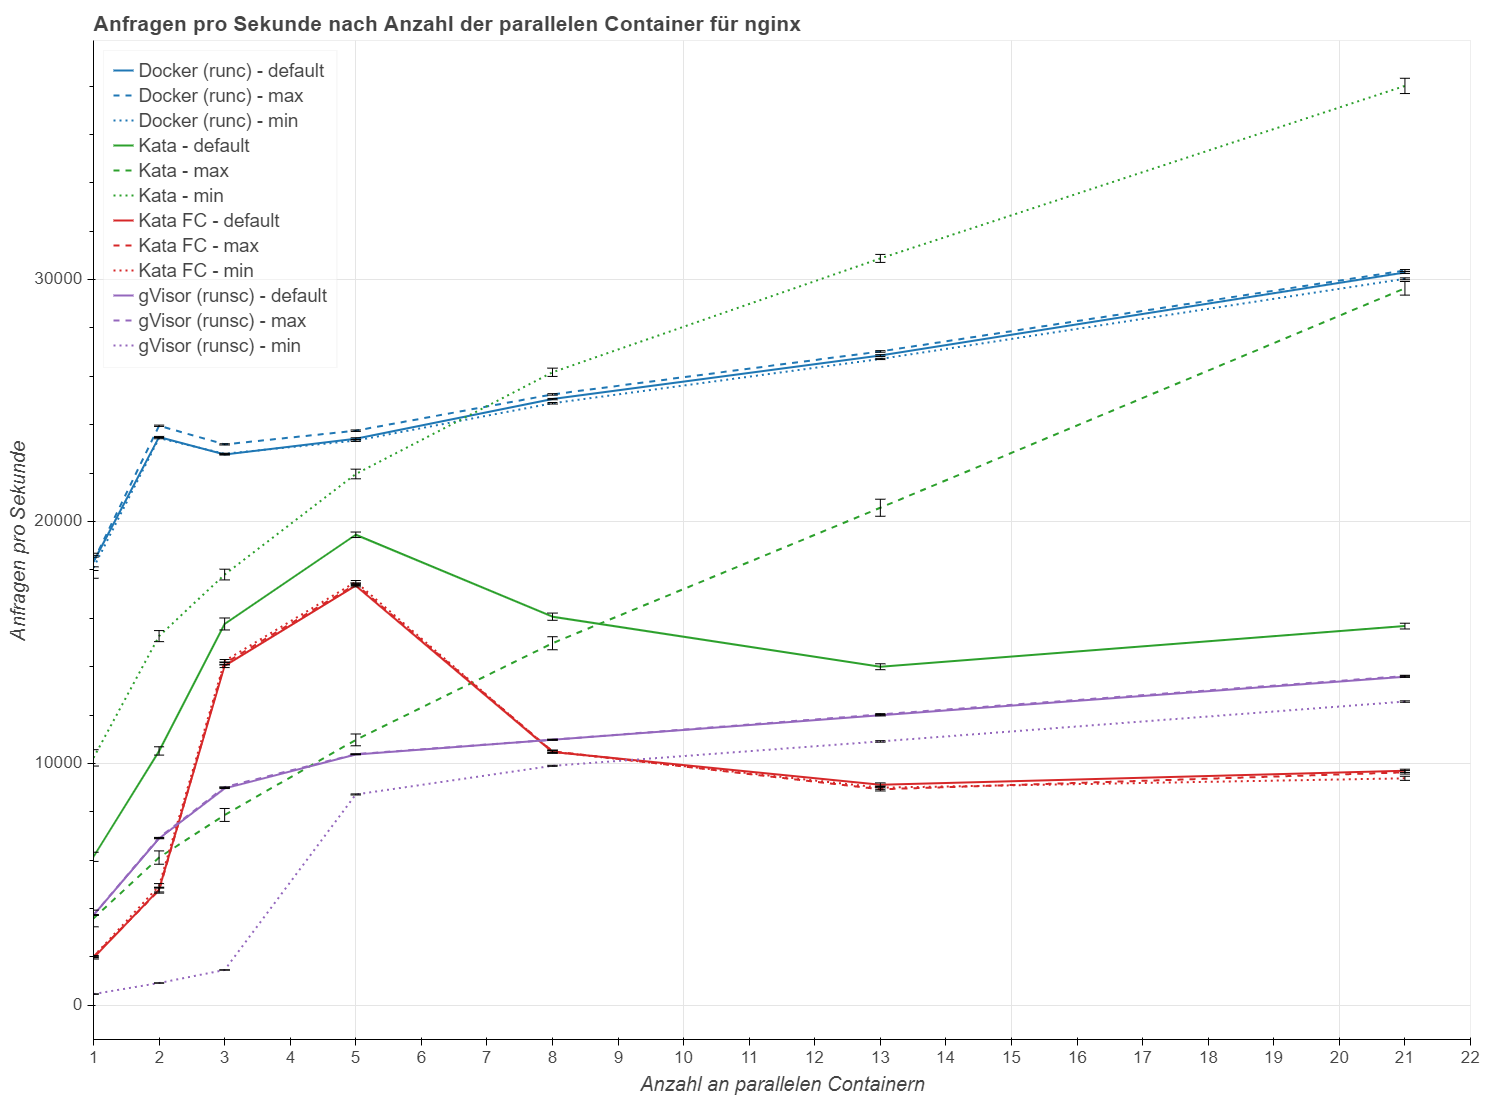
\includegraphics[width=0.98\linewidth]{gfx/auswertung/ab_nginx.png} 
		\label{fig:ab_nginx}}
	\caption{Anfragen pro Sekunde nach Skalierungsstufen}
\end{figure}

\begin{figure}[]
	\captionsetup{list=no}
	\ContinuedFloat 
	\centering 
	\subfloat[Anfragen pro Sekunde nach Skalierungsstufen für Python Tornado]
	{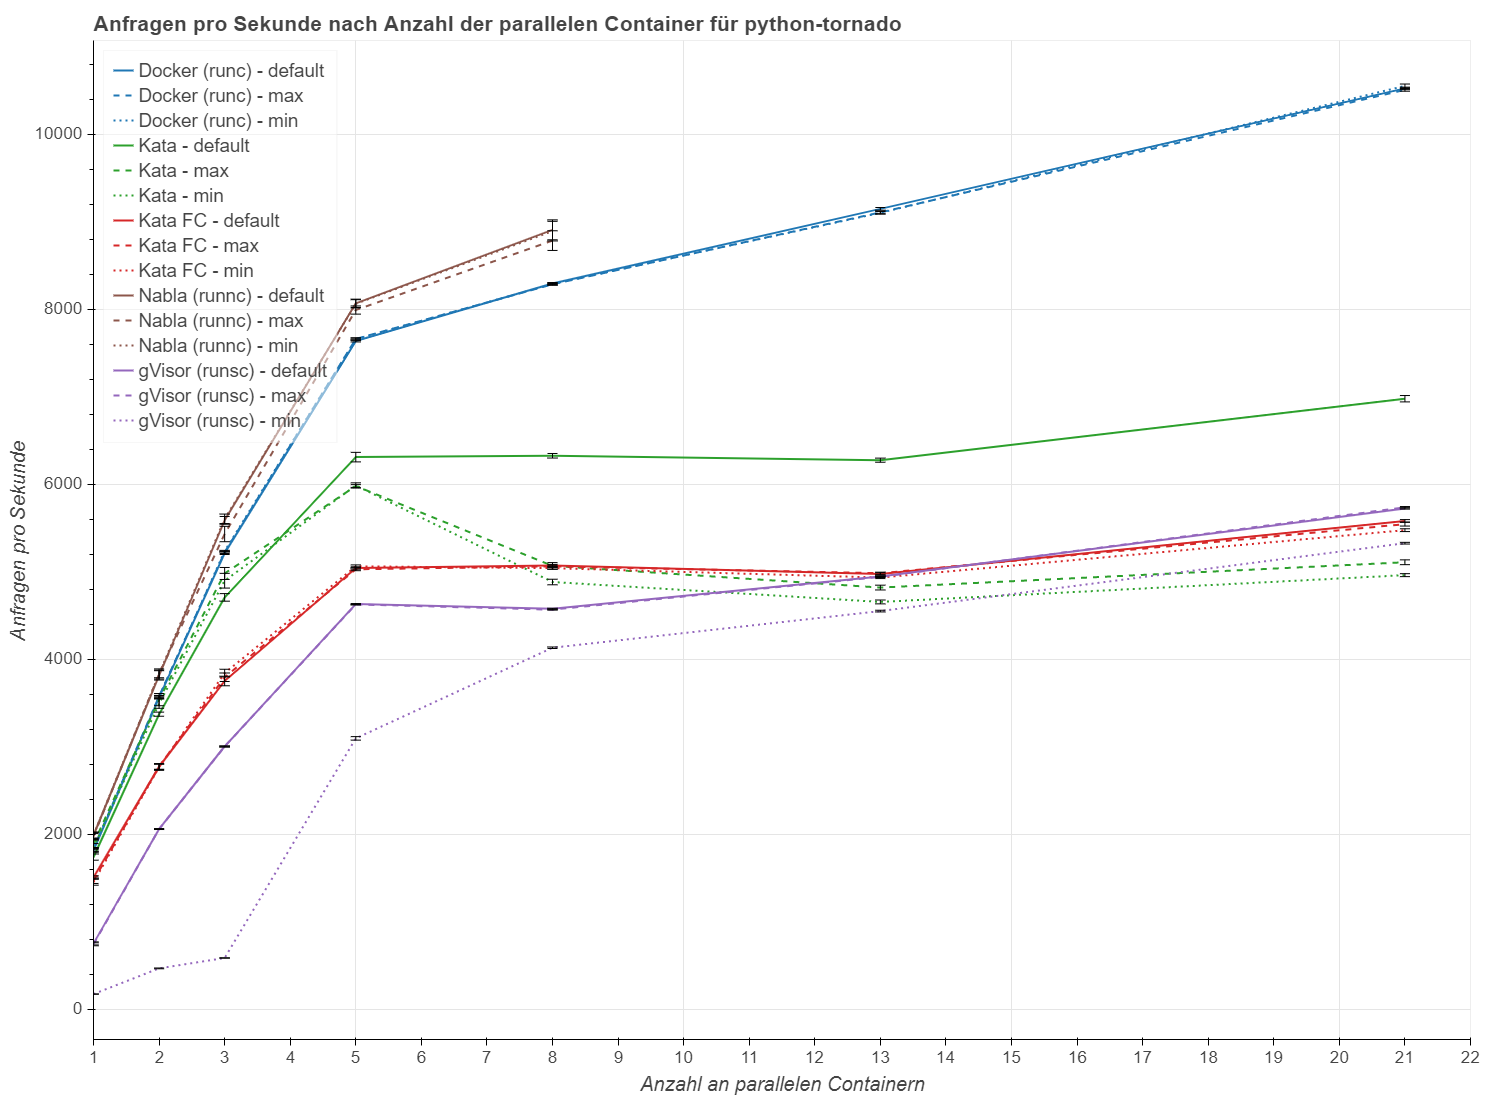
\includegraphics[width=0.98\linewidth]{gfx/auswertung/ab_python.png}
		\label{fig:ab_python}} \\
	\subfloat[Anfragen pro Sekunde nach Skalierungsstufen für Tomcat]
	{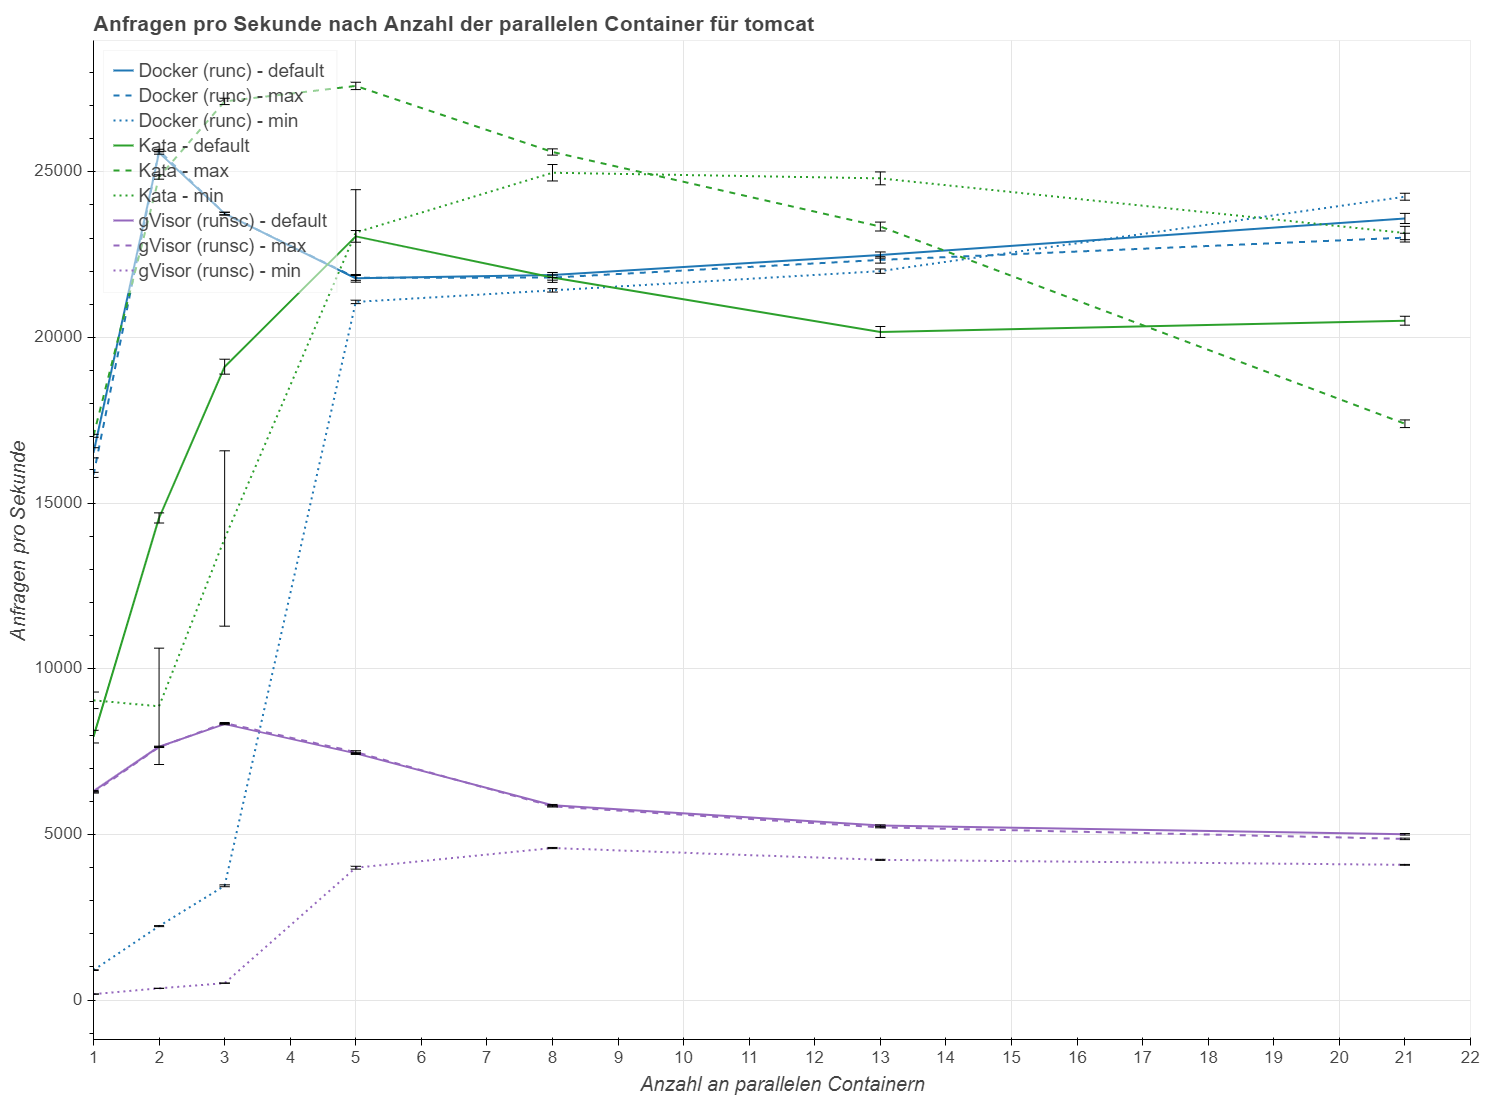
\includegraphics[width=0.98\linewidth]{gfx/auswertung/ab_tomcat.png} 
		\label{fig:ab_tomcat}}
	\caption{Anfragen pro Sekunde nach Skalierungsstufen}
\end{figure}


\subsection{Arbeitsspeicherverbrauch}
Während des ApacheBench Benchmarks wird der verwendete Arbeitsspeicher des Linux Systems gemessen. Die detaillierten Ergebnisse sind der Tabelle \ref{tbl:ramdetailauswertung} im Anhang zu entnehmen. Die Werte sind nach dem Skalierungsverhalten in den Graphen \ref{fig:ram_go}, \ref{fig:ram_httpd}, \ref{fig:ram_nginx}, \ref{fig:ram_python} und \ref{fig:ram_tomcat} visualisiert. Die Konfidenzintervalle sind in diesen Grafiken eingezeichnet.

Wenn kein statistisch signifikanter Unterschied zu Docker festzustellen ist, wird der Kandidat mit 100\% gewertet und in der Tabelle \ref{tbl:ramdetailauswertung} grau markiert.
Die Ergebnisse sind nach Image und Limits gruppiert und der Tabelle \ref{tbl:ramergebnis} zu entnehmen. Für die Images und die Limits wird der Schnitt gebildet. Weiter ist der Durchschnitt über alle Ergebnisse nach Kandidat angegeben. 

\begin{table}[h]
	\myfloatalign
	\small 
	\begin{tabularx}{\textwidth}{Xlrrrrr} \hline
		\spacedlowsmallcaps{Image} & \spacedlowsmallcaps{Limit} & \spacedlowsmallcaps{Docker} & \spacedlowsmallcaps{Kata} & \spacedlowsmallcaps{Kata FC} & \spacedlowsmallcaps{gVisor} & \spacedlowsmallcaps{Nabla} \\ \hline
		go-httpd & default & 100,00 & 157,12 & 87,88 & 304,29 & 93,70 \\
		go-httpd & min & 100,00 & 231,18 & 106,37 & 133,48 & 114,44 \\
		go-httpd & max & 100,00 & 407,58 & 105,11 & 164,06 & 119,50 \\ \hline
		\multicolumn{2}{l}{\textbf{Schnitt go-httpd}} & 100,00 & 265,29 & 99,75 & 200,61 & 109,20 \\ \hline
		httpd & default & 100,00 & 178,78 & 82,36 & - & - \\
		httpd & min & 100,00 & 219,09 & 83,64 & - & - \\
		httpd & max & 100,00 & 363,18 & 185,08 & - & - \\ \hline
		\multicolumn{2}{l}{\textbf{Schnitt httpd}} & 100,00 & 253,68 & 117,03 & - & - \\ \hline
		nginx & default & 100,00 & 145,12 & 96,61 & 123,78 & - \\
		nginx & min & 100,00 & 159,48 & 100,85 & 112,20 & - \\
		nginx & max & 100,00 & 238,15 & 112,98 & 112,97 & - \\ \hline
		\multicolumn{2}{l}{\textbf{Schnitt nginx}} & 100,00 & 180,92 & 103,48 & 116,32 & - \\ \hline
		python-tornado & default & 100,00 & 114,75 & 90,27 & 121,87 & 37,82 \\
		python-tornado & min & 100,00 & 139,81 & 93,49 & 104,21 & 41,02 \\
		python-tornado & max & 100,00 & 139,81 & 99,51 & 109,06 & 40,90\\ \hline
		\multicolumn{2}{l}{\textbf{Schnitt python-tornado}} & 100,00 & 131,46 & 94,42 & 111,71 & 39,91 \\ \hline
		tomcat & default & 100,00 & 126,76 & - & 59,45 & - \\
		tomcat & min & 100,00 & 160,05 & - & 28,04 & - \\
		tomcat & max & 100,00 & 175,58 & - & 34,69 & - \\ \hline
		\multicolumn{2}{l}{\textbf{Schnitt tomcat}} & 100,00 & 154,13 & - & 40,73 & - \\ \hline
		\textbf{Schnitt} & & 100,00 & 197,10 & 103,67 & 117,34 & 74,56 \\
		\hline
	\end{tabularx}
	\caption[Ergebnisse des Arbeitsspeicherverbrauchs Benchmarks]{Ergebnisse des Arbeitsspeicherverbrauchs Benchmarks}
	\footnotesize alle Angaben in Prozent, Werte kleiner 100 sind besser
	\label{tbl:ramergebnis}
\end{table}

Da mit der Messmethode das gesamte Linux System betrachtet wird, sind die Ergebnisse nicht exakt, daraus lassen sich aber Tendenzen ableiten.
Der Arbeitsspeicherverbrauch liegt bei Kata deutlich über Docker. In machen Fällen ist er drei oder viermal so hoch. Im Durchschnitt ist er doppelt so hoch wie der von Docker. Kata FC benötigt meist den gleichen Speicherplatz wie Docker. Nur im Fall von Nginx mit maximalen Limits belegt Kata FC 185\% des Speichers im Vergleich zu Docker. Der Verbrauch von gVisor bei den Images Nginx und Python Tornado liegt über dem von Docker. Im Betrieb von Go Httpd ist der Verbrauch doppelt so hoch, bei Tomcat weniger als halb so hoch. Nabla verwendet bei Go Httpd etwa gleich viel Arbeitsspeicher wie Docker, bei Python Tornado 40\%.

Insgesamt ist der Verbrauch von Kata fast doppelt so hoch wie der von Docker, was auf die Verwendung von Betriebssystemvirtualisierung zurückzuführen ist. Bei Kata FC ist die Arbeitsspeichernutzung mit Docker vergleichbar. Daraus lässt sich schließen, dass Firecracker weniger Arbeitsspeicher benötigt als Clear Linux und \ac{QEMU}.
gVisor liegt je nach Anwendungsfall über oder unter dem Verbrauch von Docker. Zusammenfassend ergibt sich ein Overhead von etwa 20\% im Speicherverbrauch. Beachtenswert ist, dass Nabla im Fall von Python Tornado deutlich unter dem Verbrauch von Docker liegt. 
Wird der Arbeitsspeicherverbrauch mit der Skalierung in Zusammenhang gebracht, wird ersichtlich, dass der Verbrauch mit steigender Skalierung zunimmt. Dabei ist die Steigung bei Kata am steilsten. Auffällig ist, dass sich für viele Runtimes der Tiefpunkt nicht bei einem, sondern bei zwei Containern befindet.
Die Kurven für die jeweiligen Limits liegen bei allen Runtimes dicht beieinander. Kata bildet die Ausnahme, bei dieser Runtime ist ein deutlicher Unterschied zwischen dem default und maximalen Limit ersichtlich.

\begin{figure}[h]
	\myfloatalign
	\subfloat[Arbeitsspeicherverbrauch nach Skalierungsstufen für Go Httpd]
	{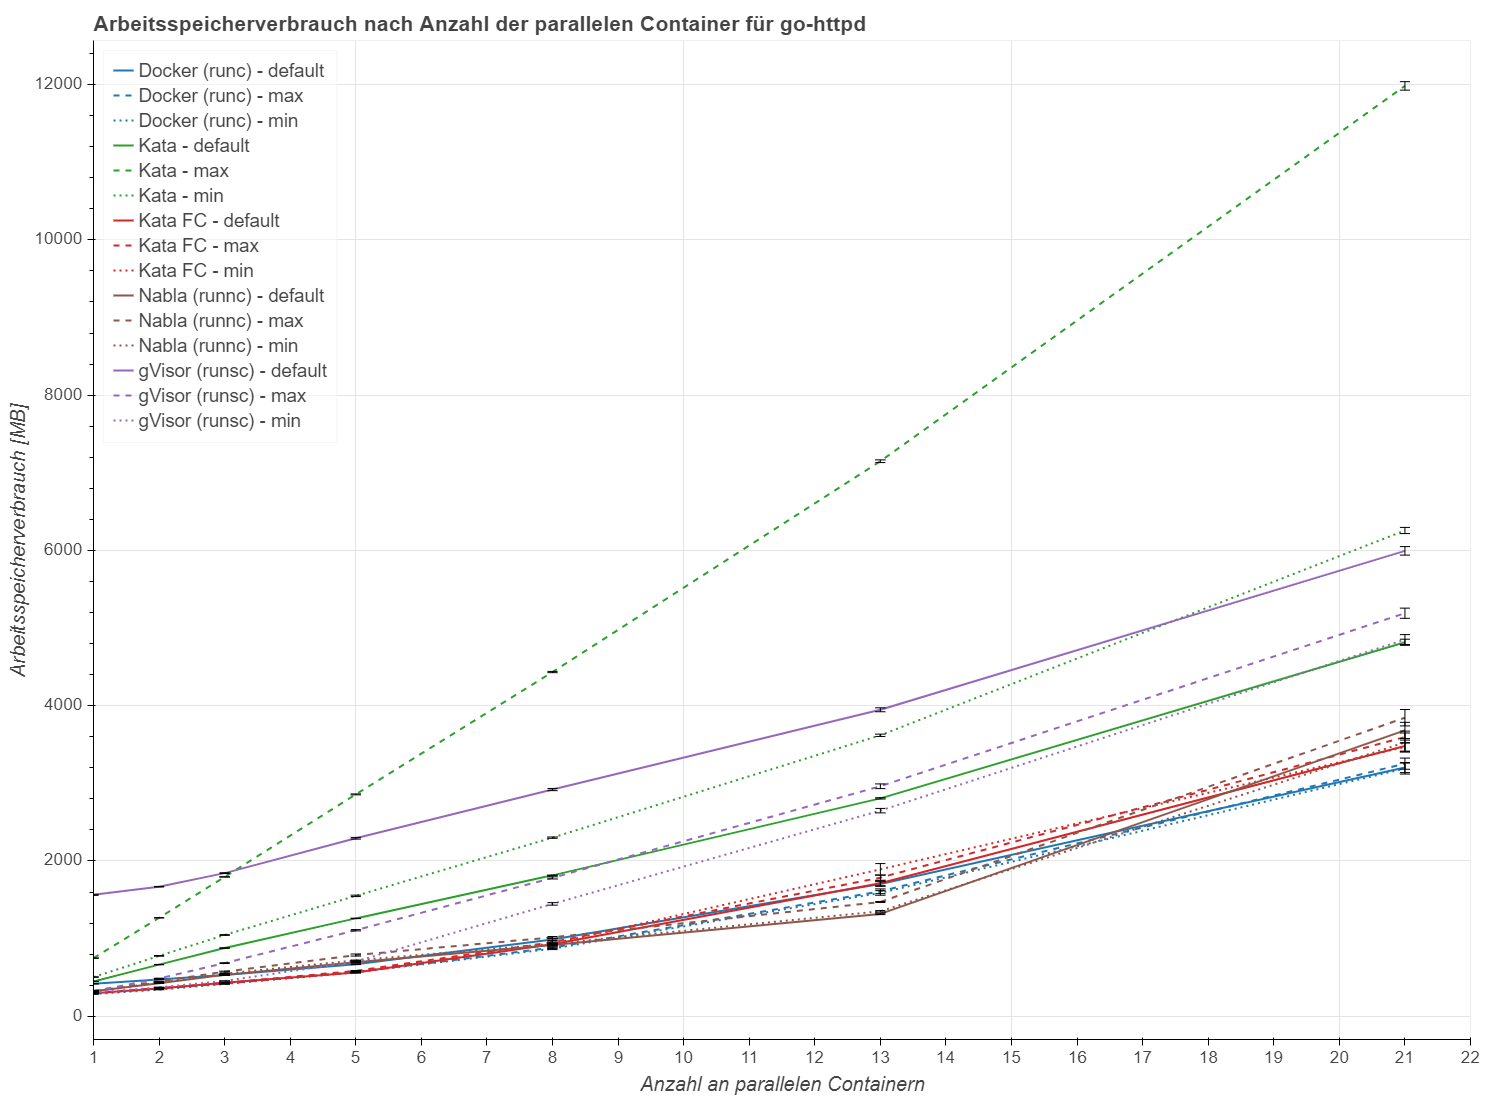
\includegraphics[width=0.98\linewidth]{gfx/auswertung/ram_go.png} 
		\label{fig:ram_go}} 
	\caption{Arbeitsspeicherverbrauch nach Skalierungsstufen}
\end{figure}

\begin{figure}[]
	\ContinuedFloat 
	\captionsetup{list=no}
	\centering 
	\subfloat[Arbeitsspeicherverbrauch nach Skalierungsstufen für Httpd]
	{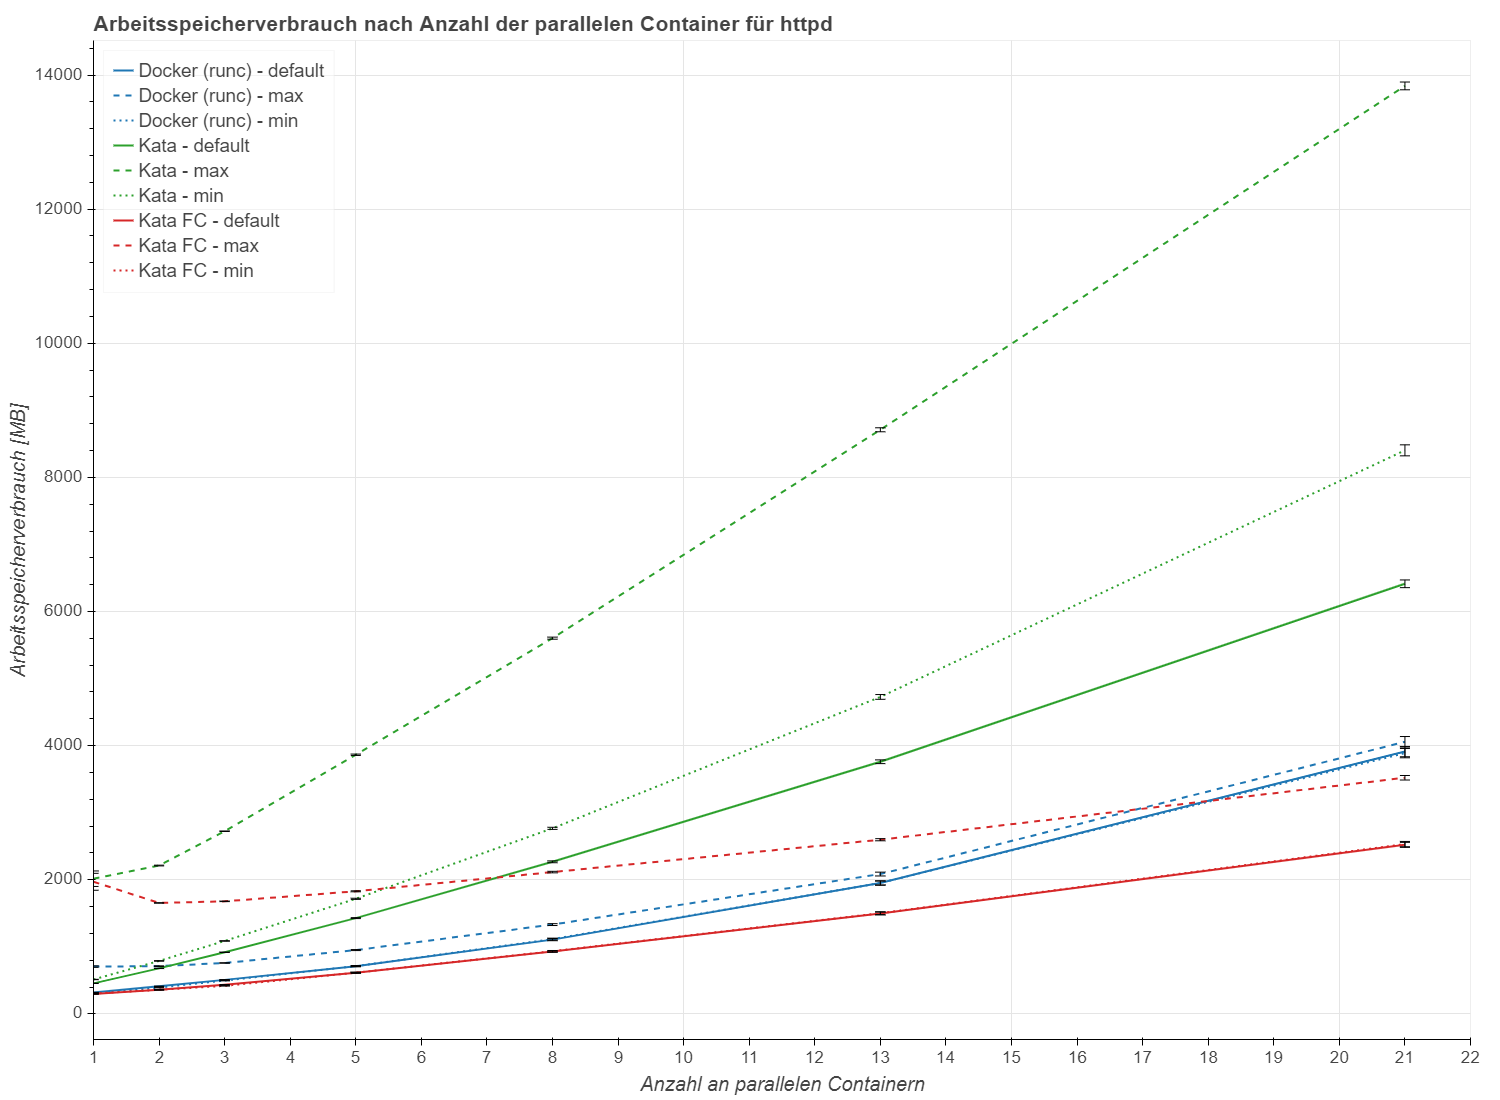
\includegraphics[width=0.98\linewidth]{gfx/auswertung/ram_httpd.png}
		\label{fig:ram_httpd}} \\
	\subfloat[Arbeitsspeicherverbrauch nach Skalierungsstufen für Nginx]
	{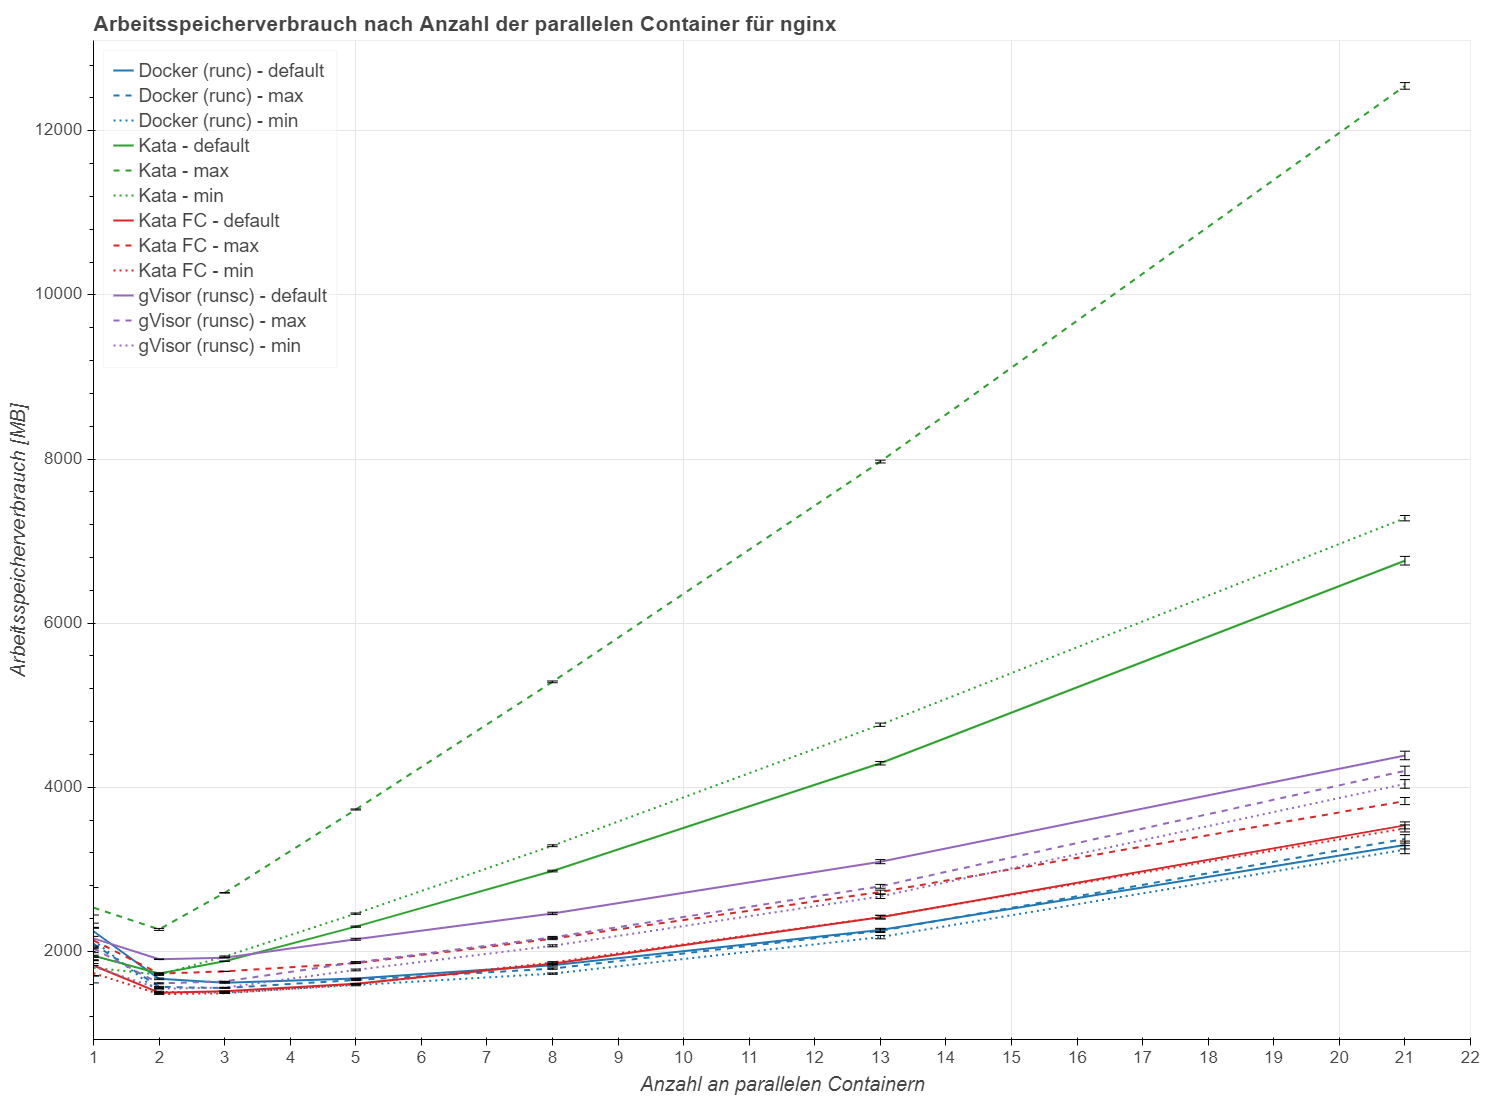
\includegraphics[width=0.98\linewidth]{gfx/auswertung/ram_nginx.png} 
		\label{fig:ram_nginx}} \\
	\caption{Arbeitsspeicherverbrauch nach Skalierungsstufen}
\end{figure}

\begin{figure}[]
	\ContinuedFloat 
	\centering 
	\captionsetup{list=no}
	\subfloat[Arbeitsspeicherverbrauch nach Skalierungsstufen für Python Tornado]
	{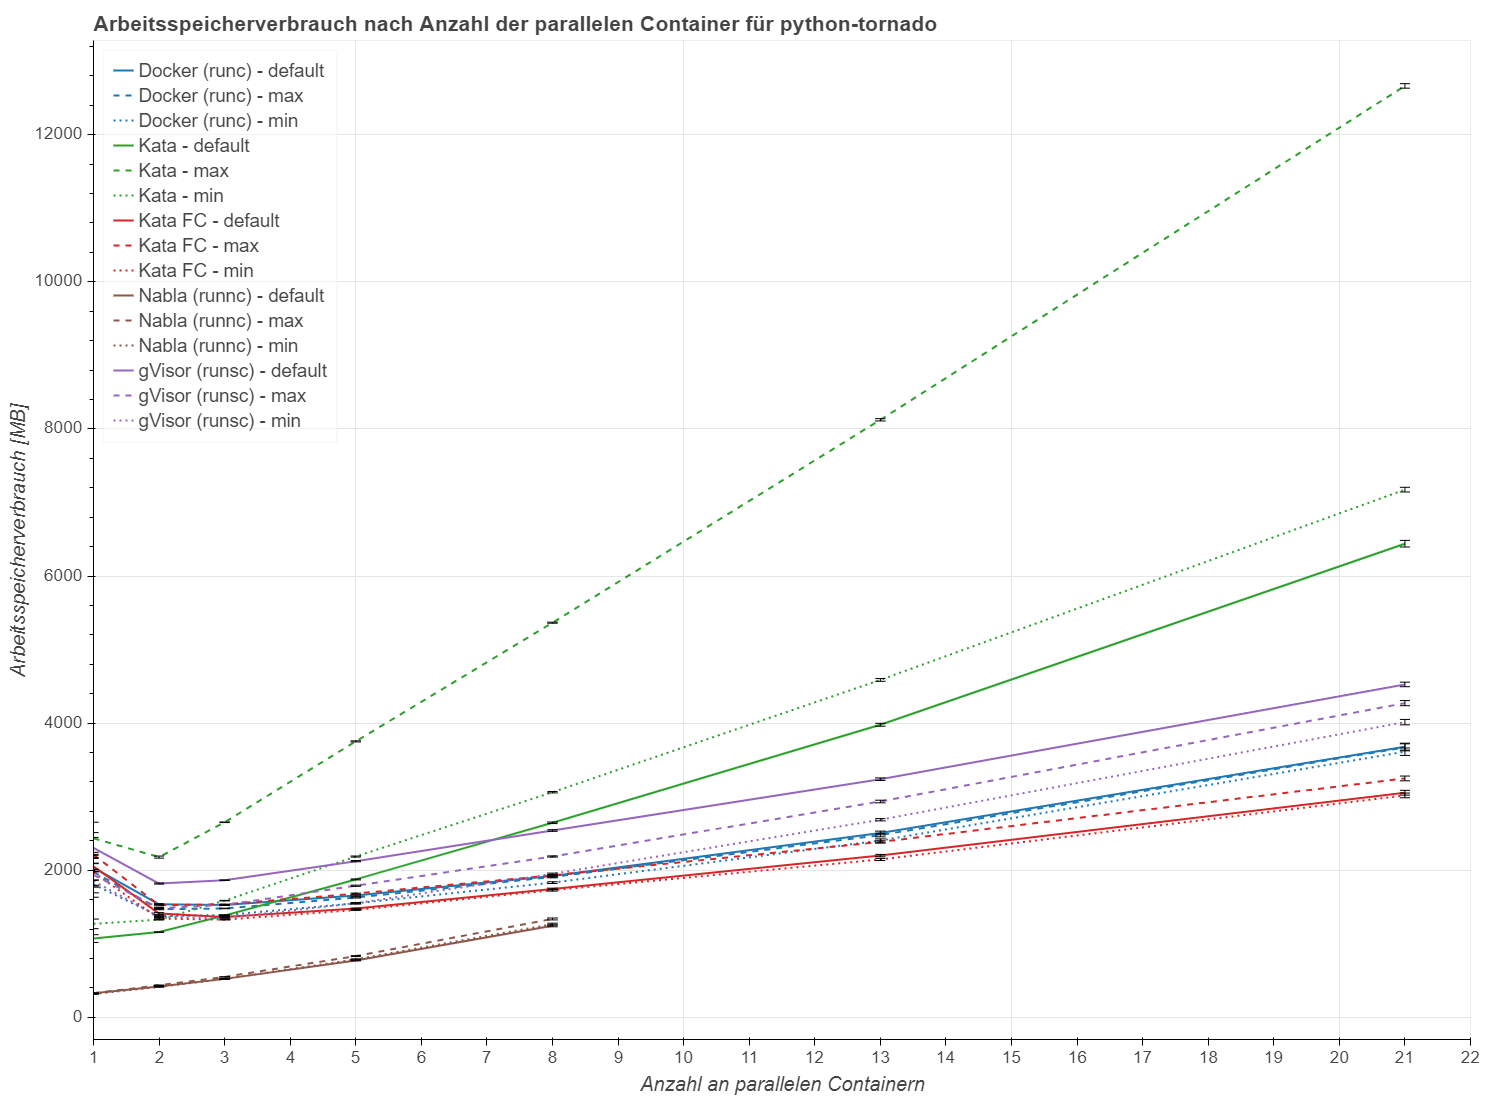
\includegraphics[width=0.98\linewidth]{gfx/auswertung/ram_python.png}
		\label{fig:ram_python}} \\
	\subfloat[Arbeitsspeicherverbrauch nach Skalierungsstufen für Tomcat]
	{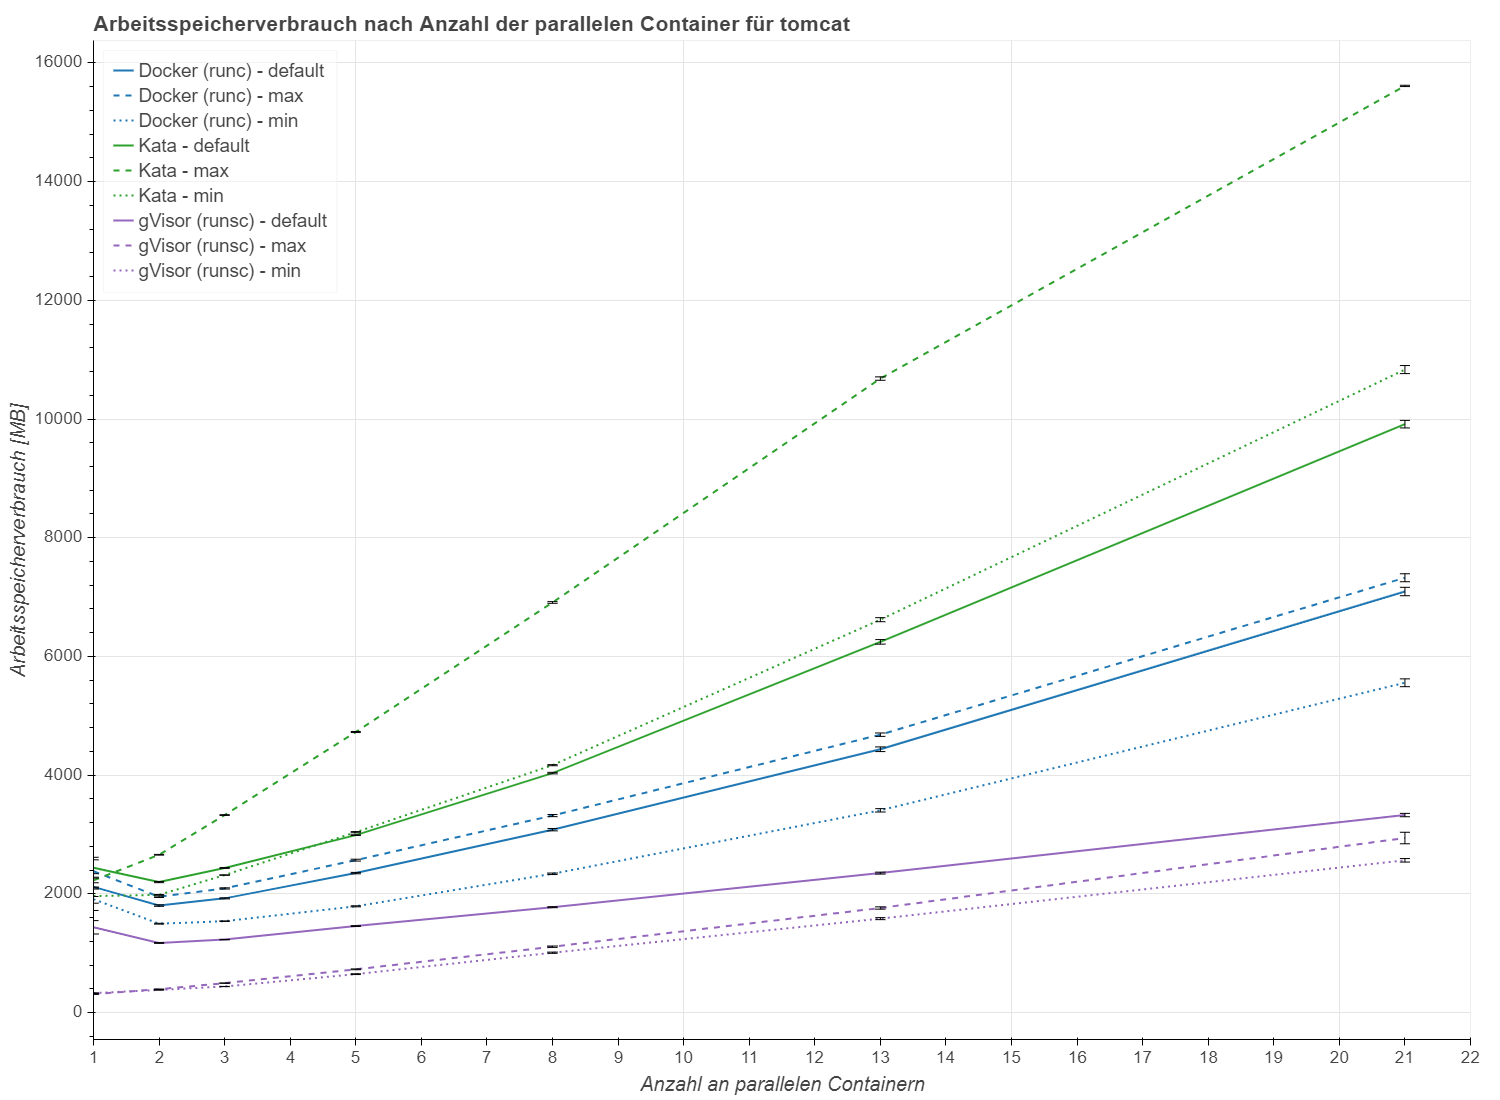
\includegraphics[width=0.98\linewidth]{gfx/auswertung/ram_tomcat.png} 
		\label{fig:ram_tomcat}}
	\caption{Arbeitsspeicherverbrauch nach Skalierungsstufen}
\end{figure}

\subsection{Dauer des Startens und Entfernens eines Containers}
Die Dauer der Containererzeugung und -entfernung wird mit dem Bash Programm time gemessen. Alle Fälle, in denen kein statistisch signifikanter Unterschied festzustellen ist, werden in den Tabellen \ref{tbl:timeuperfergebnis} und \ref{tbl:timermerfergebnis} im Anhang grau markiert und mit 100\% gewertet. Die Messergebnisse werden nach Image und Limits gruppiert und sind im Anhang den Tabellen \ref{tbl:timeuperfergebnis} für die Dauer des Startens und \ref{tbl:timermerfergebnis} für die Dauer des Entfernens zu entnehmen. Für die einzelnen Images und über alle Kandidaten wird der Durchschnitt gebildet. Für einen Überblick werden die Ergebnisse nach den Images gruppiert und sind Tabelle \ref{tbl:timeup} für die Dauer des Startens und Tabelle \ref{tbl:timerm} für die Dauer des Entfernens zu entnehmen.

\begin{table}[h]
	\myfloatalign
	\small 
	\begin{tabularx}{\textwidth}{Xrrrrr} \hline
		\spacedlowsmallcaps{Image} & \spacedlowsmallcaps{Docker} & \spacedlowsmallcaps{Kata} & \spacedlowsmallcaps{Kata FC} & \spacedlowsmallcaps{gVisor} & \spacedlowsmallcaps{Nabla} \\ \hline
		alpine        & 100,00 & 193,16 & 334,12  & 105,58 & -      \\
		busybox       & 100,00 & 192,29 & 326,89  & 103,38 & -      \\
		go-httpd      & 100,00 & 177,94 & 310,51  & 103,23 & 340,61 \\
		httpd         & 100,00 & 178,49 & 310,06  & 103,24 & -      \\
		mongo         & 100,00 & 179,48 & 306,90  & 106,42 & -      \\
		nginx         & 100,00 & 180,42 & 313,42  & 105,02 & -      \\
		node-express  & 100,00 & 182,36 & 315,07  & 104,60 & 345,77 \\
		postgres      & 100,00 & 179,24 & 308,22  & 107,04 & -      \\
		python-tornado& 100,00 & 179,96 & 312,69  & 103,65 & 135,31 \\
		redis-test    & 100,00 & 179,59 & 312,32  & 105,69 & 117,11 \\
		tomcat        & 100,00 & 180,08 & 312,87  & 106,27 & -      \\
		traefik       & 100,00 & 179,73 & 314,65  & 105,30 & -      \\
		ubuntu        & 100,00 & 196,58 & 334,35  & 105,41 & -      \\ \hline
		\textbf{Schnitt}   & 100,00 & 183,02 & 316,31  & 104,99 & 234,70 \\
		\hline
	\end{tabularx}
	\caption[Dauer des Startens eines Containers]{Dauer des Startens eines Containers nach den Images}
	\footnotesize alle Angaben in Prozent, Werte kleiner 100 sind besser
	\label{tbl:timeup}
\end{table}

Beim Starten eines Containers sind über alle Images hinweg klare Tendenzen sichtbar. Kata FC benötigt über die dreifache Zeit zum Starten verglichen mit Docker. GVisor ist nur wenig langsamer als Docker und bei Kata dauert der Start 180\% der Zeit von Docker. Bei Nabla liegen die Startzeiten bei den Images Go Httpd und Node Express mit ca. 340\% deutlich über den Werten und bei den Images Python Tornado und Redis mit 135\% und 117\% nur geringfügig über den Werten von Docker.

Bei der Untersuchung zur Dauer für das Entfernen eines Containers liegen die Werte näher beieinander. Kata ist mit 141\% und Kata FC mit 172\% langsamer als Docker. Die Zeiten von gVisor sind mit denen von Docker vergleichbar. Einzig Nabla ist beim Entfernen mit 62\% schneller als Docker.

Werden die Ergebnisse nach den Ressourcenlimits gruppiert, vgl. Tabelle \ref{tbl:timenachlimits}, wird deutlich, dass sich die Werte zwischen den Limits sowohl beim Starten, als auch beim Entfernen kaum unterscheiden. Einzig die Startzeiten bei Kata mit einem maximalen Ressourcenlimit sind deutlich über den Zeiten mit einem default Limit. 

\begin{table}[h]
	\small 
	\myfloatalign
	\begin{tabularx}{\textwidth}{Xrrrrr} \hline
		\spacedlowsmallcaps{Image} & \spacedlowsmallcaps{Docker} & \spacedlowsmallcaps{Kata} & \spacedlowsmallcaps{Kata FC} & \spacedlowsmallcaps{gVisor} & \spacedlowsmallcaps{Nabla} \\ \hline
		alpine        & 100,00 & 143,07 & 152,86  & 100,00 & -     \\
		busybox       & 100,00 & 145,56 & 159,10  & 100,00 & -     \\
		go-httpd      & 100,00 & 129,34 & 155,33  & 105,87 & 74,94 \\
		httpd         & 100,00 & 142,16 & 177,88  & 109,32 & -     \\
		mongo         & 100,00 & 148,24 & 198,84  & 110,67 & -     \\
		nginx         & 100,00 & 136,91 & 172,27  & 109,85 & -     \\
		node-express  & 100,00 & 134,91 & 171,84  & 107,98 & 72,03 \\
		postgres      & 100,00 & 142,36 & 214,06  & 106,54 & -     \\
		python-tornado& 100,00 & 148,22 & 154,91  & 76,26  & 48,43 \\
		redis-test    & 100,00 & 135,66 & 162,57  & 111,12 & 53,14 \\
		tomcat        & 100,00 & 135,04 & 173,71  & 107,00 & -     \\
		traefik       & 100,00 & 142,17 & 184,19  & 111,32 & -     \\
		ubuntu        & 100,00 & 143,48 & 154,68  & 108,34 & -     \\ \hline
		\textbf{Schnitt}                & 100,00 & 140,55 & 171,71  & 104,94 & 62,14\\
		\hline
	\end{tabularx}
	\caption[Dauer des Entfernens eines Containers]{Dauer des Entfernens eines Containers nach den Images}
	\footnotesize alle Angaben in Prozent, Werte kleiner 100 sind besser
	\label{tbl:timerm}
\end{table}


\begin{table}[h]
	\small 
	\myfloatalign
	\begin{tabularx}{\textwidth}{Xlrrrrr} \hline
		\spacedlowsmallcaps{Messung} & \spacedlowsmallcaps{Limit} & \spacedlowsmallcaps{Docker} & \spacedlowsmallcaps{Kata} & \spacedlowsmallcaps{Kata FC} & \spacedlowsmallcaps{gVisor} & \spacedlowsmallcaps{Nabla} \\ \hline
		Starten   & default & 100,00    & 162,82 & 319,14  & 104,53 & 236,49 \\
		Starten   & min     & 100,00    & 170,99 & 314,01  & 105,41 & 236,49 \\
		Starten   & max     & 100,00    & 215,27 & 315,79  & 105,02 & 231,13 \\ \hline
		Entfernen & default & 100,00    & 139,27 & 167,83  & 105,43 & 67,62  \\
		Entfernen & min     & 100,00    & 142,67 & 175,51  & 104,93 & 57,26  \\
		Entfernen & max     & 100,00    & 139,7  & 171,79  & 104,48 & 61,53  \\ 
		\hline
	\end{tabularx}
	\caption[Dauer des Startens und Entfernens nach Limits]{Dauer des Startens und Entfernens eines Containers nach Limits}
	\footnotesize alle Angaben in Prozent, Werte kleiner 100 sind besser
	\label{tbl:timenachlimits}
\end{table}

\subsection{Netzwerkbandbreite}
Mithilfe der Software iPerf wird die Netzwerkbandbreite für das Senden und Empfangen von Daten mit den Protokollen \ac{TCP} und \ac{UDP} gemessen. Die Messung wird ohne Nabla als Kandidat durchgeführt. Bei den Messungen mit dem Protokoll \ac{TCP} sind immer statistisch signifikante Unterschiede festzustellen. Bei allen \ac{UDP} Messungen ist die Messgenauigkeit nicht ausreichend, um einen Unterschied zu identifizieren. Daher werden diese Fälle mit 100\% gewertet. Die Ergebnisse werden nach Limits gruppiert und sind der Tabelle \ref{tbl:iperfergebnis} zu entnehmen. Für die Limits wird ein Schnitt gebildet. Zusätzlich wird der Durchschnitt über alle Ergebnisse nach Kandidat angegeben.

Die Abweichungen von Kata und Kata FC zu Docker sind bei \ac{TCP} und \ac{UDP} sehr gering. Auch bei gVisor ist bei den Limits default und maximal und dem Protokoll \ac{TCP} kein Unterschied zu Docker zu erkennen. Auffällig ist, dass bei minimalen Limits und dem Protokoll \ac{TCP} die Leistung von gVisor bei 37\% von Docker liegt. Für das Protokoll \ac{UDP} liegen keine Messergebnisse für gVisor vor. 

In der Dokumentation von gVisor wird auch die Netzwerkbandbreite mit iPerf untersucht. Verglichen werden hier Docker und gVisor. Dabei liegt gVisor hinter Docker, die verwendeten Ressourcenlimits sind dabei nicht angegeben \cite[vgl.][]{gVisor.20200122b}. Abgesehen von den Messungen mit minimalem Limit, stimmt diese Untersuchung mit der eigenen überein.

\begin{table}[h]
	\myfloatalign
	\small 
	\begin{tabularx}{\textwidth}{Xlrrrr} \hline
		\spacedlowsmallcaps{Messung} & \spacedlowsmallcaps{Limit} & \spacedlowsmallcaps{Docker} & \spacedlowsmallcaps{Kata} & \spacedlowsmallcaps{Kata FC} & \spacedlowsmallcaps{gVisor} \\ \hline
		Senden TCP & default & 100,00 & 99,88 & 99,29 & 99,90 \\
		Senden TCP & min & 100,00 & 99,92 & 99,45 & 37,25 \\
		Senden TCP & max & 100,00 & 99,88 & 99,43 & 99,87 \\ \hline
		\multicolumn{2}{l}{\textbf{Schnitt Senden TCP}} & 100,00 & 99,89 & 99,39 & 79,01 \\ \hline
		Empfangen TCP & default & 100,00 & 99,84 & 99,20 & 99,90 \\
		Empfangen TCP & min & 100,00 & 99,88 & 99,35 & 37,06 \\
		Empfangen TCP & max & 100,00 & 99,85 & 99,35 & 99,89 \\ \hline
		\multicolumn{2}{l}{\textbf{Schnitt Empfangen TCP}} & 100,00 & 99,86 & 99,30 & 78,95 \\ \hline
		Senden UDP & default & 100,00 & 100,00 & 100,00 & - \\
		Senden UDP & min & 100,00 & 100,00 & 100,00 & - \\
		Senden UDP & max & 100,00 & 100,00 & 100,00 & - \\ \hline
		\multicolumn{2}{l}{\textbf{Schnitt Senden UDP}} & 100,00 & 100,00 & 100,00 & - \\ \hline
		\textbf{\textbf{Schnitt}} & & 100,00 & 99,92 & 99,56 & 78,98 \\ 	\hline
	\end{tabularx}
	\caption[Ergebnisse des iPerf Benchmarks]{Ergebnisse des iPerf Benchmarks}
	\footnotesize alle Angaben in Prozent, Werte größer 100 sind besser
	\label{tbl:iperfergebnis}
\end{table}

\subsection{Prozessorleistung}
Mithilfe der Software Linpack wird die Rechenleistung des Prozessors in Gleitkommaoperationen pro Sekunde gemessen. Die Messung wird ohne gVisor und Nabla als Kandidaten durchgeführt. Bei den Messungen sind immer statistisch signifikante Unterschiede festzustellen. Die Ergebnisse werden nach Limits gruppiert und sind Tabelle \ref{tbl:linpackergebnis} zu entnehmen. Weiter ist der Durchschnitt über alle Werte nach Kandidat angegeben. Die Ergebnisse sind in Abbildung \ref{fig:linpackergebnisse} dargestellt.

\begin{table}[h]
	\small 
	\myfloatalign 
	\begin{tabularx}{\textwidth}{Xrrr} \hline
		\spacedlowsmallcaps{Limit} & \spacedlowsmallcaps{Docker} & \spacedlowsmallcaps{Kata} & \spacedlowsmallcaps{Kata FC} \\ \hline
		default & 100,00 & 25,95 & 25,61 \\
		min & 100,00 & 343,06 & 427,76 \\
		max & 100,00 & 98,32 & 25,60 \\ \hline
		\textbf{Schnitt} & 100,00 & 155,78 & 159,66 \\\hline
	\end{tabularx}
	\caption[Ergebnisse des Linpack Benchmarks]{Ergebnisse des Linpack Benchmarks}
	\footnotesize alle Angaben in Prozent, Werte größer 100 sind besser
	\label{tbl:linpackergebnis}
\end{table}

Wird das maximale Ressourcenlimit betrachtet, kann Kata die Leistung von Docker annähernd erreichen. Kata FC dagegen erreicht nur ein Viertel der Rechenleistung. Bei der default Limitierung berechnen Kata und Kata FC nur ein Viertel der Gleitkommaoperationen pro Sekunden im Vergleich zu Docker. Dies lässt darauf schließen, dass ein Docker Container bei diesem Limit alle CPUs verwenden kann und Kata nicht. Beachtenswert ist, dass Kata und Kata FC bei minimalem Ressourcenlimits über die drei- oder vierfache Rechenleistung von Docker verfügen.

\begin{figure}[h]
	\myfloatalign
	\subfloat[Default Limit]
	{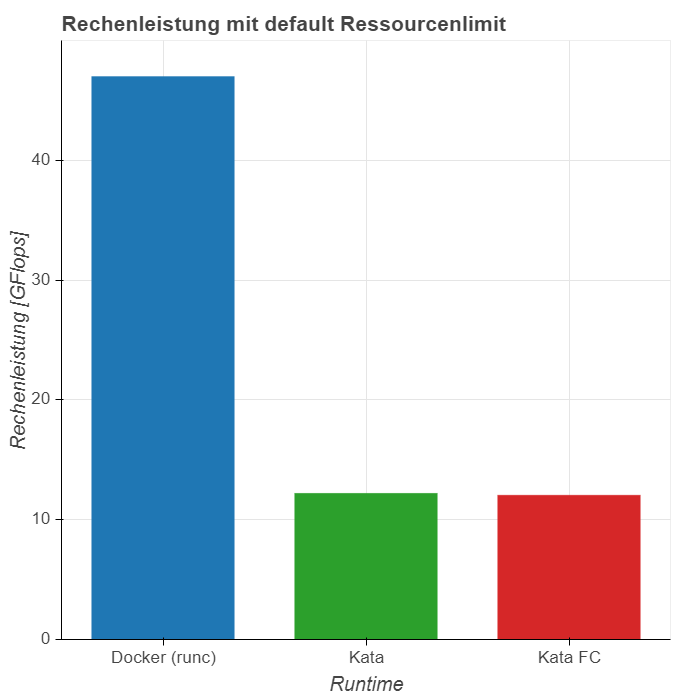
\includegraphics[width=.48\linewidth]{gfx/auswertung/linpack_default.png}} \quad
	\subfloat[Minimales Limit]
	{\label{fig:example-b}%
	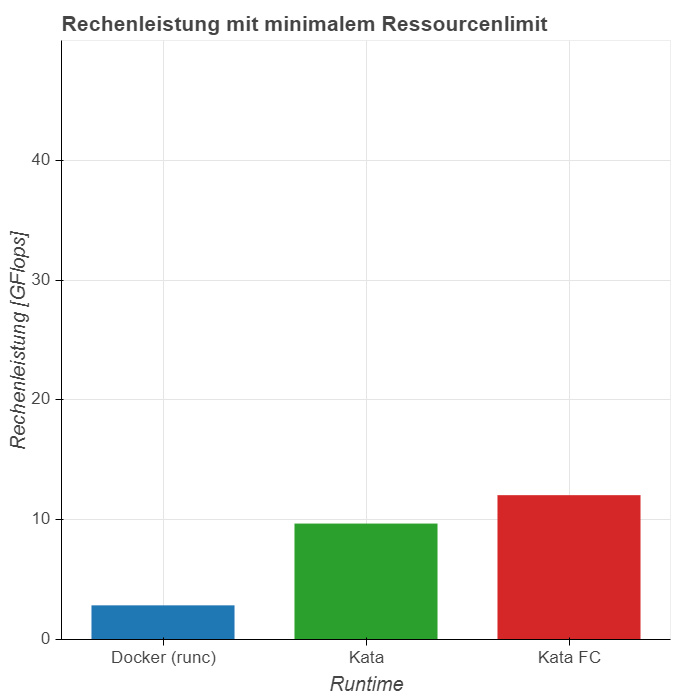
\includegraphics[width=.48\linewidth]{gfx/auswertung/linpack_min.png}} \\
	\subfloat[Maximales Limit]
	{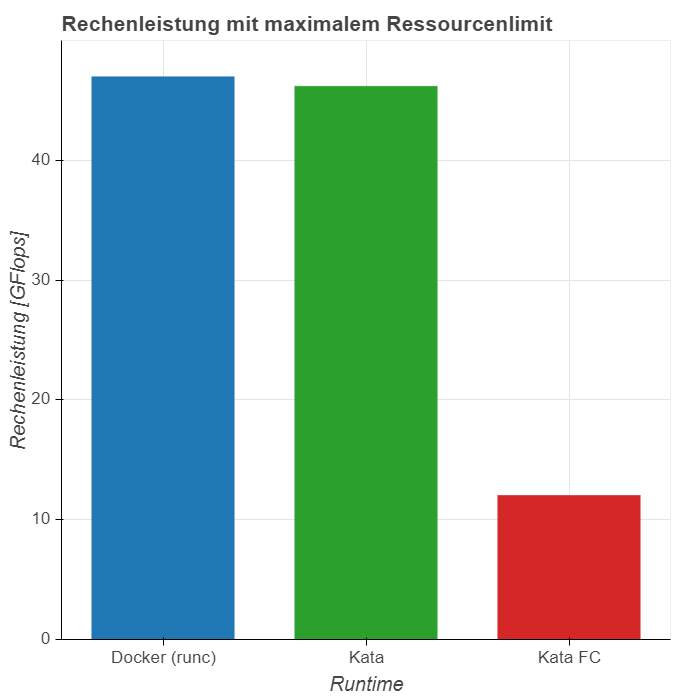
\includegraphics[width=.48\linewidth]{gfx/auswertung/linpack_max.png}} \quad
	\caption[Ergebnisse des Linpack Benchmarks]{Ergebnisse des Linpack Benchmarks nach Ressourcenlimits}
	\label{fig:linpackergebnisse}
\end{figure}

\newpage

\section{Einhaltung von Ressourcenlimits}
\label{sec:resslimits}
Die Untersuchungen zur Leistungsfähigkeit werden dazu verwendet um festzustellen, ob die gesetzten Ressourcenlimits Anwendung finden. Dieses Ergebnis wird für die Bewertung in Abschnitt \ref{sec:auswertung_dos} benötigt. Für die Runtimes Nabla und Kata FC ist nicht vollständig dokumentiert, inwieweit die Ressourcenlimits angewendet werden. 

Werden die Graphen zum Arbeitsspeicherverbrauch betrachtet, wird ersichtlich, dass Nabla bei jedem Ressourcenlimit den gleichen Verbrauch hat. Aus diesem Grund wird davon ausgegangen, dass Nabla keine Limitierung des Arbeitsspeichers vornimmt, vgl. Abbildung \ref{fig:ram_go} und \ref{fig:ram_python}. Bei der Untersuchung zur Webserverleistung unterscheidet sich die Leistung von Nabla bei den einzelnen Limits nicht. Nabla wendet hier keine Ressourcenlimitierung an.
In den Graphen zum Arbeitsspeicherverbrauch verläuft die Kurve von Kata FC mit maximalem Limit meist über der von default und minimalem Limit, vgl. Abbildung \ref{fig:ram_httpd}, \ref{fig:ram_nginx} und \ref{fig:ram_python}. Beim Betrieb des Images Go Httpd ist dieser Abstand kaum festzustellen, vgl. Abbildung \ref{fig:ram_go}. Die Limitierung des Arbeitsspeichers scheint also Auswirkungen auf den Verbrauch zu haben. Dabei ist anzunehmen, dass die Limitierung auf \ac{VM} Ebene und nicht für den Container in der \ac{VM} erfolgt. 

Zur Untersuchung der Rechenleistung mithilfe des Linpack Benchmarks werden die Ergebnisse dieses Benchmarks nicht gewichtet und in GFlops angegeben. Die Werte sind Tabelle \ref{tbl:linpackergebnisingflops} zu entnehmen. Dabei wird ersichtlich, dass sich die Ergebnisse von Kata FC bei den einzelnen Limits kaum unterscheiden. Bei den anderen Kandidaten Docker und Kata jedoch schon. Aus diesem Grund wird angenommen, dass Kata FC keine Limitierung der Prozessoren vornimmt.
Derzeit wendet Nabla keine Ressourcenlimitierung an und Kata FC nur im Bereich des Arbeitsspeichers.

\begin{table}[h]
	\myfloatalign
	\small 
	\begin{tabularx}{\textwidth}{Xrrr} \hline
		\spacedlowsmallcaps{Limit} & \spacedlowsmallcaps{Docker} & \spacedlowsmallcaps{Kata} & \spacedlowsmallcaps{Kata FC} \\ \hline
		default & 46,97 & 12,19 & 12,03 \\
		min & 2,81 & 9,64 & 12,02 \\
		max & 46,96 & 46,17 & 12,02 \\ \hline
		\textbf{Schnitt} & 32,25 & 22,67 & 12,02\\\hline
	\end{tabularx}
	\caption[Ergebnisse des Linpack Benchmarks in GFlops]{Ergebnisse des Linpack Benchmarks in GFlops}
	\label{tbl:linpackergebnisingflops}
\end{table}

\section{Sicherheit}
Für die Bewertung der Sicherheit werden in Abschnitt \ref{sec:sicherheit_kriterien} verschiedene Angriffsszenarien als Kriterien aufgestellt. Diese werden für die Kandidaten Docker, Kata, Kata FC und Nabla betrachtet. Die Bewertung erfolgt dabei qualitativ und wird im Bereich eins bis fünf vorgenommen. Die Bewertung durch die Skala ist der Tabelle \ref{tbl:skala_sec} zu entnehmen. In dieser Skala erhält Docker in jeder Bewertung eine drei. Dadurch ist gewährleistet, dass auch zukünftig andere Kandidaten mit Docker nach dieser Methode vergleichen werden können.

\begin{table}[h]
	\small 
	\myfloatalign
	\begin{tabularx}{\textwidth}{rX} \hline
		\spacedlowsmallcaps{Wert} & \spacedlowsmallcaps{Bedeutung} \\ \hline
		1 & Angriff ist deutlich wahrscheinlicher als bei Docker \\
		2 & Angriff ist wahrscheinlicher als bei Docker\\
		3 & Angriff ist so wahrscheinlich wie bei Docker \\
		4 & Angriff ist unwahrscheinlicher als bei Docker \\
		5 & Angriff ist deutlich unwahrscheinlicher als bei Docker \\\hline
	\end{tabularx}
	\caption[Skala für die Bewertung der Sicherheit]{Skala für die Bewertung der Sicherheit}
	\label{tbl:skala_sec}
\end{table}

\subsection{Ausbruch aus dem Container über Fehlkonfiguration}
Bei dieser Bedrohung werden zwei Kriterien abgeleitet. Zum einen, die Folgen einer fehlerhaften Nutzerkonfiguration bei einem kompromittierten Prozess im Container. Zum anderen, wie die Runtimes den Anwendungszugriff auf den Host Kernel standardmäßig restriktieren.

Der Angreifer, der einen Prozess in einem Container mit Docker übernimmt, kontrolliert einen Prozess, der auf dem Host System läuft. Dieser Prozess ist nur durch Namespaces, Control Groups und Capabilities von anderen Host Prozessen isoliert. Hat der Prozess root Rechte und der Container wird privilegiert ausgeführt, ist der Angreifer im Besitz eines root Prozesses auf dem Host und kann den Host übernehmen. Docker kann Systemaufrufe mit Seccomp filtern. Standardmäßig werden 44 der über 300 Aufrufe geblockt \cite[vgl.][]{DockerInc..20191203}.

Wird bei Kata ein Prozess im Container übernommen, muss der Angreifer den \ac{VM} Kernel und die Isolierung durch die \ac{VM} überwinden, um den Host zu kompromittieren. Der Angriff ist also durch die vielen Isolierungsschichten deutlich unwahrscheinlicher als bei Docker. Kata verwendet keine Filterung von Systemaufrufen. Dadurch war es in der Vergangenheit möglich Systemaufrufe zu verwenden, die es ermöglichten Fehler in der Dateisystemimplementierung des Hosts auszunutzen \cite[vgl.][]{TheMITRECorporation.2018}. Damit ist noch kein Ausbruch möglich, es zeigt aber, dass die Minimierung der Angriffsvektoren sinnvoll ist \cite[vgl.][]{Nablacontainers.20190515}. Grundsätzlich muss der Angreifer aber immer die Container-Virtualisierung und die \ac{VM} überwinden. Daher ist ein Containerausbruch unwahrscheinlicher als bei Docker. Diese Bewertung gilt genauso  für Kata FC, da die gleiche Architektur verwendet wird.

gVisor verwendet für den Containerbetrieb Sentry als Kernel im Userspace. Wird ein Programm im Container übernommen und die Isolierung des Containers überwunden, hat der Angreifer Zugriff auf Sentry und damit einen Prozess im Userspace. Der Angreifer müsste also die Rechte dieses Prozesses ausweiten, um den Host zu kompromittieren. Damit ist ein Angriff unwahrscheinlicher als bei Docker. gVisor verwendet Seccomp als Filter zwischen dem Container und Sentry und zwischen Sentry und dem Host Kernel \cite[vgl.][2]{EthanG.Young.2019}. Daher ist ein Containerausbruch deutlich unwahrscheinlicher als bei Docker.

Eine Anwendung in Nabla wird auf einem Unikernel ausgeführt. Eine kompromittiere Applikation ist daher nicht in der Lage einen anderen Prozess zu starten, da ein Unikernel nur einen Prozess ausführen kann \cite[vgl.][S. 109 f.]{UdoSeidel.2018}. Dadurch ist ein Ausbruch sehr unwahrscheinlich. Nabla verwendet eine sehr restriktive Seccompfilterung, zugelassen sind nur sieben verschiedene Aufrufe   \cite[vgl.][109]{UdoSeidel.2018}. Weiter wird derzeit kein Zugriff auf Volumes unterstützt \cite[vgl.][]{Nablacontainers.20190501}. Angriffe auf Dateisystemebene sind also nicht möglich. Aus diesen Gründen ist ein Containerausbruch sehr unwahrscheinlich.

\subsection{Ausbruch aus dem Container über einen Kernel Exploit}
Über einen Exploit im Linux Kernel ist es möglich, die Isolierung von Containervirtualisierung mit Docker zu überwinden \cite[vgl.][9]{OWASP.2019}. Im schlimmsten Fall erhält der Angreifer damit privilegierte Rechte auf dem Host.
Das Betriebssystem in den \acp{VM} von Kata ist Clear Linux  \cite[vgl.][107]{UdoSeidel.2018}. Auf dieses sind Linux Kernel Exploits grundsätzlich anwendbar. Danach müsste ein Angreifer noch die Virtualisierung überwinden. Dadurch ist der Angriff unwahrscheinlicher als bei Docker.
Bei Kata FC wird statt Clear Linux Firecracker verwendet. Dieses hat einen reduzierten Funktionsumfang und bietet damit einen kleineren Angriffsvektor als Clear Linux  \cite[vgl.][]{ArunGupta.2018}. Ein Containerausbruch ist damit deutlich unwahrscheinlicher als bei Docker.
Linux Kernel Exploits sind auf Container mit gVisor nicht anwendbar, da diese Sentry als Kernel verwenden. Wird über einen Exploit aus dem Container ausgebrochen, hat der Angreifer nur die Rechte vom Sentry Prozess und nicht die des Kernels. Eine Host Kompromittierung ist daher unwahrscheinlich.
Nabla verwendet den Unikernel anstelle des Linux Kernels. Die Entwicklung eines Exploits für diesen ist schwerer, da er nur Funktionen enthält, die für die Ausführung der Applikation benötigt werden. Wird der Unikernel übernommen, muss ein Angreifer noch Solo kompromittieren, um Zugriff auf den Host zu erlangen. Ein Ausbruch mit einem Kernel Exploit ist daher sehr unwahrscheinlich.

\subsection{Denial of Service Angriff}
\label{sec:auswertung_dos}
Runtimes können einen \ac{DoS} Angriff auf einen Container nur schwer verhindern. Durch das Setzen von Ressourcenlimits für einzelne Container ist es aber möglich, die anderen Dienste in Containern auf dem gleichen Host nicht auszubremsen. Die Bewertung wird für die Möglichkeiten der Limitierung von Prozessor und Arbeitsspeicher vorgenommen.
Für Docker können Limits für die Verwendung von Prozessor und Arbeitsspeicher gesetzt werden. Genauso kann die Ressourcennutzung mit Kata und gVisor eingeschränkt werden. Beide erhalten die gleiche Wertung wie Docker. Kata FC bietet keine Limitierung der Prozessorleistung. Ein DoS Angriff hat damit eine große Auswirkung. Kata FC wird bezüglich der Prozessorlimitierung mit eins bewertet. Die Arbeitsspeichernutzung lässt sich mit Kata FC einschränken, daher erhält es die gleiche Wertung wie Docker. Die Auswertung in Abschnitt \ref{sec:resslimits} hat gezeigt, dass Nabla keine Limitierung unterstützt. Daher wird die Runtime mit eins bewertet.

\subsection{Ergebnis}
Das Ergebnis der Untersuchung ist in Tabelle \ref{tbl:sec_ergebnisse} zusammengefasst. Dabei wird für die Bedrohungen der Durchschnitt der einzelnen Kriterien gebildet. Diese Werte werden in der Bewertung für eine Empfehlung verwendet.

\begin{table}[ht]
	\myfloatalign
	\small 
	\begin{tabularx}{\textwidth}{Xrrrrr} \hline
		\spacedlowsmallcaps{Kriterium} & \spacedlowsmallcaps{Docker} & \spacedlowsmallcaps{Kata} & \spacedlowsmallcaps{Kata FC} &  \spacedlowsmallcaps{gVisor} & \spacedlowsmallcaps{Nabla} \\ \hline
		Fehlerhafte Nutzerkonfig. & 3 & 5 & 5 & 4 & 5 \\
		Filterung der Kernelzugriffe & 3 & 4 & 4 & 5 & 5 \\ \hline
		\textbf{Schnitt Fehlkonfiguration} & 3 & 4,5 & 4,5 & 4,5 & 5 \\ \hline
		\textbf{Kernel Exploit} & 3 & 4 & 5 & 4 & 5 \\ \hline
		Prozessor & 3 & 3 & 1 & 3 & 1 \\
		Arbeitsspeicher & 3 & 3 & 3 & 3 & 1 \\ \hline
		\textbf{Schnitt DoS Angriff} & 3 & 3 & 2 & 3 & 1 \\ \hline
	\end{tabularx}
	\caption[Ergebnisse der Sicherheitsbewertung]{Ergebnisse der Sicherheitsbewertung,}
	\footnotesize Skala: 1 (Angriff sehr wahrscheinlich) bis 5 (Angriff sehr unwahrscheinlich)
	\label{tbl:sec_ergebnisse}
\end{table}

\section{Benutzbarkeit}
Die Kriterien für die Bewertung der Benutzbarkeit werden in Abschnitt \ref{sec:benutzbarkeit_krit} beschrieben. Diese werden für die Kandidaten Docker, Kata, Kata FC und Nabla betrachtet. Die Bewertung erfolgt dabei qualitativ und wird im Zahlenbereich eins bis fünf vorgenommen. Dabei wird mit einer Eins deutlich schlechter und einer Fünf deutlich besser als Docker bewertet. In dieser Skala erhält Docker in jeder Bewertung eine drei. Dadurch ist sichergestellt, dass auch zukünftig andere Kandidaten mit Docker nach dieser Methode verglichen werden können.

Alle Kandidaten lassen sich in Docker und Kubernetes integrieren. Dabei können auch alle Runtimes parallel in Docker auf einem System verwendet werden. Dazu müssen die Runtimes in der \lstinline[]|daemon.json| konfiguriert und beim Start eines Containers mit \lstinline[]|--runtime| festgelegt werden \cite[vgl.][]{UdoSeidel.2018}. Für Kata FC muss zusätzlich der Speichertreiber konfiguriert werden. Daher wird Kata FC mit zwei und die anderen Kandidaten mit drei bewertet. 

Für Kubernetes kann Kata, Kata FC, gVisor und Nabla als Plugin von containerd verwendet werden. Ein Pod, der mit der "`Annotation"' \lstinline[]|io.kubernetes.cri.untrusted-workload: "true"| gestartet wird, wird dann mit der konfigurierten Runtime und nicht runc betrieben \cite[vgl.][]{katacontainers.20190613, gVisor.20191024, nablacontainers.20181105}. Für die Verwendung von Nabla müssen aber noch einige Netzwerkkonfigurationen angepasst werden  \cite[vgl.][]{nablacontainers.20181105}. Daher wird Nabla für die Integration in Kubernetes mit zwei, alle Anderen mit drei bewertet.

Alle Kandidaten außer Nabla liefern Binärdateien auf ihren Webseiten oder stellen Pakete für die meisten Linux Systeme bereit. Für die Installation von Nabla muss der Quellcode selbst übersetzt werden \cite[vgl.][]{UdoSeidel.2018}. Aus diesem Grund wird Nabla für die Installation mit zwei, alle anderen mit drei bewertet.
Die Systemvoraussetzungen sind in vielen Teilen ähnlich, alle sind für Linux Systeme konzipiert. Kata und Kata FC setzten für die Installation aber ein System mit Hardwarebeschleunigung voraus  \cite[vgl.][108]{UdoSeidel.2018}. Daher können diese beiden Kandidaten nicht in virtuellen Maschinen ohne geschachtelte Virtualisierung verwendet werden. Die Kandidaten gVisor und Nabla erhalten in diesem Kriterium drei und Kata und Kata FC einen Punkt. 

Die Runtimes Kata, Kata FC und gVisor sind grundsätzlich mit Docker Images kompatibel. Für Nabla müssen eigene Images erstellt werden. Daher wird Nabla hier mit eins und die anderen Kandidaten mit drei bewertet. Während den Messungen sind bei allen Kandidaten, außer Kata, Probleme aufgetreten: Kata FC stürzt regelmäßig beim Beenden von Containern mit dem Tomcat Image ab. Der Betrieb von Httpd Container ist mit gVisor nicht möglich, da diese des Öfteren abstürzt. Weiter kann der Linpack Benchmark auf gVisor nicht gestartet werden, da einer der benötigen Systemaufrufe nicht unterstützt wird. Nabla stürzt beim Betrieb des Node Express Images regelmäßig ab und eine Skalierung von Python Tornado ist über elf Container nicht möglich. Aus den genannten Gründen, erhält Kata in diesem Kriterium drei, Kata FC zwei und gVisor und Nabla einen Punkt.

Da sich alle Kandidaten mit Docker verwenden lassen, sollten sie auch die Befehle, die sonst von runc ausgewertet und umgesetzt werden, auch anwenden. Kata unterstützt bisher die Befehle \lstinline[]|checkpoint| und \lstinline[]|restore| nicht \cite[vgl.][]{KataContainers.20190919}. Kata FC unterstützt die bei Kata genannten Befehle auch nicht. Weiter wendet Kata FC keine Ressourcenlimits an und die Unterstützung von Container Volumes und Speicher Typen, neben Block Speichern, fehlen bisher \cite[vgl.][]{katacontainers.20190123}. Nabla unterstützt derzeit keine  Container Volumes, Ressourcenlimits oder das Schreiben von Dateien außerhalb von /tmp unterstützt \cite[vgl.][]{nablacontainers.20190402}. Für gVisor sind keine Probleme bekannt, daher wird diese Runtime mit drei Bewertet. Kata erhält zwei und Kata FC und Nabla einen Punkt.

Die Zusammenfassung der Bewertung ist Tabelle \ref{tbl:benutzbarkeit_ergebnis} zu entnehmen. 


\begin{table}[hb]
	\myfloatalign
	\small
	\begin{tabularx}{\textwidth}{Xrrrrr} \hline
		\spacedlowsmallcaps{Kriterium} & \spacedlowsmallcaps{Docker} & \spacedlowsmallcaps{Kata} & \spacedlowsmallcaps{Kata FC} &  \spacedlowsmallcaps{gVisor} & \spacedlowsmallcaps{Nabla} \\ \hline
		Integration in Docker                                        & 3      & 3    & 2       & 3      & 3     \\
		Integration in Kubernetes                                    & 3      & 3    & 3       & 3      & 2     \\
		Installation                                                 & 3      & 3    & 3       & 3      & 2     \\
		Systemvoraussetzungen                                        & 3      & 1    & 1       & 3      & 3     \\
		Image Kompatibilität                                  & 3      & 3    & 3       & 3      & 1     \\
		Probleme mit Images                    & 3      & 3    & 2       & 1      & 1     \\
		Docker Funktionen                         & 3      & 2    & 1       & 3      & 1     \\ \hline
	\end{tabularx}
	\caption[Ergebnisse der Benutzbarkeitsbewertung]{Ergebnisse der Benutzbarkeitsbewertung,}
	\footnotesize Skala: 1 bis 5, größer ist besser
	\label{tbl:benutzbarkeit_ergebnis}
\end{table}

\section{Bewertung}
\label{sec:bewertung}
Für die Bewertung wird die Methode der Entscheidungsanalyse von Dittmer weitergeführt. Dazu werden die Gewichtungen aus \ref{sec:zielgewichtung} verwendet. Es wird ein relativer Vergleich der Kandidaten durchgeführt. Dazu erhält die Alternative mit der höchsten Bewertung (Zielertrag) in einer Kategorie die höchste Punktzahl, in diesem Fall zehn Punkte. Diese Punktzahl wird Zielwert genannt. Die Alternative mit der geringsten Bewertung (Zielertrag) erhält nur einen Punkt. Bei den dazwischenliegenden Bewertungen wird der Zielwert linear zwischen eins und zehn interpoliert. Jeder einzelne Zielwert wird mit dem Gewicht des Kriteriums multipliziert. Dieses Ergebnis wird als Teilnutzen bezeichnet. Durch die Bildung der Summe aller Teilnutzen pro Kandidaten wird die Rangfolge der Kandidaten untereinander deutlich.  \cite[vgl.][S. 151 ff.]{Dittmer.2002}

Das Ergebnis ist der Tabelle \ref{tbl:bewertung} zu entnehmen. Diese Methode wird einzeln für die drei Bereiche Leistungsfähigkeit, Sicherheit und Benutzbarkeit durchgeführt. Die Gewichtung der Bereiche erfolgt wie in \ref{sec:zielgewichtung} beschrieben. In der Zeile Gesamt werden die Ergebnisse der Bereiche im Verhältnis 2:2:1 zusammengefasst. Da jeder Bereich durch die prozentuale Gewichtung die gleiche Anzahl an Punkten maximal vergeben kann, ist eine solche Zusammenfassung möglich.

Nach dieser Methode erhalten wir die Rangfolge der Alternativen zu Docker. Kata ist mit 3880,53 Punkten die beste Alternative, danach folgen Kata FC mit 3538,79, Nabla mit 3479,16 und gVisor mit 3036,45 Punkten. Nach dieser Bewertung schneidet Docker mit 2898,24 am schlechtesten ab.

\newcommand{\STAB}[1]{\begin{tabular}{@{}c@{}}#1\end{tabular}}
\begin{sidewaystable}
	\footnotesize
	\setlength{\tabcolsep}{0.8mm} % Spaltenabstand anpassen
	\centering
\begin{tabular}{|l|l|l|rrr|rrr|rrr|rrr|rrr|} \hline
	& & & \multicolumn{3}{c|}{\spacedlowsmallcaps{Docker}} & \multicolumn{3}{c|}{\spacedlowsmallcaps{Kata}} & \multicolumn{3}{c|}{\spacedlowsmallcaps{Kata FC}} & \multicolumn{3}{c|}{\spacedlowsmallcaps{gVisor}} & \multicolumn{3}{c|}{\spacedlowsmallcaps{Nabla}} \\
	& \spacedlowsmallcaps{Kriterum} & \spacedlowsmallcaps{Gewichtung} & {\tiny Zielertrag} & {\tiny Zielwert} & {\tiny Teilnutzen} & {\tiny Zielertrag} & {\tiny Zielwert} & {\tiny Teilnutzen} & {\tiny Zielertrag} & {\tiny Zielwert} & {\tiny Teilnutzen} & {\tiny Zielertrag} & {\tiny Zielwert} & {\tiny Teilnutzen} & {\tiny Zielertrag} & {\tiny Zielwert} & {\tiny Teilnutzen} \\ \hline
	\multirow{7}{*}{\STAB{\rotatebox[origin=c]{90}{Leistungsfähigkeit}}} & Webserverleistung & 28,57 & 100,00 & 8,11 & 231,73 & 109,87 & 9,19 & 262,54 & 60,83 & 3,83 & 109,41 & 34,94 & 1,00 & 28,57 & 117,29 & 10,00 & 285,71 \\
	& Arbeitsspeichernutzung & 9,52 & 100,00 & 8,13 & 77,44 & 197,10 & 1,00 & 9,52 & 103,67 & 7,86 & 74,88 & 117,34 & 6,86 & 65,31 & 74,56 & 10,00 & 95,24 \\
	& Dauer des Startens & 14,29 & 100,00 & 10,00 & 142,86 & 183,02 & 6,55 & 93,51 & 316,31 & 1,00 & 14,29 & 104,99 & 9,79 & 139,89 & 234,70 & 4,40 & 62,79 \\
	& Dauer des Entfernens & 4,76 & 100,00 & 6,89 & 32,81 & 140,55 & 3,56 & 16,95 & 171,71 & 1,00 & 4,76 & 104,94 & 6,48 & 30,88 & 62,14 & 10,00 & 47,62 \\
	& Netzwerkbandbreite & 19,05 & 100,00 & 10,00 & 190,48 & 99,92 & 9,97 & 189,82 & 99,56 & 9,81 & 186,89 & 78,98 & 1,00 & 19,05 & 89,49 & 5,50 & 104,76 \\
	& Prozessorleistung & 23,81 & 100,00 & 1,00 & 23,81 & 155,78 & 9,41 & 224,16 & 159,66 & 10,00 & 238,10 & 129,83 & 5,50 & 130,95 & 129,83 & 5,50 & 130,95 \\ \cline{2-18} 
	& \textbf{Summe Leistungsfähigkeit} & & & & 699,12 & & & 796,51 & & & 628,32 & & & 414,66 & & & 727,08 \\ \hline
	\multirow{4}{*}{\STAB{\rotatebox[origin=c]{90}{Sicherheit}}}& Ausbruch über Fehlkonfig. & 33,33 & 3,00 & 1,00 & 33,33 & 4,50 & 7,75 & 258,33 & 4,50 & 7,75 & 258,33 & 4,50 & 7,75 & 258,33 & 5,00 & 10,00 & 333,33 \\
	& Ausbruch mit Kernel Exploit & 50,00 & 3,00 & 1,00 & 50,00 & 4,00 & 5,50 & 275,00 & 5,00 & 10,00 & 500,00 & 4,00 & 5,50 & 275,00 & 5,00 & 10,00 & 500,00 \\
	& Denial of Service Angriff & 16,67 & 3,00 & 10,00 & 166,67 & 3,00 & 10,00 & 166,67 & 2,00 & 5,50 & 91,67 & 3,00 & 10,00 & 166,67 & 1,00 & 1,00 & 16,67 \\ \cline{2-18} 
	& \textbf{Summe Sicherheit} & & & & 250,00 & & & 700,00 & & & 850,00 & & & 700,00 & & & 850,00 \\ \hline
	\multirow{8}{*}{\STAB{\rotatebox[origin=c]{90}{Benutzbarkeit}}}& Integration in Docker & 17,86 & 3,00 & 10,00 & 178,57 & 3,00 & 10,00 & 178,57 & 2,00 & 1,00 & 17,86 & 3,00 & 10,00 & 178,57 & 3,00 & 10,00 & 178,57 \\
	& Integration in Kubernetes & 14,29 & 3,00 & 10,00 & 142,86 & 3,00 & 10,00 & 142,86 & 3,00 & 10,00 & 142,86 & 3,00 & 10,00 & 142,86 & 2,00 & 1,00 & 14,29 \\
	& Installation & 3,57 & 3,00 & 10,00 & 35,71 & 3,00 & 10,00 & 35,71 & 3,00 & 10,00 & 35,71 & 3,00 & 10,00 & 35,71 & 2,00 & 1,00 & 3,57 \\
	& Systemvoraussetzungen & 7,14 & 3,00 & 10,00 & 71,43 & 1,00 & 1,00 & 7,14 & 1,00 & 1,00 & 7,14 & 3,00 & 10,00 & 71,43 & 3,00 & 10,00 & 71,43 \\
	& Image Kompatibilität & 25,00 & 3,00 & 10,00 & 250,00 & 3,00 & 10,00 & 250,00 & 3,00 & 10,00 & 250,00 & 3,00 & 10,00 & 250,00 & 1,00 & 1,00 & 25,00 \\
	& Probleme mit Images & 21,43 & 3,00 & 10,00 & 214,29 & 3,00 & 10,00 & 214,29 & 2,00 & 5,50 & 117,86 & 1,00 & 1,00 & 21,43 & 1,00 & 1,00 & 21,43 \\
	& Docker Funktionen & 10,71 & 3,00 & 10,00 & 107,14 & 2,00 & 5,50 & 58,93 & 1,00 & 1,00 & 10,71 & 3,00 & 10,00 & 107,14 & 1,00 & 1,00 & 10,71 \\ \cline{2-18} 
	& \textbf{Summe Benutzbarkeit} & & & & 1000,00 & & & 887,50 & & & 582,14 & & & 807,14 & & & 325,00 \\ \hline
	&\textbf{Gesamt} &  & & & 2898,24 & & & 3880,53 & & & 3538,79 & & & 3036,45 & & & 3479,16  \\ \hline
\end{tabular}
	\caption{Bewertung der Kandidaten}
	\label{tbl:bewertung}
\end{sidewaystable}
\chapter{Fazit}
% Zusammenfassung aller Teile 
% Nachmaliges Herausstellen der Ergebnisse 
% Ausblick auf anschließende, zukünftige Arbeiten 

\section{Ausblick}

Die Betrachtung der Leistungsfähigkeit und Sicherheit ist nicht vollumfänglich. Die Messung der Leistungsfähigkeit lassen sich erweitern. Dazu wäre eine Betrachtung des Skalierungsverhaltens über 21 sinnvoll. Manche Kandidaten, wie Kata, werden von Intel mitentwickelt. Daher kann untersucht werden, ob sich die Performanz auf einer AMD CPU unterscheidet. Für die Ausführung von Kata FC muss Docker in Version 18.06 verwendet werden. Es kann getestet werden, ob sich die Leistung bei unterschiedlichen Docker Versionen unterscheidet. Damit kann ausgeschlossen werden, dass einer der Kandidaten schlechtere Ergebnisse erzielt, weil eine alte Docker Version verwendet wird. Zusätzlich können zu den Messungen weitere Kriterien wie die Leistungsbetrachtung von Redis oder Festplatten hinzugefügt werden. Neben den betrachteten Kandidaten kann die Untersuchung um weitere Kandidaten ausgedehnt werden.
Die Bewertungen zur Sicherheit könnten mithilfe einer systematischen Untersuchung von Sicherheitslücken ausgeweitet werden.
Der Kriterienkatalog kann um den Bereich Langlebigkeit erweitert werden. Darin wird untersucht, wie Zukunftsfähig die verschiedenen Projekte bezüglich ihrer Finanzierung und Entwicklergemeinschaft aufgestellt sind. Für eine solche Bewertung hat Projekt Chaoss der Linux Fondation schon eine Sammlung von Metriken vorgenommen \cite[][]{chaoss}.


\section{Zusammenfassung}

In der Arbeit werden verschiedene Alternativen für den Containerbetrieb vorgestellt, ein Kriterienkatalog konzipiert und anhand diesem eine Entscheidungsanalyse durchgeführt. Alle betrachteten Kandidaten haben eine höher Sicherheitsbewertung als Docker und sind somit geeignet, um vertrauliche Daten besser zu schützen. Die Kandidaten Kata und Nabla sind zum Teil sogar schneller als Docker. Eine höhere Isolierung ist daher nicht unbedingt mit Performanzeinbußen verbunden. Wenn Systeme mit Hardwarebeschleunigung zur Verfügung stehen, ist Kata die empfehlenswerte Alternative. Kata ist zu den meisten Docker Funktionen und allen Images kompatibel und lässt sich daher unkompliziert in bestehende Systeme integrieren. Zukünftig könnten Lösungen mit Unikernels wie Nabla die bessere Wahl sein. Dafür müssten aber mehr Programme auf den jeweiligen Unikernel portiert werden.
%*************************************************************************
% Backmatter
%*************************************************************************
\appendix
%\renewcommand{\thechapter}{\alph{chapter}}
\cleardoublepage
\part{Appendix}
\chapter{Anhang}

\section{Skript zur Ermittlung der Docker Hub Downloads}

\begin{lstlisting}[language=Python,frame=tb,caption=Skript zur Ermittlung der Docker Hub Downloads,captionpos=b,label=lst:dockerhubscript]
import requests, json
from module_logging import Logger
from writefile import writefile

class docker_hub_scraper():
	def __init__(self, logger):
		self.logger = logger
		
	def loop(self):
		payload = {}
		for i in range(1,18):
			payload["page"] = str(i)
			self.parsePage(payload)
		
	def parsePage(self, payload):
		url = "https://hub.docker.com/v2/repositories/library/"
		headers = {'Host': "hub.docker.com", 'Accept-Encoding': "gzip, deflate"}
		json_obj = json.loads(requests.request("GET", url, headers=headers, params=payload).text)
		
		for member in json_obj['results']:
			try:
				name = member['name']
			except:
				name = ""
			try:
				pull_count = member['pull_count']
			except:
				pull_count = ""
			try: 
				star_count = member['star_count']
			except:
				star_count= ""
		writefile.writecsv(None, 'docker', [name, pull_count, star_count])
	
	def run(self):
		self.logger.info("Start docker hub Scraper.")
		self.loop()

def main():
	logger = Logger().init_logging()
	try:
		writefile.writecsv(None, 'docker', ['name', 'pull_count', 'star_count'])
		scraper = docker_hub_scraper(logger)
		scraper.run()
	except Exception as e:
		logger.exception(e)

if __name__ == '__main__':
	main()
\end{lstlisting}
\newpage

\section{ApacheBench}
\begin{footnotesize}
\begin{longtable}{llrrrrrr}
		\hline \spacedlowsmallcaps{Image} & \spacedlowsmallcaps{Limit} &  \spacedlowsmallcaps{Skal.} & \spacedlowsmallcaps{Docker} & \spacedlowsmallcaps{Kata} & \spacedlowsmallcaps{Kata FC} & \spacedlowsmallcaps{gVisor} & \spacedlowsmallcaps{Nabla} \\ 
		\hline \endfirsthead 
		\hline \spacedlowsmallcaps{Image} & \spacedlowsmallcaps{Limit} &  \spacedlowsmallcaps{Skal.} & \spacedlowsmallcaps{Docker} & \spacedlowsmallcaps{Kata} & \spacedlowsmallcaps{Kata FC} & \spacedlowsmallcaps{gVisor} & \spacedlowsmallcaps{Nabla} \\ 
		\hline \endhead
		go-httpd       & default & 1          & 100,00 & 78,23                       & 47,69                          & 36,16  & 36,21  \\
		go-httpd       & default & 2          & 100,00 & 112,48                      & 64,85                          & 31,89  & 57,08  \\
		go-httpd       & default & 3          & 100,00 & 113,77                      & 77,41                          & 38,00  & 85,69  \\
		go-httpd       & default & 5          & 100,00 & 129,06                      & 110,74                         & 44,51  & 126,96 \\
		go-httpd       & default & 8          & 100,00 & 146,95                      & \cellcolor[HTML]{C0C0C0}100,00 & 38,39  & 144,19 \\
		go-httpd       & default & 13         & 100,00 & 173,04                      & 94,80                          & 38,74  & 176,04 \\
		go-httpd       & default & 21         & 100,00 & 191,93                      & 88,15                          & 40,34  & 175,99 \\ \hline
		Schnitt        &         &            & 100,00 & 135,07                      & 83,38                          & 38,29  & 114,59 \\ \hline
		go-httpd       & min     & 1          & 100,00 & 683,19                      & 374,37                         & 18,25  & 280,40 \\
		go-httpd       & min     & 2          & 100,00 & 148,86                      & 97,87                          & 6,17   & 85,84  \\
		go-httpd       & min     & 3          & 100,00 & 122,98                      & 80,72                          & 6,33   & 88,70  \\
		go-httpd       & min     & 5          & 100,00 & 132,59                      & 115,12                         & 29,56  & 131,24 \\
		go-httpd       & min     & 8          & 100,00 & 146,50                      & 105,08                         & 33,80  & 146,80 \\
		go-httpd       & min     & 13         & 100,00 & 173,96                      & 97,95                          & 34,63  & 183,15 \\
		go-httpd       & min     & 21         & 100,00 & 204,95                      & 90,14                          & 37,00     & 182,20 \\ \hline
		Schnitt        &         &            & 100,00 & 230,43                      & 137,32                         & 23,68  & 156,90 \\ \hline
		go-httpd       & max     & 1          & 100,00 & 88,36                       & 45,66                          & 35,44  & 34,16  \\
		go-httpd       & max     & 2          & 100,00 & 102,52                      & 63,70                          & 31,67  & 55,57  \\
		go-httpd       & max     & 3          & 100,00 & 118,93                      & 75,50                          & 37,64  & 82,85  \\
		go-httpd       & max     & 5          & 100,00 & 126,32                      & 110,57                         & 43,70  & 121,14 \\
		go-httpd       & max     & 8          & 100,00 & 128,24                      & 97,21                          & 37,85  & 140,03 \\
		go-httpd       & max     & 13         & 100,00 & 136,06                      & 91,57                          & 38,69  & 175,26 \\
		go-httpd       & max     & 21         & 100,00 & 148,21                      & 86,89                          & 40,63  & 174,66 \\ \hline
		Schnitt        &         &            & 100,00 & 121,23                      & 81,59                          & 37,95  & 111,95 \\ \hline
		\multicolumn{2}{l}{Schnitt Image} &            & 100,00 & 162,24                      & 100,76                         & 33,31  & 127,81 \\ \hline
		httpd          & default & 1          & 100,00 & 13,07                       & 8,05                           & -      & -      \\
		httpd          & default & 2          & 100,00 & 18,92                       & 12,45                          & -      & -      \\
		httpd          & default & 3          & 100,00 & 29,83                       & 31,60                          & -      & -      \\
		httpd          & default & 5          & 100,00 & 43,33                       & 32,32                          & -      & -      \\
		httpd          & default & 8          & 100,00 & 34,06                       & 22,09                          & -      & -      \\
		httpd          & default & 13         & 100,00 & 33,02                       & 20,68                          & -      & -      \\
		httpd          & default & 21         & 100,00 & 34,76                       & 20,86                          & -      & -      \\ \hline
		Schnitt        &         &            & 100,00 & 29,57                       & 21,15                          & -      & -      \\ \hline
		httpd          & min     & 1          & 100,00 & 278,28                      & 121,47                         & -      & -      \\
		httpd          & min     & 2          & 100,00 & 222,73                      & 102,83                         & -      & -      \\
		httpd          & min     & 3          & 100,00 & 189,56                      & 148,63                         & -      & -      \\
		httpd          & min     & 5          & 100,00 & 65,94                       & 36,92                          & -      & -      \\
		httpd          & min     & 8          & 100,00 & 84,40                       & 24,50                          & -      & -      \\
		httpd          & min     & 13         & 100,00 & 101,23                      & 22,98                          & -      & -      \\
		httpd          & min     & 21         & 100,00 & 104,80                      & 22,38                          & -      & -      \\ \hline
		Schnitt        &         &            & 100,00 & 149,56                      & 68,53                          & -      & -      \\ \hline
		httpd          & max     & 1          & 100,00 & 11,70                       & 7,87                           & -      & -      \\
		httpd          & max     & 2          & 100,00 & 14,03                       & 12,51                          & -      & -      \\
		httpd          & max     & 3          & 100,00 & 21,20                       & 31,75                          & -      & -      \\
		httpd          & max     & 5          & 100,00 & 33,30                       & 32,51                          & -      & -      \\
		httpd          & max     & 8          & 100,00 & 50,81                       & 22,06                          & -      & -      \\
		httpd          & max     & 13         & 100,00 & 73,94                       & 20,95                          & -      & -      \\
		httpd          & max     & 21         & 100,00 & 87,48                       & 20,96                          & -      & -      \\ \hline
		Schnitt        &         &            & 100,00 & 41,78                       & 21,23                          & -      & -      \\ \hline
		\multicolumn{2}{l}{Schnitt Image} &            & 100,00 & 73,64                       & 36,97                          & -      & -      \\ \hline
		nginx          & default & 1          & 100,00 & 33,48                       & 10,69                          & 20,35  & -      \\
		nginx          & default & 2          & 100,00 & 44,75                       & 20,36                          & 29,36  & -      \\
		nginx          & default & 3          & 100,00 & 69,22                       & 61,60                          & 39,38  & -      \\
		nginx          & default & 5          & 100,00 & 83,04                       & 74,06                          & 44,27  & -      \\
		nginx          & default & 8          & 100,00 & 64,10                       & 41,78                          & 43,80  & -      \\
		nginx          & default & 13         & 100,00 & 52,11                       & 33,95                          & 44,65  & -      \\
		nginx          & default & 21         & 100,00 & 51,75                       & 31,99                          & 44,85  & -      \\ \hline
		Schnitt        &         &            & 100,00 & 56,92                       & 39,20                          & 38,09  & -      \\ \hline
		nginx          & min     & 1          & 100,00 & 56,54                       & 11,14                          & 2,56   & -      \\
		nginx          & min     & 2          & 100,00 & 65,09                       & 21,06                          & 3,93   & -      \\
		nginx          & min     & 3          & 100,00 & 78,10                       & 62,43                          & 6,40   & -      \\
		nginx          & min     & 5          & 100,00 & 94,09                       & 74,99                          & 37,34  & -      \\
		nginx          & min     & 8          & 100,00 & 105,14                      & 42,09                          & 39,78  & -      \\
		nginx          & min     & 13         & 100,00 & 115,56                      & 33,67                          & 40,83  & -      \\
		nginx          & min     & 21         & 100,00 & 126,55                      & 31,24                          & 41,81  & -      \\ \hline
		Schnitt        &         &            & 100,00 & 91,58                       & 39,52                          & 24,66  & -      \\ \hline
		nginx          & max     & 1          & 100,00 & 19,54                       & 10,94                          & 20,32  & -      \\
		nginx          & max     & 2          & 100,00 & 25,49                       & 19,83                          & 28,92  & -      \\
		nginx          & max     & 3          & 100,00 & 33,93                       & 60,94                          & 38,89  & -      \\
		nginx          & max     & 5          & 100,00 & 46,19                       & 73,27                          & 43,72  & -      \\
		nginx          & max     & 8          & 100,00 & 59,27                       & 41,58                          & 43,47  & -      \\
		nginx          & max     & 13         & 100,00 & 76,09                       & 33,03                          & 44,49  & -      \\
		nginx          & max     & 21         & 100,00 & 97,57                       & 31,70                          & 44,80  & -      \\ \hline
		Schnitt        &         &            & 100,00 & 51,15                       & 38,76                          & 37,80  & -      \\ \hline
		\multicolumn{2}{l}{Schnitt Image} &            & 100,00 & 66,55                       & 39,16                          & 33,52  & -      \\ \hline
		{\scriptsize python-tornado} & default & 1          & 100,00 & 95,73                       & 82,96                          & 41,41  & 109,44 \\
		{\scriptsize python-tornado} & default & 2          & 100,00 & 94,59                       & 77,77                          & 57,75  & 107,03 \\
		{\scriptsize python-tornado} & default & 3          & 100,00 & 90,30                       & 71,97                          & 57,61  & 107,19 \\
		{\scriptsize python-tornado} & default & 5          & 100,00 & 82,61                       & 66,02                          & 60,62  & 105,63 \\
		{\scriptsize python-tornado} & default & 8          & 100,00 & 76,26                       & 61,14                          & 55,19  & 107,39 \\
		{\scriptsize python-tornado} & default & 13         & 100,00 & 68,60                       & 54,39                          & 54,05  & -      \\
		{\scriptsize python-tornado} & default & 21         & 100,00 & 66,30                       & 53,03                          & 54,38  & -      \\ \hline
		Schnitt        &         &            & 100,00 & 82,06                       & 66,75                          & 54,43  & 107,34 \\ \hline
		{\scriptsize python-tornado} & min     & 1          & 100,00 & \cellcolor[HTML]{C0C0C0}100,00 & 79,45                          & 9,45   & 108,88 \\
		{\scriptsize python-tornado} & min     & 2          & 100,00 & 97,81                       & 77,43                          & 13,06  & 107,30 \\
		{\scriptsize python-tornado} & min     & 3          & 100,00 & 93,54                       & 73,37                          & 11,18  & 107,05 \\
		{\scriptsize python-tornado} & min     & 5          & 100,00 & 78,17                       & 66,10                          & 40,42  & 105,28 \\
		{\scriptsize python-tornado} & min     & 8          & 100,00 & 58,91                       & 60,82                          & 49,84  & 107,30 \\
		{\scriptsize python-tornado} & min     & 13         & 100,00 & 51,14                       & 54,20                          & 49,99  & -      \\
		{\scriptsize python-tornado} & min     & 21         & 100,00 & 47,01                       & 51,88                          & 50,47  & -      \\ \hline
		Schnitt        &         &            & 100,00 & 75,23                       & 66,18                          & 32,06  & 107,16 \\ \hline
		{\scriptsize python-tornado} & max     & 1          & 100,00 & \cellcolor[HTML]{C0C0C0}100,00 & 79,94                          & 40,39  & 107,43 \\
		{\scriptsize python-tornado} & max     & 2          & 100,00 & \cellcolor[HTML]{C0C0C0}100,00 & 77,56                          & 57,55  & 107,15 \\
		{\scriptsize python-tornado} & max     & 3          & 100,00 & 95,36                       & 72,65                          & 57,49  & 104    \\
		{\scriptsize python-tornado} & max     & 5          & 100,00 & 78,06                       & 65,63                          & 60,39  & 104,31 \\
		{\scriptsize python-tornado} & max     & 8          & 100,00 & 61,16                       & 61,09                          & 55,12  & 106,03 \\
		{\scriptsize python-tornado} & max     & 13         & 100,00 & 52,92                       & 54,72                          & 54,26  & -      \\
		{\scriptsize python-tornado} & max     & 21         & 100,00 & 48,61                       & 52,76                          & 54,60  & -      \\ \hline
		Schnitt        &         &            & 100,00 & 76,59                       & 66,34                          & 54,26  & 105,78 \\ \hline
		\multicolumn{2}{l}{Schnitt Image} &            & 100,00 & 77,96                       & 66,42                          & 46,92  & 106,76 \\ \hline
		tomcat         & default & 1          & 100,00 & 48,13                       & -                              & 38,17  & -      \\
		tomcat         & default & 2          & 100,00 & 56,90                       & -                              & 29,91  & -      \\
		tomcat         & default & 3          & 100,00 & 80,53                       & -                              & 35,08  & -      \\
		tomcat         & default & 5          & 100,00 & 105,81                      & -                              & 34,18  & -      \\
		tomcat         & default & 8          & 100,00 & \cellcolor[HTML]{C0C0C0}100,00 & -                              & 26,86  & -      \\
		tomcat         & default & 13         & 100,00 & 89,67                       & -                              & 23,42  & -      \\
		tomcat         & default & 21         & 100,00 & 86,92                       & -                              & 21,21  & -      \\ \hline
		Schnitt        &         &            & 100,00 & 81,14                       & -                              & 29,83  & -      \\ \hline
		tomcat         & min     & 1          & 100,00 & 1001,95                     & -                              & 19,96  & -      \\
		tomcat         & min     & 2          & 100,00 & 397,18                      & -                              & 15,83  & -      \\
		tomcat         & min     & 3          & 100,00 & 403,89                      & -                              & 14,78  & -      \\
		tomcat         & min     & 5          & 100,00 & 109,93                      & -                              & 18,96  & -      \\
		tomcat         & min     & 8          & 100,00 & 116,57                      & -                              & 21,42  & -      \\
		tomcat         & min     & 13         & 100,00 & 112,73                      & -                              & 19,24  & -      \\
		tomcat         & min     & 21         & 100,00 & 95,48                       & -                              & 16,83  & -      \\ \hline
		Schnitt        &         &            & 100,00 & 319,68                      & -                              & 18,15  & -      \\ \hline
		tomcat         & max     & 1          & 100,00 & 107,45                      & -                              & 39,52  & -      \\
		tomcat         & max     & 2          & 100,00 & 96,89                       & -                              & 29,77  & -      \\
		tomcat         & max     & 3          & 100,00 & 114,27                      & -                              & 35,23  & -      \\
		tomcat         & max     & 5          & 100,00 & 126,56                      & -                              & 34,33  & -      \\
		tomcat         & max     & 8          & 100,00 & 117,38                      & -                              & 26,81  & -      \\
		tomcat         & max     & 13         & 100,00 & 104,51                      & -                              & 23,34  & -      \\
		tomcat         & max     & 21         & 100,00 & 75,59                       & -                              & 21,14  & -      \\ \hline
		Schnitt        &         &            & 100,00 & 106,09                      & -                              & 30,02  & -      \\ \hline
		\multicolumn{2}{l}{Schnitt Image} &            & 100,00 & 168,97                      & -                              & 26,00  & -      \\ \hline
%\end{tabularx}
\caption[Ergebnisse ApacheBench]{Ergebnisse des ApacheBench Benchmarks, \newline \footnotesize Skalierung ist als Skal. abgekürzt, alle Angaben in Prozent,  Werte größer 100,00 sind besser}
\label{tbl:abdetailauswertung}
\end{longtable}
\end{footnotesize}
\newpage

\section{Arbeitsspeicherverbrauch}

\begin{footnotesize}
	\begin{longtable}{llrrrrrr}
		\hline \spacedlowsmallcaps{Image} & \spacedlowsmallcaps{Limit} &  \spacedlowsmallcaps{Skal.} & \spacedlowsmallcaps{Docker} & \spacedlowsmallcaps{Kata} & \spacedlowsmallcaps{Kata FC} & \spacedlowsmallcaps{gVisor} & \spacedlowsmallcaps{Nabla} \\ 
		\hline \endfirsthead 
		\hline \spacedlowsmallcaps{Image} & \spacedlowsmallcaps{Limit} &  \spacedlowsmallcaps{Skal.} & \spacedlowsmallcaps{Docker} & \spacedlowsmallcaps{Kata} & \spacedlowsmallcaps{Kata FC} & \spacedlowsmallcaps{gVisor} & \spacedlowsmallcaps{Nabla} \\ 
		 \hline \endhead
		go-httpd       & default & 1          & 100,00 & 107,02                      & 71,09                       & 373,68                      & 76,76                       \\
		go-httpd       & default & 2          & 100,00 & 140,66                      & 75,88                       & 352,86                      & 90,13                       \\
		go-httpd       & default & 3          & 100,00 & 165,39                      & 81,08                       & 347,10                      & \cellcolor[HTML]{C0C0C0}100,00 \\
		go-httpd       & default & 5          & 100,00 & 188,08                      & 84,21                       & 342,15                      & 103,70                      \\
		go-httpd       & default & 8          & 100,00 & 183,51                      & 93,63                       & 295,29                      & 92,66                       \\
		go-httpd       & default & 13         & 100,00 & 164,79                      & \cellcolor[HTML]{C0C0C0}100,00 & 231,81                      & 77,42                       \\
		go-httpd       & default & 21         & 100,00 & 150,40                      & 108,70                      & 187,16                      & 114,95                      \\ \hline
		Schnitt        &         &            & 100,00 & 157,12                      & 87,80                       & 304,29                      & 93,66                       \\ \hline
		go-httpd       & min     & 1          & 100,00 & 176,89                      & 103,47                      & 106,52                      & 112,94                      \\
		go-httpd       & min     & 2          & 100,00 & 226,82                      & 103,11                      & 108,78                      & 126,27                      \\
		go-httpd       & min     & 3          & 100,00 & 251,94                      & 102,62                      & 109,32                      & 131,86                      \\
		go-httpd       & min     & 5          & 100,00 & 274,18                      & \cellcolor[HTML]{C0C0C0}100,00 & 124,59                      & 127,19                      \\
		go-httpd       & min     & 8          & 100,00 & 264,42                      & 107,33                      & 166,34                      & 107,14                      \\
		go-httpd       & min     & 13         & 100,00 & 227,88                      & 119,14                      & 166,75                      & 85,12                       \\
		go-httpd       & min     & 21         & 100,00 & 196,11                      & 108,73                      & 152,08                      & 110,53                      \\ \hline
		Schnitt        &         &            & 100,00 & 231,18                      & 106,34                      & 133,48                      & 114,44                      \\ \hline
		go-httpd       & max     & 1          & 100,00 & 253,15                      & 101,31                      & 108,77                      & 111,16                      \\
		go-httpd       & max     & 2          & 100,00 & 355,45                      & \cellcolor[HTML]{C0C0C0}100,00 & 136,46                      & 125,34                      \\
		go-httpd       & max     & 3          & 100,00 & 426,86                      & 102,13                      & 162,76                      & 136,56                      \\
		go-httpd       & max     & 5          & 100,00 & 503,02                      & 102,81                      & 194,98                      & 138,74                      \\
		go-httpd       & max     & 8          & 100,00 & 502,09                      & 108,08                      & 201,82                      & 115,11                      \\
		go-httpd       & max     & 13         & 100,00 & 444,17                      & 110,90                      & 184,05                      & 91,42                       \\
		go-httpd       & max     & 21         & 100,00 & 368,34                      & 110,55                      & 159,56                      & 118,20                      \\ \hline
		Schnitt        &         &            & 100,00 & 407,58                      & 105,11                      & 164,06                      & 119,50                      \\ \hline
		\multicolumn{2}{l}{Schnitt Image} &            & 100,00 & 265,29                      & 99,75                       & 200,61                      & 152,06                      \\ \hline
		httpd          & default & 1          & 100,00 & 142,99                      & 92,62                       & -                           & -                           \\
		httpd          & default & 2          & 100,00 & 164,94                      & 87,01                       & -                           & -                           \\
		httpd          & default & 3          & 100,00 & 181,23                      & 85,60                       & -                           & -                           \\
		httpd          & default & 5          & 100,00 & 200,77                      & 86,17                       & -                           & -                           \\
		httpd          & default & 8          & 100,00 & 204,85                      & 83,91                       & -                           & -                           \\
		httpd          & default & 13         & 100,00 & 192,72                      & 76,75                       & -                           & -                           \\
		httpd          & default & 21         & 100,00 & 163,98                      & 64,44                       & -                           & -                           \\ \hline
		Schnitt        &         &            & 100,00 & 178,78                      & 82,36                       & -                           & -                           \\ \hline
		httpd          & min     & 1          & 100,00 & 165,41                      & 97,87                       & -                           & -                           \\
		httpd          & min     & 2          & 100,00 & 201,44                      & 91,48                       & -                           & -                           \\
		httpd          & min     & 3          & 100,00 & 218,94                      & 84,07                       & -                           & -                           \\
		httpd          & min     & 5          & 100,00 & 241,24                      & 86,28                       & -                           & -                           \\
		httpd          & min     & 8          & 100,00 & 248,27                      & 83,79                       & -                           & -                           \\
		httpd          & min     & 13         & 100,00 & 242,20                      & 76,90                       & -                           & -                           \\
		httpd          & min     & 21         & 100,00 & 216,16                      & 65,11                       & -                           & -                           \\ \hline
		Schnitt        &         &            & 100,00 & 219,09                      & 83,64                       & -                           & -                           \\ \hline
		httpd          & max     & 1          & 100,00 & 286,06                      & 279,52                      & -                           & -                           \\
		httpd          & max     & 2          & 100,00 & 311,03                      & 232,57                      & -                           & -                           \\
		httpd          & max     & 3          & 100,00 & 359,01                      & 221,16                      & -                           & -                           \\
		httpd          & max     & 5          & 100,00 & 406,26                      & 192,15                      & -                           & -                           \\
		httpd          & max     & 8          & 100,00 & 420,94                      & 158,84                      & -                           & -                           \\
		httpd          & max     & 13         & 100,00 & 417,85                      & 124,56                      & -                           & -                           \\
		httpd          & max     & 21         & 100,00 & 341,12                      & 86,79                       & -                           & -                           \\ \hline
		Schnitt        &         &            & 100,00 & 363,18                      & 185,08                      & -                           & -                           \\ \hline
		\multicolumn{2}{l}{Schnitt Image} &            & 100,00 & 253,68                      & 117,03                      & -                           & -                           \\ \hline
		nginx          & default & 1          & 100,00 & \cellcolor[HTML]{C0C0C0}100,00 & 81,36                       & \cellcolor[HTML]{C0C0C0}100,00 & -                           \\
		nginx          & default & 2          & 100,00 & 103,85                      & 89,86                       & 114,34                      & -                           \\
		nginx          & default & 3          & 100,00 & 116,17                      & 93,59                       & 118,85                      & -                           \\
		nginx          & default & 5          & 100,00 & 137,95                      & 96,25                       & 128,73                      & -                           \\
		nginx          & default & 8          & 100,00 & 162,81                      & 101,07                      & 134,58                      & -                           \\
		nginx          & default & 13         & 100,00 & 189,91                      & 106,91                      & 136,84                      & -                           \\
		nginx          & default & 21         & 100,00 & 205,13                      & 107,26                      & 133,11                      & -                           \\ \hline
		Schnitt        &         &            & 100,00 & 145,12                      & 96,61                       & 123,78                      & -                           \\ \hline
		nginx          & min     & 1          & 100,00 & 84,28                       & 81,17                       & \cellcolor[HTML]{C0C0C0}100,00 & -                           \\
		nginx          & min     & 2          & 100,00 & 113,82                      & 98,14                       & 102,47                      & -                           \\
		nginx          & min     & 3          & 100,00 & 129,42                      & 99,51                       & 104,12                      & -                           \\
		nginx          & min     & 5          & 100,00 & 154,81                      & 100,00                         & 111,61                      & -                           \\
		nginx          & min     & 8          & 100,00 & 190,21                      & 107,89                      & 119,63                      & -                           \\
		nginx          & min     & 13         & 100,00 & 219,09                      & 111,22                      & 122,80                      & -                           \\
		nginx          & min     & 21         & 100,00 & 224,72                      & 107,99                      & 124,74                      & -                           \\ \hline
		Schnitt        &         &            & 100,00 & 159,48                      & 100,85                      & 112,20                      & -                           \\ \hline
		nginx          & max     & 1          & 100,00 & \cellcolor[HTML]{C0C0C0}100,00 & \cellcolor[HTML]{C0C0C0}100,00 & \cellcolor[HTML]{C0C0C0}100,00 & -                           \\
		nginx          & max     & 2          & 100,00 & 144,76                      & 110,38                      & 102,77                      & -                           \\
		nginx          & max     & 3          & 100,00 & 174,67                      & 113                         & 105,12                      & -                           \\
		nginx          & max     & 5          & 100,00 & 225,88                      & 112,41                      & 112,96                      & -                           \\
		nginx          & max     & 8          & 100,00 & 295,32                      & 120,38                      & 121,29                      & -                           \\
		nginx          & max     & 13         & 100,00 & 354,13                      & 120,99                      & 124,08                      & -                           \\
		nginx          & max     & 21         & 100,00 & 372,26                      & 113,68                      & 124,58                      & -                           \\ \hline
		Schnitt        &         &            & 100,00 & 238,15                      & 112,98                      & 112,97                      & -                           \\ \hline
		\multicolumn{2}{l}{Schnitt Image} &            & 100,00 & 180,92                      & 103,48                      & 116,32                      & -                           \\ \hline
		python-tornado & default & 1          & 100,00 & 52,59                       & \cellcolor[HTML]{C0C0C0}100,00 & \cellcolor[HTML]{C0C0C0}100,00 & 16,14                       \\
		python-tornado & default & 2          & 100,00 & 75,36                       & 91,72                       & 118,33                      & 27,24                       \\
		python-tornado & default & 3          & 100,00 & 90,70                       & 89,34                       & 122,09                      & 34,21                       \\
		python-tornado & default & 5          & 100,00 & 113,30                      & 89,36                       & 128,31                      & 46,74                       \\
		python-tornado & default & 8          & 100,00 & 137,67                      & 90,81                       & 132,20                      & 64,76                       \\
		python-tornado & default & 13         & 100,00 & 158,66                      & 87,70                       & 129,14                      & -                           \\
		python-tornado & default & 21         & 100,00 & 175                         & 82,99                       & 123                         & -                           \\ \hline
		Schnitt        &         &            & 100,00 & 114,75                      & 90,27                       & 121,87                      & 37,82                       \\ \hline
		python-tornado & min     & 1          & 100,00 & 70,28                       & \cellcolor[HTML]{C0C0C0}100,00 & \cellcolor[HTML]{C0C0C0}100,00 & 17,46                       \\
		python-tornado & min     & 2          & 100,00 & 96,61                       & 97,65                       & \cellcolor[HTML]{C0C0C0}100,00 & 30,09                       \\
		python-tornado & min     & 3          & 100,00 & 114,12                      & 95,49                       & \cellcolor[HTML]{C0C0C0}100,00 & 37,51                       \\
		python-tornado & min     & 5          & 100,00 & 140,98                      & 94,09                       & \cellcolor[HTML]{C0C0C0}100,00 & 50,85                       \\
		python-tornado & min     & 8          & 100,00 & 167,15                      & 94,38                       & 106,53                      & 69,18                       \\
		python-tornado & min     & 13         & 100,00 & 190,87                      & 89,29                       & 111,77                      & -                           \\
		python-tornado & min     & 21         & 100,00 & 198,67                      & 83,54                       & 111,14                      & -                           \\ \hline
		Schnitt        &         &            & 100,00 & 139,81                      & 93,49                       & 104,21                      & 41,02                       \\ \hline
		python-tornado & max     & 1          & 100,00 & 70,28                       & \cellcolor[HTML]{C0C0C0}100,00 & \cellcolor[HTML]{C0C0C0}100,00 & 16,51                       \\
		python-tornado & max     & 2          & 100,00 & 96,61                       & 103,72                      & 100,98                      & 29,67                       \\
		python-tornado & max     & 3          & 100,00 & 114,12                      & 103,72                      & 103,24                      & 37,14                       \\
		python-tornado & max     & 5          & 100,00 & 140,98                      & 103,23                      & 109,80                      & 51,09                       \\
		python-tornado & max     & 8          & 100,00 & 167,15                      & 101,15                      & 114,57                      & 70,07                       \\
		python-tornado & max     & 13         & 100,00 & 190,87                      & 96,25                       & 118,44                      & -                           \\
		python-tornado & max     & 21         & 100,00 & 198,67                      & 88,49                       & 116,37                      & -                           \\ \hline
		Schnitt        &         &            & 100,00 & 139,81                      & 99,51                       & 109,06                      & 40,90                       \\ \hline
		\multicolumn{2}{l}{Schnitt Image} &            & 100,00 & 131,46                      & 94,42                       & 111,71                      & 39,91                       \\ \hline
		tomcat         & default & 1          & 100,00 & \cellcolor[HTML]{C0C0C0}100,00 & -                           & 67,82                       & -                           \\
		tomcat         & default & 2          & 100,00 & 121,98                      & -                           & 65,04                       & -                           \\
		tomcat         & default & 3          & 100,00 & 126,62                      & -                           & 63,86                       & -                           \\
		tomcat         & default & 5          & 100,00 & 127,24                      & -                           & 61,98                       & -                           \\
		tomcat         & default & 8          & 100,00 & 130,94                      & -                           & 57,61                       & -                           \\
		tomcat         & default & 13         & 100,00 & 140,79                      & -                           & 52,95                       & -                           \\
		tomcat         & default & 21         & 100,00 & 139,76                      & -                           & 46,90                       & -                           \\ \hline
		Schnitt        &         &            & 100,00 & 126,76                      & -                           & 59,45                       & -                           \\ \hline
		tomcat         & min     & 1          & 100,00 & \cellcolor[HTML]{C0C0C0}100,00 & -                           & 13,04                       & -                           \\
		tomcat         & min     & 2          & 100,00 & 132,48                      & -                           & 20,10                       & -                           \\
		tomcat         & min     & 3          & 100,00 & 150,47                      & -                           & 23,67                       & -                           \\
		tomcat         & min     & 5          & 100,00 & 169,80                      & -                           & 28,35                       & -                           \\
		tomcat         & min     & 8          & 100,00 & 178,30                      & -                           & 33,41                       & -                           \\
		tomcat         & min     & 13         & 100,00 & 194,29                      & -                           & 37,61                       & -                           \\
		tomcat         & min     & 21         & 100,00 & 194,98                      & -                           & 40,13                       & -                           \\ \hline
		Schnitt        &         &            & 100,00 & 160,05                      & -                           & 28,04                       & -                           \\ \hline
		tomcat         & max     & 1          & 100,00 & \cellcolor[HTML]{C0C0C0}100,00 & -                           & 17,13                       & -                           \\
		tomcat         & max     & 2          & 100,00 & 136,32                      & -                           & 25,44                       & -                           \\
		tomcat         & max     & 3          & 100,00 & 159,13                      & -                           & 28,46                       & -                           \\
		tomcat         & max     & 5          & 100,00 & 184,09                      & -                           & 36,11                       & -                           \\
		tomcat         & max     & 8          & 100,00 & 208,21                      & -                           & 43,10                       & -                           \\
		tomcat         & max     & 13         & 100,00 & 228,17                      & -                           & 46,43                       & -                           \\
		tomcat         & max     & 21         & 100,00 & 213,12                      & -                           & 46,16                       & -                           \\ \hline
		Schnitt        &         &            & 100,00 & 175,58                      & -                           & 34,69                       & -                           \\ \hline
		\multicolumn{2}{l}{Schnitt Image} &            & 100,00 & 154,13                      & -                           & 40,73                       & -                           \\ \hline
		\caption[Ergebnisse Arbeitsspeicherverbrauch]{Ergebnisse Arbeitsspeicherverbrauch, \\\hspace{\textwidth} \footnotesize Skalierung ist als Skal. abgekürzt, alle Angaben in Prozent,  Werte kleiner 100 sind besser}
		\label{tbl:ramdetailauswertung}
	\end{longtable}
\end{footnotesize}

\section{Dauer des Startens eines Containers}
\begin{footnotesize}
	\begin{longtable}{llrrrrr}
		\hline \spacedlowsmallcaps{Image} & \spacedlowsmallcaps{Limit} & \spacedlowsmallcaps{Docker} & \spacedlowsmallcaps{Kata} & \spacedlowsmallcaps{Kata FC} & \spacedlowsmallcaps{gVisor} & \spacedlowsmallcaps{Nabla} \\ 
		\hline \endfirsthead 
		\hline \spacedlowsmallcaps{Image} & \spacedlowsmallcaps{Limit} & \spacedlowsmallcaps{Docker} & \spacedlowsmallcaps{Kata} & \spacedlowsmallcaps{Kata FC} & \spacedlowsmallcaps{gVisor} & \spacedlowsmallcaps{Nabla} \\ 
		\hline \endhead
		alpine                   & default         & 100,00 & 176,16 & 352,22  & 106,55                         & -      \\
		alpine                   & min             & 100,00 & 180,26 & 323,09  & 105,34                         & -      \\
		alpine                   & max             & 100,00 & 223,05 & 327,06  & 104,84                         & -      \\ \hline
		\multicolumn{2}{l}{alpine Schnitt}         & 100,00 & 193,16 & 334,12  & 105,58                         & -      \\ \hline
		busybox                  & default         & 100,00 & 166,29 & 317,63  & \cellcolor[HTML]{C0C0C0}100,00 & -      \\
		busybox                  & min             & 100,00 & 182,19 & 320,92  & 103,79                         & -      \\
		busybox                  & max             & 100,00 & 228,39 & 342,11  & 106,35                         & -      \\ \hline
		\multicolumn{2}{l}{busybox Schnitt}        & 100,00 & 192,29 & 326,89  & 103,38                         & -      \\ \hline
		go-httpd                 & default         & 100,00 & 160,53 & 317,65  & 103,79                         & 343,08 \\
		go-httpd                 & min             & 100,00 & 169,60 & 311,18  & 105,90                         & 347,82 \\
		go-httpd                 & max             & 100,00 & 203,68 & 302,71  & \cellcolor[HTML]{C0C0C0}100,00 & 330,93 \\ \hline
		\multicolumn{2}{l}{go-httpd Schnitt}       & 100,00 & 177,94 & 310,51  & 103,23                         & 340,61 \\ \hline
		httpd                    & default         & 100,00 & 158,96 & 309,97  & \cellcolor[HTML]{C0C0C0}100,00 & -      \\
		httpd                    & min             & 100,00 & 165,27 & 309,33  & 105,30                         & -      \\
		httpd                    & max             & 100,00 & 211,24 & 310,88  & 104,42                         & -      \\ \hline
		\multicolumn{2}{l}{httpd Schnitt}          & 100,00 & 178,49 & 310,06  & 103,24                         & -      \\ \hline
		mongo                    & default         & 100,00 & 157,51 & 302,69  & 104,02                         & -      \\
		mongo                    & min             & 100,00 & 169,10 & 309,86  & 108,12                         & -      \\
		mongo                    & max             & 100,00 & 211,82 & 308,16  & 107,13                         & -      \\ \hline
		\multicolumn{2}{l}{mongo Schnitt}          & 100,00 & 179,48 & 306,90  & 106,42                         & -      \\ \hline
		nginx                    & default         & 100,00 & 160,27 & 314,81  & 105,56                         & -      \\
		nginx                    & min             & 100,00 & 168,20 & 310,75  & 104,82                         & -      \\
		nginx                    & max             & 100,00 & 212,79 & 314,70  & 104,67                         & -      \\ \hline
		\multicolumn{2}{l}{nginx Schnitt}          & 100,00 & 180,42 & 313,42  & 105,02                         & -      \\ \hline
		node-express             & default         & 100,00 & 163,48 & 321,62  & 106,06                         & 352,23 \\
		node-express             & min             & 100,00 & 171,36 & 316,21  & 107,73                         & 346,04 \\
		node-express             & max             & 100,00 & 212,23 & 307,37  & \cellcolor[HTML]{C0C0C0}100,00 & 339,04 \\ \hline
		\multicolumn{2}{l}{node-express Schnitt}   & 100,00 & 182,36 & 315,07  & 104,60                         & 345,77 \\ \hline
		postgres                 & default         & 100,00 & 156,76 & 304,81  & 104,85                         & -      \\
		postgres                 & min             & 100,00 & 166,08 & 310,80  & 107,39                         & -      \\
		postgres                 & max             & 100,00 & 214,87 & 309,04  & 108,87                         & -      \\ \hline
		\multicolumn{2}{l}{postgres Schnitt}       & 100,00 & 179,24 & 308,22  & 107,04                         & -      \\ \hline
		python-tornado           & default         & 100,00 & 158,63 & 310,91  & 104,33                         & 134,84 \\
		python-tornado           & min             & 100,00 & 167,17 & 312,13  & \cellcolor[HTML]{C0C0C0}100,00 & 135,35 \\
		python-tornado           & max             & 100,00 & 214,09 & 315,02  & 106,61                         & 135,74 \\ \hline
		\multicolumn{2}{l}{python-tornado Schnitt} & 100,00 & 179,96 & 312,69  & 103,65                         & 135,31 \\ \hline
		redis-test               & default         & 100,00 & 159,49 & 314,92  & 105,24                         & 115,80 \\
		redis-test               & min             & 100,00 & 165,90 & 307,94  & 106,16                         & 116,73 \\
		redis-test               & max             & 100,00 & 213,38 & 314,09  & 105,67                         & 118,80 \\ \hline
		\multicolumn{2}{l}{redis-test Schnitt}     & 100,00 & 179,59 & 312,32  & 105,69                         & 117,11 \\ \hline
		tomcat                   & default         & 100,00 & 161,76 & 319,09  & 107,94                         & -      \\
		tomcat                   & min             & 100,00 & 166,89 & 311,08  & 105,04                         & -      \\
		tomcat                   & max             & 100,00 & 211,60 & 308,44  & 105,83                         & -      \\ \hline
		\multicolumn{2}{l}{tomcat Schnitt}         & 100,00 & 180,08 & 312,87  & 106,27                         & -      \\ \hline
		traefik                  & default         & 100,00 & 160,18 & 313,26  & 104,51                         & -      \\
		traefik                  & min             & 100,00 & 168,45 & 316,26  & 105,79                         & -      \\
		traefik                  & max             & 100,00 & 210,57 & 314,42  & 105,59                         & -      \\ \hline
		\multicolumn{2}{l}{traefik Schnitt}        & 100,00 & 179,73 & 314,65  & 105,30                         & -      \\ \hline
		ubuntu                   & default         & 100,00 & 176,58 & 349,26  & 106,05                         & -      \\
		ubuntu                   & min             & 100,00 & 182,42 & 322,53  & 104,89                         & -      \\
		ubuntu                   & max             & 100,00 & 230,74 & 331,27  & 105,28                         & -      \\ \hline
		\multicolumn{2}{l}{ubuntu Schnitt}         & 100,00 & 196,58 & 334,35  & 105,41                         & -      \\ \hline
		&                 &        &        &         &                                &        \\ \hline
		\multicolumn{2}{l}{Schnitt}                & 100,00 & 183,02 & 316,31  & 104,99                         & 234,70 \\ 
		\hline
	\caption[Dauer des Startens eines Containers]{Dauer des Startens eines Containers, \footnotesize alle Angaben in Prozent, Werte kleiner 100 sind besser}
	\label{tbl:timeuperfergebnis}
	\end{longtable}
\end{footnotesize}

\section{Dauer des Entfernens eines Containers}
\begin{footnotesize}
	\begin{longtable}{llrrrrr}
		\hline \spacedlowsmallcaps{Image} & \spacedlowsmallcaps{Limit} & \spacedlowsmallcaps{Docker} & \spacedlowsmallcaps{Kata} & \spacedlowsmallcaps{Kata FC} & \spacedlowsmallcaps{gVisor} & \spacedlowsmallcaps{Nabla} \\ 
		\hline \endfirsthead 
		\hline \spacedlowsmallcaps{Image} & \spacedlowsmallcaps{Limit} & \spacedlowsmallcaps{Docker} & \spacedlowsmallcaps{Kata} & \spacedlowsmallcaps{Kata FC} & \spacedlowsmallcaps{gVisor} & \spacedlowsmallcaps{Nabla} \\ 
		\hline \endhead
		alpine                   & default         & 100,00 & 140,14 & 128,67  & \cellcolor[HTML]{C0C0C0}100,00 & -     \\
		alpine                   & min             & 100,00 & 141,62 & 177,95  & \cellcolor[HTML]{C0C0C0}100,00 & -     \\
		alpine                   & max             & 100,00 & 147,46 & 151,96  & \cellcolor[HTML]{C0C0C0}100,00 & -     \\ \hline
		\multicolumn{2}{l}{alpine Schnitt}         & 100,00 & 143,07 & 152,86  & 100,00                         & -     \\ \hline
		busybox                  & default         & 100,00 & 140,40 & 152,98  & \cellcolor[HTML]{C0C0C0}100,00 & -     \\
		busybox                  & min             & 100,00 & 144,17 & 179,75  & \cellcolor[HTML]{C0C0C0}100,00 & -     \\
		busybox                  & max             & 100,00 & 152,10 & 144,57  & \cellcolor[HTML]{C0C0C0}100,00 & -     \\ \hline
		\multicolumn{2}{l}{busybox Schnitt}        & 100,00 & 145,56 & 159,10  & 100,00                         & -     \\ \hline
		go-httpd                 & default         & 100,00 & 135,98 & 157,03  & 110,09                         & 78,58 \\
		go-httpd                 & min             & 100,00 & 124,31 & 154,65  & \cellcolor[HTML]{C0C0C0}100,00 & 72,03 \\
		go-httpd                 & max             & 100,00 & 127,72 & 154,30  & 107,53                         & 74,22 \\ \hline
		\multicolumn{2}{l}{go-httpd Schnitt}       & 100,00 & 129,34 & 155,33  & 105,87                         & 74,94 \\ \hline
		httpd                    & default         & 100,00 & 138,83 & 178,08  & 108,10                         & -     \\
		httpd                    & min             & 100,00 & 141,42 & 175,44  & 110,74                         & -     \\
		httpd                    & max             & 100,00 & 146,22 & 180,11  & 109,11                         & -     \\ \hline
		\multicolumn{2}{l}{httpd Schnitt}          & 100,00 & 142,16 & 177,88  & 109,32                         & -     \\ \hline
		mongo                    & default         & 100,00 & 150,87 & 196,36  & 111,68                         & -     \\
		mongo                    & min             & 100,00 & 148,88 & 208,48  & 110,91                         & -     \\
		mongo                    & max             & 100,00 & 144,96 & 191,69  & 109,43                         & -     \\ \hline
		\multicolumn{2}{l}{mongo Schnitt}          & 100,00 & 148,24 & 198,84  & 110,67                         & -     \\ \hline
		nginx                    & default         & 100,00 & 136,29 & 174,80  & 110,13                         & -     \\
		nginx                    & min             & 100,00 & 138,35 & 170,29  & 110,58                         & -     \\
		nginx                    & max             & 100,00 & 136,08 & 171,71  & 108,84                         & -     \\ \hline
		\multicolumn{2}{l}{nginx Schnitt}          & 100,00 & 136,91 & 172,27  & 109,85                         & -     \\ \hline
		node-express             & default         & 100,00 & 136,43 & 174,93  & 108,31                         & 77,56 \\
		node-express             & min             & 100,00 & 132,04 & 166,92  & 107,79                         & 66,37 \\
		node-express             & max             & 100,00 & 136,26 & 173,67  & 107,83                         & 72,16 \\ \hline
		\multicolumn{2}{l}{node-express Schnitt}   & 100,00 & 134,91 & 171,84  & 107,98                         & 72,03 \\ \hline
		postgres                 & default         & 100,00 & 141,01 & 217,20  & 106,43                         & -     \\
		postgres                 & min             & 100,00 & 141,85 & 189,42  & 105,34                         & -     \\
		postgres                 & max             & 100,00 & 144,22 & 235,56  & 107,86                         & -     \\ \hline
		\multicolumn{2}{l}{postgres Schnitt}       & 100,00 & 142,36 & 214,06  & 106,54                         & -     \\ \hline
		python-tornado           & default         & 100,00 & 142,23 & 150,06  & 75,41                          & 57,44 \\
		python-tornado           & min             & 100,00 & 182,47 & 167,82  & 82,99                          & 41,95 \\
		python-tornado           & max             & 100,00 & 119,97 & 146,86  & 70,39                          & 45,90 \\ \hline
		\multicolumn{2}{l}{python-tornado Schnitt} & 100,00 & 148,22 & 154,91  & 76,26                          & 48,43 \\ \hline
		redis-test               & default         & 100,00 & 133,57 & 160,74  & 111,96                         & 56,88 \\
		redis-test               & min             & 100,00 & 138,47 & 161,67  & 110,66                         & 48,68 \\
		redis-test               & max             & 100,00 & 134,95 & 165,30  & 110,75                         & 53,85 \\ \hline
		\multicolumn{2}{l}{redis-test Schnitt}     & 100,00 & 135,66 & 162,57  & 111,12                         & 53,14 \\ \hline
		tomcat                   & default         & 100,00 & 136,01 & 175,55  & 109,63                         & -     \\
		tomcat                   & min             & 100,00 & 134,84 & 169,63  & 104,99                         & -     \\
		tomcat                   & max             & 100,00 & 134,28 & 175,95  & 106,37                         & -     \\ \hline
		\multicolumn{2}{l}{tomcat Schnitt}         & 100,00 & 135,04 & 173,71  & 107,00                         & -     \\ \hline
		traefik                  & default         & 100,00 & 140,22 & 183,08  & 110,33                         & -     \\
		traefik                  & min             & 100,00 & 144,73 & 183,36  & 111,82                         & -     \\
		traefik                  & max             & 100,00 & 141,56 & 186,13  & 111,80                         & -     \\ \hline
		\multicolumn{2}{l}{traefik Schnitt}        & 100,00 & 142,17 & 184,19  & 111,32                         & -     \\ \hline
		ubuntu                   & default         & 100,00 & 138,57 & 132,33  & 108,48                         & -     \\
		ubuntu                   & min             & 100,00 & 141,58 & 176,20  & 108,23                         & -     \\
		ubuntu                   & max             & 100,00 & 150,28 & 155,51  & 108,31                         & -     \\ \hline
		\multicolumn{2}{l}{ubuntu Schnitt}         & 100,00 & 143,48 & 154,68  & 108,34                         & -     \\ \hline
		&                 &        &        &         &                                &       \\ \hline
		\multicolumn{2}{l}{Schnitt}                & 100,00 & 140,55 & 171,71  & 104,94                         & 62,14 \\ 
		\hline
		\caption[Dauer des Entfernens eines Containers]{Dauer des Entfernens eines Containers, \footnotesize alle Angaben in Prozent, Werte kleiner 100 sind besser}
		\label{tbl:timermerfergebnis}
	\end{longtable}
\end{footnotesize}




%*************************************************************************
% Other Stuff in the Back
%*************************************************************************
\cleardoublepage%********************************************************************
% Bibliography
%*******************************************************
% work-around to have small caps also here in the headline
% https://tex.stackexchange.com/questions/188126/wrong-header-in-bibliography-classicthesis
% Thanks to Enrico Gregorio
\defbibheading{bibintoc}[\bibname]{%
  \phantomsection
  \manualmark
  \markboth{\spacedlowsmallcaps{#1}}{\spacedlowsmallcaps{#1}}%
  \addtocontents{toc}{\protect\vspace{\beforebibskip}}%
  \addcontentsline{toc}{chapter}{\tocEntry{#1}}%
  \chapter*{#1}%
}
\emergencystretch=1.3em
\printbibliography[heading=bibintoc]

%*************************************************************************
% Game Over: Restore, Restart, or Quit?
%*************************************************************************
\end{document}
%*************************************************************************
